\documentclass[uplatex,dvipdfmx,a4paper,11pt]{jsreport}

\usepackage{docmute}


% 数式
\usepackage{amsmath,amsthm,amssymb}
\usepackage{bm}
% 画像
\usepackage{graphicx}

\usepackage{multirow}
\usepackage{wrapfig}
\usepackage{ascmac}
\usepackage{xcolor}


\usepackage{makeidx}
\makeindex

\graphicspath{{../../_Figures//}{../../_Figures/Rheology/}}

\usepackage{qrcode}
\setlength\lineskiplimit{0pt}
\setlength\normallineskiplimit{0pt}

\usepackage{qexam}

\usepackage{titlesec}
\titleformat*{\section}{\Large\bfseries}
\titleformat*{\subsection}{\large\bfseries}
\titleformat*{\subsubsection}{\normalsize\bfseries}
\titleformat*{\paragraph}{\normalsize\bfseries}

% ページ設定
% \pagestyle{empty}
% 高さの設定
\setlength{\textheight}{\paperheight}   % ひとまず紙面を本文領域に
\setlength{\topmargin}{-5.4truemm}      % 上の余白を20mm(=1inch-5.4mm)に
\addtolength{\topmargin}{-\headheight}  % 
\addtolength{\topmargin}{-\headsep}     % ヘッダの分だけ本文領域を移動させる
\addtolength{\textheight}{-40truemm}    % 下の余白も20mmに%% 幅の設定
\setlength{\textwidth}{\paperwidth}     % ひとまず紙面を本文領域に
\setlength{\oddsidemargin}{-5.4truemm}  % 左の余白を20mm(=1inch-5.4mm)に
\setlength{\evensidemargin}{-5.4truemm} % 
\addtolength{\textwidth}{-40truemm}     % 右の余白も20mmに
% 図と本文との間
%\abovecaptionskip=-5pt
%\belowcaptionskip=-5pt
%
% 全体の行間調整
% \renewcommand{\baselinestretch}{1.0} 
% 図と表
%\renewcommand{\figurename}{Fig.}
%\renewcommand{\tablename}{Tab.}
%

% \makeatletter 
% \def\section{\@startsection {section}{1}{\z@}{1.5 ex plus 2ex minus -.2ex}{0.5 ex plus .2ex}{\large\bf}}
% \def\subsection{\@startsection{subsection}{2}{\z@}{0.2\Cvs \@plus.5\Cdp \@minus.2\Cdp}{0.1\Cvs \@plus.3\Cdp}{\reset@font\normalsize\bfseries}}
% \makeatother 

\usepackage[dvipdfmx,%
 bookmarks=true,%
 bookmarksnumbered=true,%
 colorlinks=false,%
 setpagesize=false,%
 pdftitle={数式に頼らない直感的理解による材料設計のためのレオロジー⼊⾨},%
 pdfauthor={佐々木裕},%
 pdfsubject={},%
 pdfkeywords={レオロジー; 材料設計; }]{hyperref}
\usepackage{pxjahyper}

\usepackage{plext}

\usepackage{niceframe} 
\usepackage{framed}
\newenvironment{longartdeco}{%
  \def\FrameCommand{\fboxsep=\FrameSep \artdecoframe}%
  \MakeFramed {\FrameRestore}}%
 {\endMakeFramed}
 
\usepackage{siunitx}

\newcommand{\rmd}{\mathrm{d}}

\title{第一講 レオロジーのはじめの一歩}
\author{}
\date{}

\begin{document}

\maketitle

% \pagenumbering{roman}
\setcounter{tocdepth}{2}
\tableofcontents

\pagenumbering{arabic}

% \setcounter{chapter}{0}

\chapter*{まえがき}

\section*{レオロジーとは}
我々の身の回りの材料の大半は流れるという性質を持っています。
当然、それぞれの材料ごとに流れ易さは異なりますが、非常に長い時間をかければ不動に見える岩や大地も流れていきます。
その流れるものを測る学問がレオロジーです。

レオロジーは「お触りの科学」とも言われています。
人間の五感(特に触覚)は極めて優秀であり、手触りで物質の特徴の違いを直感的に区別することができます。
しかしながら、この直感的な区別を材料や商品の開発へと結びつけることは困難です。
それは、直感的な区別はあくまでも定性的なものであり、定量性に欠ける場合がほとんどであるためです。

\section*{目指すもの}
レオロジーの本質をきちんと理解することで、各種の材料の違いを明確に区別する方法がイメージでき、その違いを利用した材料の設計のポイントもわかってきます。

直感的に感じる違いをきちんとした理解へと結びつけるために、本セミナーでは、「箇条書き」や「図解」を多用します。
そうすることで、単に抽象的な概念としてだけではなく、ブレイクダウンしたイメージとして直感的に捉えていきます。
また、数式だけに頼ることなく、数式が表したいことを理解して、イメージと数式をつなげていきます。

本セミナーは、レオロジーを実践的に使いこなすためのベースとなる基本的な事項を実感として理解し、材料の持つ「流動と弾性」という二面性をイメージとして持てるようになることを目指します。

\section*{簡単な自己紹介}

筆者は、もともと合成化学をベースとした高分子化学を専攻し、1986 年に化学系材料のメーカーである東亞合成株式会社に入社しました。
入社当初の仕事としては、新規構造を有する材料の合成を主として各種の光硬化型材料の研究開発を行ってきました。
その自身が合成した材料の特性評価を行う過程において、レオロジーを始めとした各種の材料評価技術の習得へとつなげてきています。

これらの経験において、「新規なものを作り出す技術としての化学の有用性」を何度も再認識してきました。
それと同時に、物理、数学、統計等の中にある「事象を客観視しながら普遍性を大事にするものの考え方」の重要性を痛感する場面も幾度となく経験してきました。
そして、それらの場面において最も役立ったのは、レオロジーから学んだマクロな応答をミクロな化学構造へと繋げられる想像力でした。

このような感覚を皆さんにお伝えできればと望んでおります。

\begin{screen}
	\begin{itemize}
		\item 略歴
        \begin{itemize}
            \item 北海道大学で合成化学系の高分子化学を専攻
			\item 卒業後、東亞合成株式会社に入社し、現在に至る
		\end{itemize}
		\item  研究・開発歴
		\begin{itemize}
			\item 合成をベースとした各種の光硬化型材料の研究開発に従事。
			\item 機能性材料の特性評価を通して、レオロジー等の評価技術の重要性を痛感。
			\item 現在は、シミュレーションやレオロジーを主として研究活動を継続。
		\end{itemize}
		\item モットー
		\begin{itemize}
            \item 「化学をベースに、尤もらしく」
			\item 「物理、数学、統計の考えを利用して」
		\end{itemize}
	\end{itemize}
\end{screen}

\section*{本講座の進め方}

本講座においては、実際の研究開発に役に立つレオロジー関連の事項について、基礎的な事項をきちんと押さえながら、直感的に理解していくことを目指して説明を行います。

以下のような点に気を付けて、進めていきたいと考えています。
\begin{boxnote}
	\large
	\begin{itemize}
		\item 進め方のポイント
		\begin{itemize}	
			\item
			  イメージしやすい、直感的な理解を目指す。
			  \begin{itemize}
			  \item
				全体を俯瞰した概念的な説明
			  \item
				多様な切り口からの説明
			  \end{itemize}
			\item
			  大事なことは何度か繰り返す。
			  \begin{itemize}
			  \item
				一度ではわかりにくいかも。
			  \item
				似たような内容を、ちょっと違う言葉で。
			  \end{itemize}
			\item
			  ゆっくり議論
		\end{itemize}
		\item 数式に頼らないという意味
		\begin{itemize}
			\item 状態をイメージするためには、数学的な感覚は有効
				\begin{itemize}
					\item 直感的に感じるイメージを数学とつなげて理解すれば、\\
					共有しやすい。
					\item そのために、数学(算数?)的な事項の復習もやります。
				\end{itemize}
			\item 「天下りの数式展開」は無駄。
				\begin{itemize}
				\item 意味の理解できない数式は無意味。
				\item たいてい、思考停止を招くだけ。
				\item 数式の表す内容をイメージしましょう。
				\end{itemize}
		\end{itemize}
	\end{itemize}
\end{boxnote}

また、本講座では、できるだけ数式には頼らない説明を目指します。

ただ、「数式に頼らない」ということは、「数式を使わない」という意味ではありません。
本論でお話しますように、我々がレオロジーを使いこなして行くためには、対象となる物質の状態をきちんとイメージすることが重要になります。
そのイメージングの際に、数学的な感覚は非常に役に立つものなのです。

私に分かり易い表現があなたにとっても有効とは限らないので、数式の表すものを一緒に考えていきましょう。

\chapter{レオロジーとは}
\documentclass[uplatex,dvipdfmx,a4paper,11pt]{jsreport}

\usepackage{docmute}


% 数式
\usepackage{amsmath,amsthm,amssymb}
\usepackage{bm}
% 画像
\usepackage{graphicx}

\usepackage{multirow}
\usepackage{wrapfig}
\usepackage{ascmac}
\usepackage{xcolor}


\usepackage{makeidx}
\makeindex

\graphicspath{{../../_Figures//}{../../_Figures/Rheology/}}

\usepackage{qrcode}
\setlength\lineskiplimit{0pt}
\setlength\normallineskiplimit{0pt}

\usepackage{qexam}

\usepackage{titlesec}
\titleformat*{\section}{\Large\bfseries}
\titleformat*{\subsection}{\large\bfseries}
\titleformat*{\subsubsection}{\normalsize\bfseries}
\titleformat*{\paragraph}{\normalsize\bfseries}

% ページ設定
% \pagestyle{empty}
% 高さの設定
\setlength{\textheight}{\paperheight}   % ひとまず紙面を本文領域に
\setlength{\topmargin}{-5.4truemm}      % 上の余白を20mm(=1inch-5.4mm)に
\addtolength{\topmargin}{-\headheight}  % 
\addtolength{\topmargin}{-\headsep}     % ヘッダの分だけ本文領域を移動させる
\addtolength{\textheight}{-40truemm}    % 下の余白も20mmに%% 幅の設定
\setlength{\textwidth}{\paperwidth}     % ひとまず紙面を本文領域に
\setlength{\oddsidemargin}{-5.4truemm}  % 左の余白を20mm(=1inch-5.4mm)に
\setlength{\evensidemargin}{-5.4truemm} % 
\addtolength{\textwidth}{-40truemm}     % 右の余白も20mmに
% 図と本文との間
%\abovecaptionskip=-5pt
%\belowcaptionskip=-5pt
%
% 全体の行間調整
% \renewcommand{\baselinestretch}{1.0} 
% 図と表
%\renewcommand{\figurename}{Fig.}
%\renewcommand{\tablename}{Tab.}
%

% \makeatletter 
% \def\section{\@startsection {section}{1}{\z@}{1.5 ex plus 2ex minus -.2ex}{0.5 ex plus .2ex}{\large\bf}}
% \def\subsection{\@startsection{subsection}{2}{\z@}{0.2\Cvs \@plus.5\Cdp \@minus.2\Cdp}{0.1\Cvs \@plus.3\Cdp}{\reset@font\normalsize\bfseries}}
% \makeatother 

\usepackage[dvipdfmx,%
 bookmarks=true,%
 bookmarksnumbered=true,%
 colorlinks=false,%
 setpagesize=false,%
 pdftitle={数式に頼らない直感的理解による材料設計のためのレオロジー⼊⾨},%
 pdfauthor={佐々木裕},%
 pdfsubject={},%
 pdfkeywords={レオロジー; 材料設計; }]{hyperref}
\usepackage{pxjahyper}

\usepackage{plext}

\usepackage{niceframe} 
\usepackage{framed}
\newenvironment{longartdeco}{%
  \def\FrameCommand{\fboxsep=\FrameSep \artdecoframe}%
  \MakeFramed {\FrameRestore}}%
 {\endMakeFramed}
 
\usepackage{siunitx}

\newcommand{\rmd}{\mathrm{d}}

% \title{第一章 レオロジーとは}
% \author{}
% \date{}

\begin{document}

% \maketitle

% \setcounter{chapter}{1}
\chapter{レオロジーとは}

\section*{この章の内容}

ここでは、レオロジーという「考え方」についての説明から始めていきます。
レオロジーを学ぶことで会社の仕事に活かせるような考え方を身に付けていただきたいと思います。

以下に、この章で議論する内容について簡単にまとめました。

\begin{boxnote}
	\large
	\begin{itemize}
		\item レオロジーとは?\\はじめに、「レオロジー」という言葉について、概観しましょう。
		\begin{itemize}
			\item レオロジーの歴史的背景を振り返り、その流れを確認します。
			\item 具体的なレオロジーのやり方について説明します。
		\end{itemize} 
		\item 会社の仕事とレオロジー\\会社の仕事とレオロジーの関わりについて考えてみます。
		\begin{itemize}
			\item レオロジーが関わる分野が非常に広範囲に渡ることを確認します。
			\item 会社の仕事とレオロジーの関わりについて考えてみます。
			\item 特に商品を作り出すときの有効性について見てみます。
		\end{itemize} 
		\item 人の感覚とレオロジー\\人間の直感とレオロジーとの親和性が高いことについて考えてみます。
		\begin{itemize}
			\item レオロジーは、「おさわりの科学」とも言われています。
			\item 人間の五感が大事であることを再確認します。
			\item そして、人間の判断基準についても説明します。
		\end{itemize}
		\item レオロジーを理解するために\\有用なレオロジーですが、その理解は困難な場合も多く見受けられます。
		\begin{itemize}
			\item レオロジーの理解を妨げる要因について簡単にまとめます。
			\item おすすめの理解へのアプローチについて紹介します。
		\end{itemize} 
	\end{itemize}
\end{boxnote}

\section{レオロジーとは?}

まず、レオロジーという言葉のはじまりを確認し、どのような考え方であるのかを概観していきましょう。

\subsection{レオロジーの始まり}
1929年にアメリカにおいてレオロジー学会 The Society of Rheology (SOR) が設立されました。
このとき、中心となったのが、E.C. Bingham でした。
レオロジーという言葉は彼の造語であり、万物流転という意味を表すギリシア語の ``\textit{panta rhei}'' から引いた接頭語である ``Rheo-'' を学問の分野を表す ``-logy'' と組み合わせたものです。
そして、その対象を「物質の変形と流動に関する科学」と定めたのでした。
\begin{figure}[htb]
	\begin{center}
		\begin{minipage}{0.5\textwidth}
			\large
			\begin{itembox}[l]{レオロジーの始まり}
				レオロジー (Rheology) とは、\\
			「物質の変形と流動に関する科学」
				\begin{itemize}
					\item \textit{panta rhei} (ギリシア語)
					\item ``everything flows''
					\item 万物流転
				\end{itemize}
			\end{itembox}
		\end{minipage}
		\begin{minipage}{0.4\textwidth}
			\begin{center}
				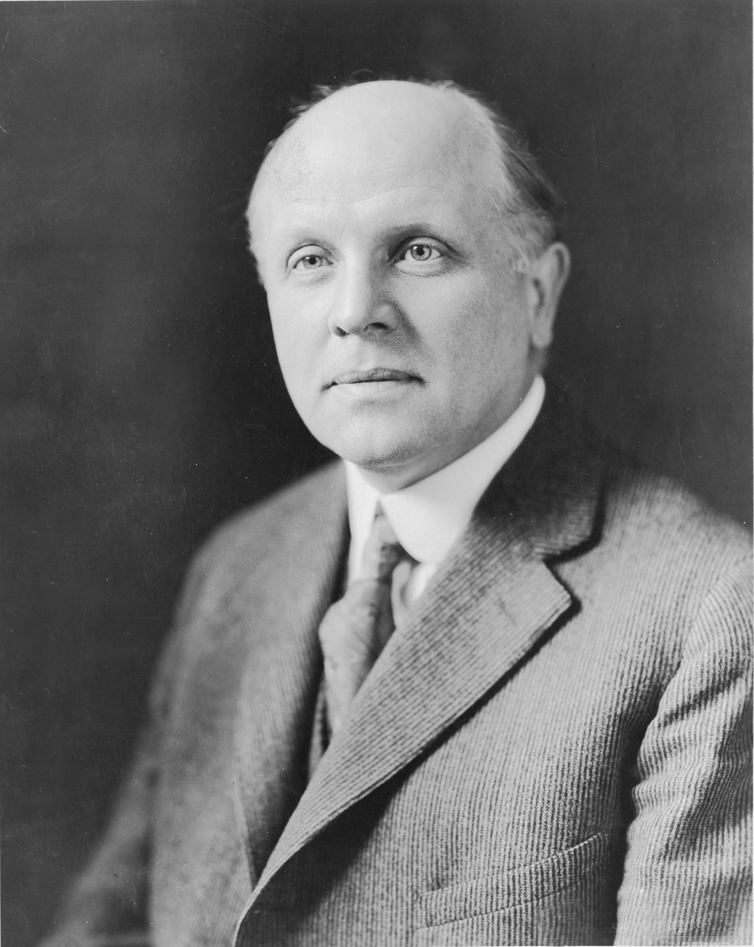
\includegraphics[width=0.6\textwidth]{Bingham.jpg}\\
				\large{\bf Eugene Cook Bingham}
			\end{center}
		\end{minipage}
	\end{center}
		\caption{レオロジーの創始者}
		\label{Bingham}
\end{figure}

日本では、それから約二十年後の 1951 年に第1回レオロジー討論会が開催されています。
学会としてレオロジー学会が設立されたのは、その二十年以上後の 1973 年になります。
ですから、学問と考えれば、それほど歴史が古いわけでもないことになります。
その後、現在に至るまでその発展は続いており、非常に多様な分野へと適応される範囲は広がってきています。

\subsection{レオロジーのやり方}

そもそも、物体の変形や流動に関する物理学は、古くから弾性論\index{だんせいろん@弾性論}や流体論\index{りゅうたいろん@流体論}として存在していました。
弾性論は Hooke の法則\index{ふっくのほうそく@Hooke の法則}を基本にして弾性固体を、そして、流体論はNewton の法則\index{ニュートンの法則@Newton の法則}により粘性を持つ単純な流体を対象として、物体の挙動を明確にしていたのでした
\footnote{
	Hooke の法則、Newton の法則については、後ほどきちんと説明しますので、安心してください。
}。
\begin{figure}[htb]
    \begin{center}
        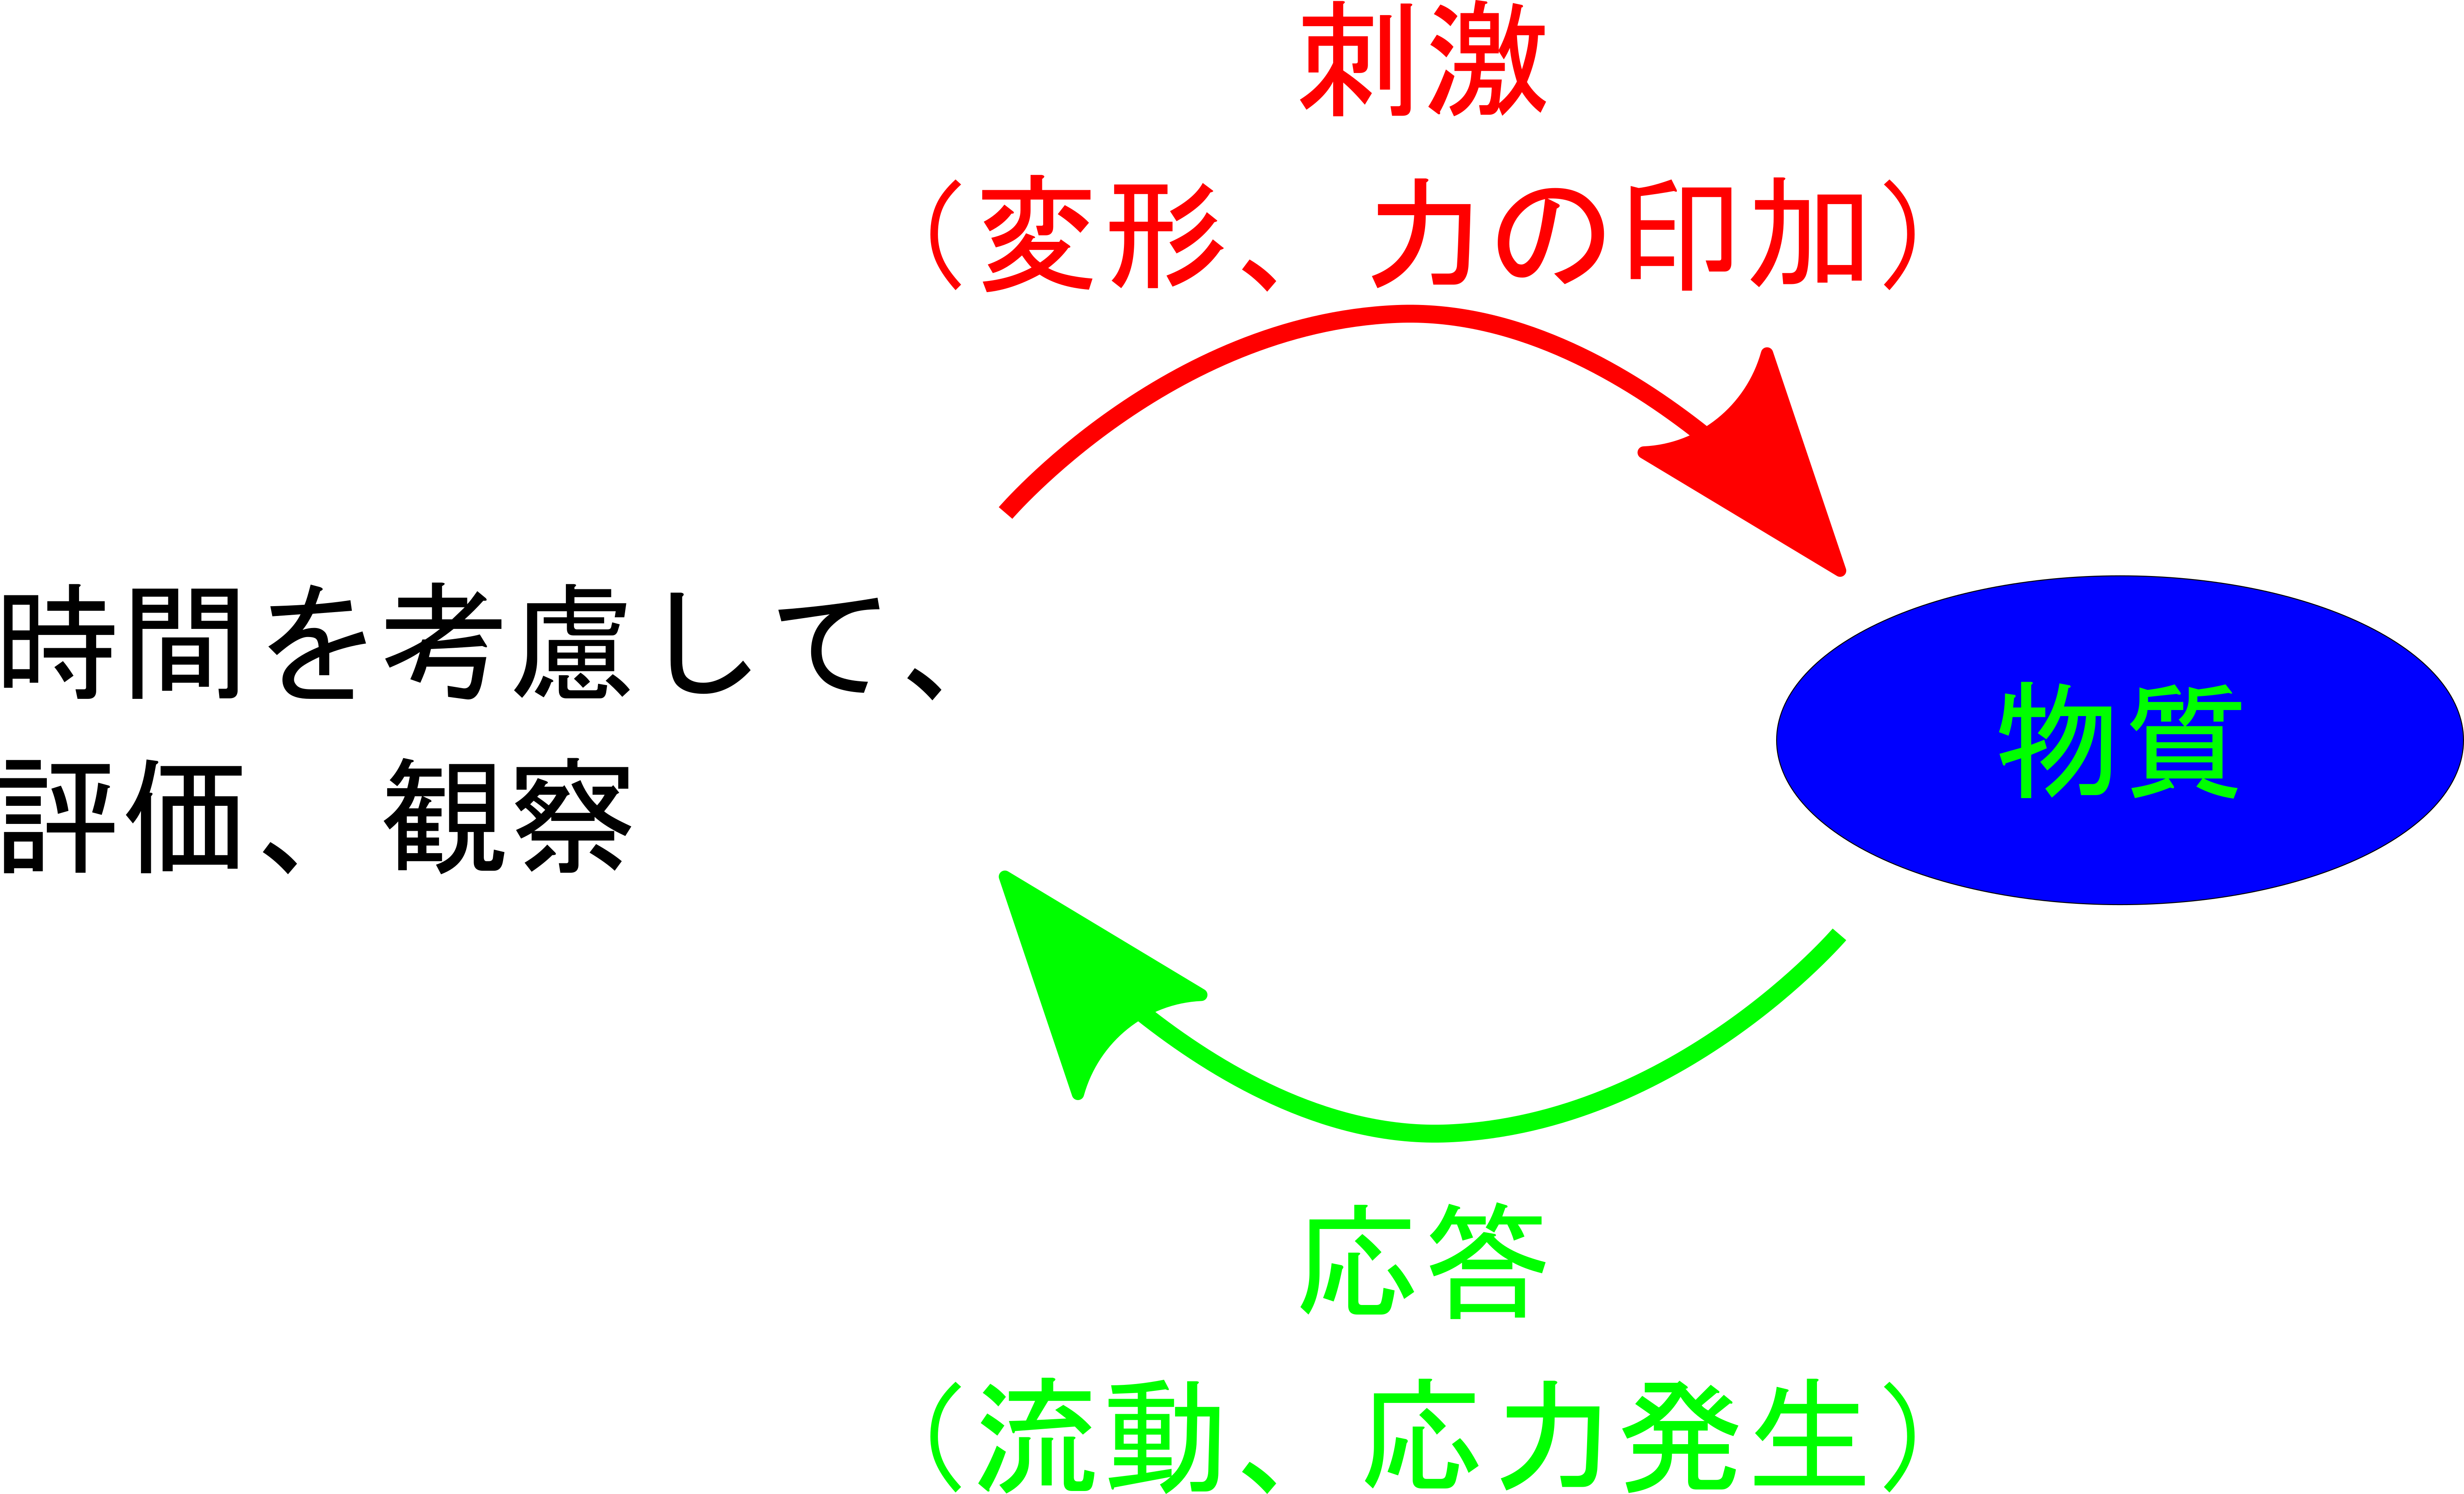
\includegraphics[width=.9\textwidth]{Rheo_method.png}
        \caption{レオロジーのやりかた}
        \label{yarikata}
    \end{center}
\end{figure}

レオロジーは、弾性固体とか粘性流体のような「理想的な物体」に限ること無く、我々が日々に遭遇する「一般にそこらに存在する物質や材料」を対象に含んでいます。
言い換えれば、対象を問わず、その変形と流動に関する事柄をすべて取り扱うということになり、物理学、化学、生物学、地学、医学、薬学、農学、食品学、家政学、時には心理学までをも含む多くの学問分野に横断的に関係する極めて学際的な学問となっています。

レオロジーは、そもそも科学の一分野として提唱されたわけですが、変形や流動というキーワードで物質や材料の特性を評価できることになりますから、実学として工学的にも大きな意味を持って来ています。
これが、広くレオロジーが用いられるようになった大きな要因となります。

レオロジーを測定する具体的な方法は、物質に外的な刺激を与えて、その応答としての変形や流動を測ることになります。
一般に、その刺激とは物質に力\index{ちから@力}や変形を与えることであり、応答としては時間という因子を意識しながら物質の流動や返してくる力\footnote{
	このあとに詳細を学びますが、このときの返してくる力は「応力\index{おうりょく@応力}」という物質内部での内力と呼ばれるものとなります。
}を測定することになります。
そして、このような測定を通して、物質の持つ各種の特性を比較することができるようになるわけです。

この考え方を簡単に書き直すと、図 \ref{yarikata} に示したようになります。

\section{会社の仕事とレオロジー}

ここでは、レオロジーの関わる分野が多様であることを確認し、その多様性を会社の仕事に生かしていくということについて考えてみましょう。

\subsection{レオロジーの関わる分野}

前述したように、1929年にアメリカにおいて、Bingham を中心としてレオロジー学会 The Society of Rheology (SOR) が設立されました。
日本では、それから約二十年後の 1951 年に第1回レオロジー討論会が開催されています。
その後、多様な分野へとその適応される範囲は広がってきています。

例えば、2019 年に開催された第 67 回レオロジー討論会に協賛した学会を見てみましょう。
\begin{screen}
	日本材料学会、プラスチック成形加工学会、高分子学会、日本化学会、日本物理学会、繊維学会、応用物理学会、化学工学会、
	強化プラスチック協会、日本ゴム協会、日本接着学会、日本セラミックス協会、日本木材学会、セルロース学会、日本機械学会、
	日本雪氷学会、日本混相流学会、日本流体力学会、可視化情報学会、日本食品科学工学会、日本家政学会、日本調理科学会、
	日本食品工学会、日本繊維機械学会
\end{screen}

非常に多様な学会が協賛しており、レオロジーという学問が学際的な特徴を有していることがわかります。

さらに、それぞれの学会が関連している分野を考えると、学術的な分類だけではなくて材料の種類や応用の範囲にしても、以下のように非常に幅広い分野に渡っていることが理解できます。
	\begin{itemize}
	\item
	  学術分野:化学、物理、生物、化学工学、応用物理、流体力学、地球物理学
	\item
	  高分子化学(科学):プラスチック、繊維、ゴム、強化プラスチック
	\item
	  材料:金属、セラミックス、木材
	\item
	  応用:機械、接着、塗料、食品化学、調理科学、家政学、成型加工
	\end{itemize}
	
したがって、レオロジーとは、高度に学際的な科学であると同時に、それぞれの要素技術が大きく異る多岐にわたる対象を、多様な切り口で議論していくことが出来るアプローチとも捉えられます。

\begin{figure}[htb]
	\begin{center}
		\includegraphics[width=.9\textwidth]{Katsuyou.png}
		\caption{レオロジーの活用}
		\label{katsuyou}
	\end{center}
\end{figure}

\subsection{会社の仕事とレオロジー}

次に、会社の仕事とレオロジーの関係について考えてみましょう。
この講座に参加されているみなさんの大多数は、会社に勤務されていると思います。
ここで、会社の社会的な意味について確認しておきましょう。

一般に、会社は営利団体であり、利益を生み出すことでその存在を継続させ、社会的な意義を果たしていくことになります。
そして、製造に関連する会社であれば、商品(製品)を作り出し、製造、販売することで、その利益を生じているわけです。

商品の開発の流れを簡単に言えば、原料から材料、そして商品へと価値を付与できるようにつなげていく過程と考えることができます。
そして、それぞれのステップで評価・解析に基づく、設計を行っていくわけです。
その設計の過程において商品に必要となる特性を評価する際に、レオロジーを活用することが多いわけです。
模式図とすれば、図 \ref{katsuyou} に示したようなイメージとなります。

\subsection{レオロジーと商品}

以前に図示(図 \ref{yarikata})したように、レオロジーとは物質に刺激を与えてその応答を評価観察することで、その特性を評価できるのでした。

では、商品化におけるレオロジー利用の、具体的な例を見てみましょう。
以下に示したように、人間の心地良さの定量化や、原料、材料の機能設計にレオロジーが活用されている事例が多くあります。
\large
	\begin{itembox}[l]{レオロジーが活用されている例}
		\begin{itemize}
			\item
			人間の心地良さの定量化にレオロジー的感覚で評価
			\begin{itemize}
				\item 食品工学における「舌触り」や「のど越し」のような食感の定量化。
				\item 肌触りの良い下着やノビの良い化粧品のような触感の定量化
			\end{itemize}
			\item
			原料、材料の機能設計にレオロジーを利用
			\begin{itemize}
			\item
				ショックのない運動靴やよく飛ばせるゴルフクラブのような力学特性の評価
			\item
				塗り易くて液だれしない塗料のような流動特性の評価
			\end{itemize}
		\end{itemize}
	\end{itembox}
\normalsize
したがって、少なくとも定性的に物事を評価するためには、レオロジーが非常に有効な方法であることが理解できるでしょう。

\section{人の感覚とレオロジー}
\label{sec:1_kankaku}

前節で、人間の心地良さのような感覚を評価するためにレオロジーが使えるという事例を示しました。
このことについて、もう少し詳しく考えてみましょう。

\subsection{人はみなレオロジスト}

\subsubsection{オノマトペとレオロジー}

オノマトペ\index{おのまとぺ@オノマトペ}とは、状態や感情を言葉に表したものであり、この語彙が多彩で豊富であることが日本語の大きな特徴の一つとなっています。
織物などの手触りのような質感を意味する言葉として、テクスチャという言葉もあります。
手触りだけでなく食品分野で食感を表現するためにも、テクスチャを表すオノマトペが多用されています。

レオロジーに、単純につながるような物性を表す言葉としては、「サラサラは低粘度、ドロドロは高粘度」や「ふにゃふにゃは低弾性、カチカチは高弾性」のようなものもありますし、これが、フワッフワとかモッチモチになると、一層感覚的な表現になってきます。
このような感覚は、別に若者言葉として特別なのではなくて、日本人には共通認識として通じる感覚になっています。
\begin{figure}[htb]
	\begin{center}
		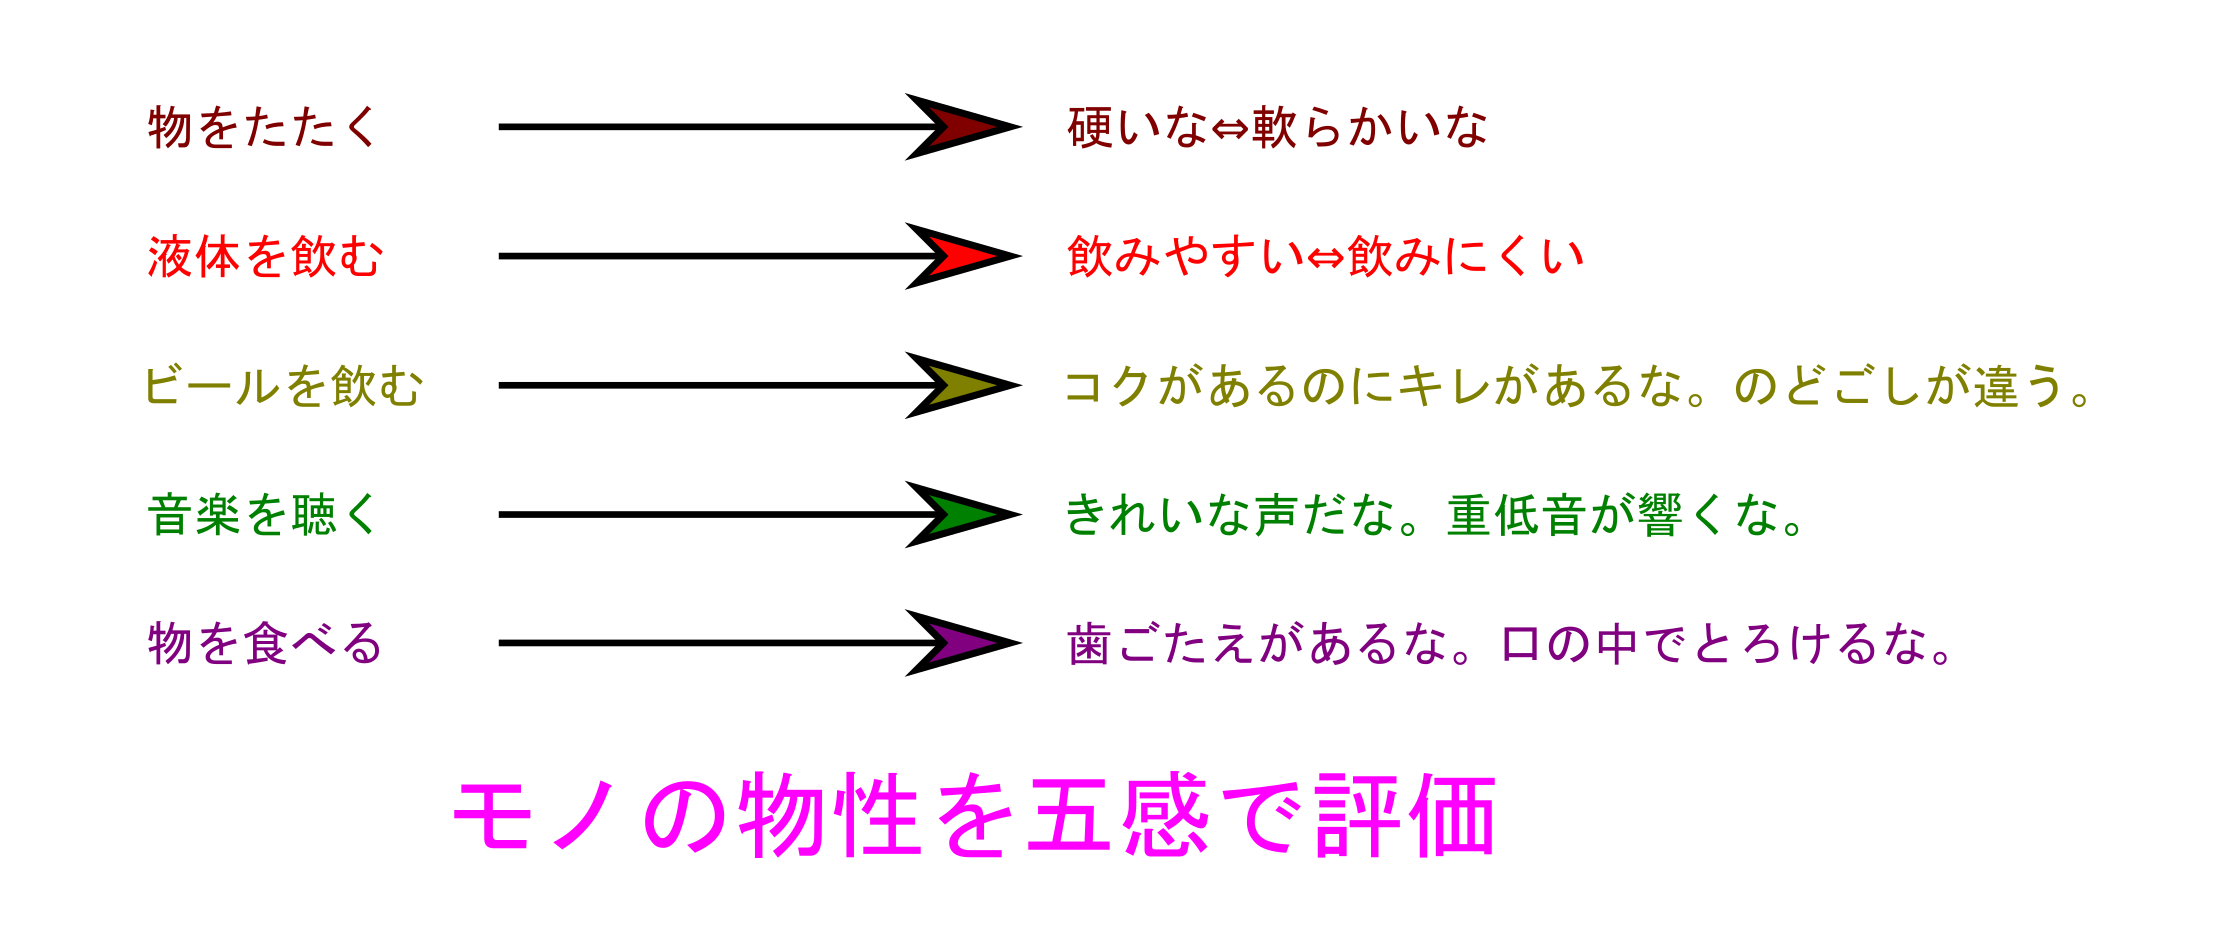
\includegraphics[width=.9\textwidth]{gokan.png}
		\caption{人間の五感とレオロジー}
		\label{gokan}
	\end{center}
\end{figure}

そして、このような言葉として物性やモノの有り様を表すことは、科学としてのレオロジーだけではなく、日常的に行われている評価なのです。

\subsubsection{人間の五感とレオロジー}

我々の生活の場において、なにかものを評価するときに、それを叩いてその音で判断することがあります。
具体的には、以下のような場面です。

\begin{itemize}
	\item 陶磁器の品質を見分ける
	\begin{itemize}
		\item 指先ではじいてその音を聞く
		\item 焼き上がり具合に応じて振動状態が変化し、陶器と磁器の見分けがつく。
	\end{itemize}
	\item スイカの熟し具合
	\begin{itemize}
		\item 熟れ過ぎたスイカは音が低くなる。
		\item 実の部分に微小な気泡が生じている。
	\end{itemize}
	\item 医者が打診によって診断
	\begin{itemize}
		\item お医者さんが指で胸やお腹を叩く。
		\item 音の響きで、内臓の腫れやうっ血を判断できる。
	\end{itemize}
\end{itemize}

こんな具合に、人は物質の状態を音で判断することができているわけです。

また、手触りでものの状態を判断することもやっています。
これらの行為は、ものを叩いたり触ったりして刺激を与えて、その応答を音で聞いたり手触りで感じたりしているわけですから、レオロジー評価を行っていると言うことにほかなりません。
すなわち、人間は五感を使ってレオロジーを行うレオロジストということになります。

\subsection{人間の判断基準は?}

しかしながら、オノマトペのような言葉としての表現はあくまでも感覚としての相対的な比較であり、感覚としての違いを何でどのように表すかが難しいわけです。

具体的な数値化のお話は後で行いますが、ここでは、人間の感覚の特徴について、もう少し考えてみましょう。

\subsubsection{ウェーバー比\index{うぇーばーひ@ウェーバー比}}

様々な刺激に対する人間の感覚的な評価について、ドイツの生理学者である E. Weber は、「人間の変化を感じ取る感覚量は、受ける刺激の差ではなく何倍になったかという比に依存する」という関係を見出しました。
\begin{align*}
	\text{ウェーバー比} = \dfrac{\Delta R}{R}= \dfrac{\text{増加量}}{\text{初期値}}
\end{align*}

\begin{figure}[htb]
	\begin{center}
		\begin{minipage}{0.45\textwidth}
			\large
			\begin{itembox}[l]{ウェーバー比}
				\begin{itemize}
					\item 人間の感覚量は、
					\item 受ける刺激の差ではなく、
					\item 何倍になったかという比
				\end{itemize}
			\end{itembox}
		\end{minipage}
		\begin{minipage}{0.45\textwidth}
			\large
			\begin{align*}
				\text{ウェーバー比} &= \dfrac{\Delta R}{R} \\
				&= \dfrac{\text{増加量}}{\text{初期値}}
			\end{align*}
		\end{minipage}
		\caption{ウェーバー比}
		\label{fig:weber}
	\end{center}
\end{figure}

この関係を数式で表すと、はじめに加えられる基準となる刺激量の強度を $R$ としたとき、人間が違いに気づくことができる閾値 $\Delta R$ との間に以下のような式が成立し、そのウェーバー比は事柄ごとに決まるということになります。

これを具体的に書くと、ある人が、10 の刺激が 20 になったときに「増加した」と気づくとしましょう。
このときの増加量は、10になりますから、ウェーバー比は 1 です。
その人は、20 の刺激が同じ増加量で 30 になってもその増加には気づかず、気づかせるためには 40 にする必要があるということになります。
言い換えると、「もともと強い刺激を基準とした場合、その違いを見分けることは難しい。$\Leftrightarrow$ 強い刺激には鈍感」ということになります。

当然、人の感覚は異なりますから、ウェーバー比の値は個々に異なりますが、大枠の傾向としてはこの様になっているわけです。

\subsubsection{フェヒナーの法則}

ヴェーバーの弟子である G. Fechner は、ヴェーバーの法則の式を微分方程式とみなして積分することにより、以下の対数法則を導き出しています。

すなわち、刺激量の強度 $R$ が変化する時、これに対応して人が感じる感覚量 $E$ は、以下のようになります。
\begin{align*}
	E = C \log R
\end{align*}
ここで $C$ は定数です。

この数式の示すことは、心理的な感覚量 $E$ は、刺激の強度の値 $R$ ではなく、その対数 $\log R $ に比例して知覚されるということになります。
具体的に言えば、100 の刺激が倍に増加して 200 になるときの感覚量と、200 の刺激が倍に増加して 400 になるときの感覚量の変化は等しいわけです。

\subsubsection{ウェーバー・フェヒナーの法則\index{うぇーばー・ふぇひなーのほうそく@ウェーバー・フェヒナーの法則}}

二人の師弟によって示された上記の関係を合わせてまとめると、
\large
	\begin{itembox}[l]{ウェーバー・フェヒナーの法則}
		\begin{itemize}
			\item 刺激量の差だけではわかりにくい
			\begin{itemize}
				\item 相対変化は見やすいが、絶対的な差はわかりにくい。
			\end{itemize}
			\item 基準値によって閾値が変わる
			\begin{itemize}
				\item 元々強い刺激の変化には鈍感
				\item 基準値をそろえたほうがわかりやすい。
			\end{itemize}
			\item 差ではなく比で比較する
			\begin{itemize}
				\item 桁数の違いで感じるということが大事。
			\end{itemize}
		\end{itemize}
	\end{itembox}
\normalsize
というようなことになります
\footnote{
	ここで議論したような人間の感覚に関わるような分野は、心理レオロジー(サイコレオロジー)と呼ばれており、定性的な感覚量を定量化するためには重要な考え方になっています。
}
。

このように考えると、レオロジー評価を料理に例えられる場合の以下のような表現も理解できてきます。
\begin{itemize}
	\item レオロジーで何がわかるのか?
	\begin{itemize}
		\item 隠し味の調味料がわかるわけではない!
		\item 調味料を加えた時に、味がどう変化したのかがわかる。
	\end{itemize}
	\item 比較試料を用いて、相対値評価をする
	\begin{itemize}
		\item 絶対値評価はできない。
		\item 対数的な応答と考えれば、理解しやすい。
	\end{itemize}
\end{itemize}

\section{レオロジーを理解するために}
\subsection{レオロジーの難しい点}

前述のように、レオロジーという考え方自体は非常に単純で分かりやすいものなんですが、
実際に比較しようとするととたんに面倒くさくなってくるものでもあります。

\subsubsection{似たものを比べると?}

例えば、身近にある水と蜂蜜を比べてみましょう。
\begin{itemize}
	\item 水
	\begin{itemize}
		\item 箸で簡単にかき混ぜることができる。
		\item たやすくコップに注ぎ込むことができる。
	\end{itemize}
	\item 蜂蜜
	\begin{itemize}
		\item 容易にかき回すことができない。
		\item 入れ物を傾けても、流れにくい。
	\end{itemize}
\end{itemize}

触ってみたときの手応えとして比べるのであれば、これらの二つがずいぶん違うことは簡単にわかります。
しかしながら、その違いはあくまでも感覚としての相対的な比較であり、この違いを何で表すかが難しいわけです。

粘っこい者同士となると一層困難になります。
例えば、ハチミツとマヨネーズとを比べることを考えてみましょう。 
これらを比較するためには、何らかの客観的な判断基準が必要となってくることになります。

\subsubsection{言葉の使い方が曖昧}

もう一つの面倒くさいこととして、レオロジーでは多様な言葉が用いられる場合が多いことが挙げられます。
これは、\ref{sec:1_kankaku} 節 (\pageref{sec:1_kankaku} ページ) で後述するように、
レオロジーが人間の直感的な評価を行いやすいためだと考えることができます。
その結果として、抽象的な言葉や指示代名詞による、あまりにもイメージに偏った議論に陥りがちになるのです
\footnote{まあ、流石に以下のようなことを本当に言う人は少ないのですが、それに近いことを口走っていることはよく見かけます。
	
「この時はこう、あの時はああ。」$\Leftarrow$ それなら。今はどの時?}。

例えば、以下に示したように、言葉の定義や使い方が不明確だとわかりにくくなります。
% \begin{shadebox}
	
	\begin{itemize}
		\item わかり易そうで、油断するとよくわからない表現(逃げ言葉?)\\
		たとえば、以下に示したような言葉は、レオロジーの説明によく出てきていますが、
		具体的に理解しようとするとその意味がとたんにわからなくなりませんか?
		\begin{itemize}
			\item 「応力集中が粘弾性により緩和します。」
			\item 「チクソ性の高い液体は液だれしにくい。」
			\item 「非Newton 流体の特徴的な流動を設計しなければいけない。」
		\end{itemize}
		\item 数式の羅列で数学的なお話\\
		確かに、数式を使いこなせれば言葉の定義の不明確さは解消できるのですが、数式が突然天下りで出てきても、
		内容がイメージできるわけでもありません。なお、以下の表式は見た目がややこしそうというだけの例です。
		\begin{itemize}
			\item 例えば、一般化マックスウェルモデルの動的貯蔵弾性率を表す数式\\
		\end{itemize}
	\end{itemize}
	\vspace{-7mm}
	\begin{align*}
		\displaystyle G'(\omega) = \int_{-\infty}^{\infty} \mathcal{H}(\ln \tau)\dfrac{\omega^2 \tau^2}{1 + \omega^2 \tau^2} \mathrm{d}(\ln \tau)
	\end{align*}
% \end{shadebox}

さらに、レオロジーの対象は非常に幅広いものであることも、混乱しやすいもう一つの原因となります。
以下に例を示したように、食感や手触りから、材料の機能性の設計に至るまで、非常に幅広い分野でレオロジーの言葉は使われています。
これらの言葉も、使っている人に応じて微妙に言葉に込めた意味合いが異なっていますので、混乱しやすいものとなります。
% \begin{shadebox}
	\begin{itemize}
		\item 人間の心地よさをレオロジー的感覚で評価
		\begin{itemize}
			\item 「タピオカ」の喉越しのツルンとした感覚
			\item 肌触りのよい下着
		\end{itemize}
		\item 機能設計にレオロジーを利用
		\begin{itemize}
			\item ショックのない運動靴
			\item 塗り易くて液だれしない塗料
		\end{itemize}
	\end{itemize}
% \end{shadebox}

\subsubsection{よくある状態}

我々の身の回りで、レオロジー関連で実際によくある状態として、以下のようなものがあります。
たとえば、「頭で考えずに手を動かして、とにかく測れ」と言われたり、「まずよく調べてから測定しよう」と言われたりして、
どうすればいいのか判らなくなったりします。
そこで、自身が素人であることを自覚して周りのマネをしようとしても、近くに先輩がいなかったり、
そもそも新しい問題については誰も先輩になれなかったりもするわけです。
\large
	\begin{itembox}[l]{よくある状態}
		\begin{itemize}
			\item ありがちな両極端
			\begin{itemize}
				\item 脳みそ筋肉状態
				\begin{itemize}
					\item とにかく測れ
				\end{itemize}
				\item 頭でっかち
				\begin{itemize}
					\item 理屈ばかりで手が動かない
				\end{itemize}
			\end{itemize}
			\item 誰もが、最初は素人 $\Leftrightarrow$ うまくやっている人の物まねが手っ取り早い
			\begin{itemize}
				\item でも、近くにいい先輩がいないときは?
				\item 新しい問題へのアプローチは?
			\end{itemize}
		\end{itemize}
	\end{itembox}
\normalsize

\subsection{理解へのアプローチ}
こんなときに、おすすめしたいのが、
\begin{center}
	\Huge{\bf「急がば回れ」}
\end{center}
という、キーワードになります。

すなわち、慌てて結果を出そうとするのではなく、心を落ち着けてやるべきことを明確化してイメージすることから始めてみることをお勧めします。

レオロジーというややこしいものでも、イメージとして全体像をザックリと捕まえることができれば、理解は一気に容易になります。

\subsubsection{見える化のすすめ}

イメージとして捉えるためには、自分の捉えるべき問題を自分の中に落とし込むことが大事です。
そのためには、モチベーションを高くすることが重要だと思います。
\large
\begin{itembox}[l]{お勧めの考え方}
	\begin{itemize}
		\item 「何のためにやりたいのか?」を明確に。
		\begin{itemize}
			\item 目的がわからないと、ゴールが見えない。
			\item 仕事であれば、上司とよく相談。
			\item 自己啓発であれば、自分の本心をよく見極める。
		\end{itemize}
		\item 「何をやりたいのか?」を常に意識しながら、
		\begin{itemize}
			\item 因果関係をはっきりと
			\begin{itemize}
				\item 因 $\Leftarrow$ 原因
				\item 果 $\Leftarrow$ 結果
			\end{itemize}
			\item 図として捉える
			\begin{itemize}
				\item 複雑な実事象をできるだけ単純化
				\item 一目で理解できるように  
			\end{itemize}
		\end{itemize}
	\end{itemize}
\end{itembox}
\normalsize



つまり、たとえ会社の仕事として命令されたような事項であっても、「何のためにやりたいのか」という目的と
「何をやりたいのか」という目標をきちんと設定することが最も大事になるのです。
他人事ではなく自分の問題として捉えることで、やる気が全く変わってくるものです。

そして、因果関係をはっきりとさせながら、その関係を図として単純化したイメージが持てるようになれば、
目標とそこに到達するための手段もクリアーに落とし込むことが出来ると感じています。

\subsubsection{色々なモデル化\index{もでるか@モデル化}}
それでは、レオロジーという道具を理解して、私達は何をやりたいのでしょうか?

この答えは、みなさんがそれぞれ異なっているでしょう。

参考までに著者の場合を書けば、私は「様々な条件のもとで幅広い検討対象に対してでも当てはめることの出来るような、
汎用的なモデル」が欲しいと考えています。
このモデルは、多様な実験事実を「尤もらしく」説明できるものであってほしいと考えています。
このような考え方ができるようになることで、表面的には異なる問題に見えるようなものの本質を捕まえることが出来、
普遍的な問題として捕まえることが出来ると信じています。
特に、レオロジーのようにとらえどころのないややこしい問題に対しては、適度に単純化したモデルが有効だと感じてきました。

これからの具体的な説明の中において、この「モデル化」という考え方についても、実際の例を上げて説明していきます。

\large
\begin{itembox}[l]{モデル化のすすめ}
	\begin{itemize}
		\item 適度な深さで尤もらしく
			\begin{itemize}
				\item 簡単すぎるものは例外が多い。
				\item 複雑化しすぎても過適応
				\begin{itemize}
					\item n個のデータを、n次の関数でフィット
					\item 個々の現象にだけ適応可能
					\item モデル化する意味がない
				\end{itemize}
			\end{itemize}
		\item 欲しいもの
		  \begin{itemize}
			\item 汎用的に使えるモデル
			\item 尤もらしく、実験事実を説明できるもの
		  \end{itemize}
		\end{itemize}
\end{itembox}
\normalsize

\section{この章のまとめ}
この章では、レオロジーという「考え方」についての説明を行い、会社の仕事にどのように役立つかを考え、
「おすすめの理解へのアプローチ」について紹介しました。
\begin{boxnote}
	\large
	\begin{itemize}
		\item 「レオロジー」という言葉の歴史的背景を振り返り、その流れを確認
		\item レオロジーが関わる分野が広範囲に渡り、会社での商品開発に有用
		\item 人間の直感とレオロジーの親和性が高いこと
		\item 「おすすめの理解へのアプローチ」について紹介
	\end{itemize}
\end{boxnote}

\newpage

\begin{longartdeco}
	\begin{center}
	\emph{コラム:緩和とリラックス}	
	\end{center}

	レオロジーという学問は、その成り立ちをベースにすれば、「流れるものの流れ方を考える学問」と捉えることができます。
	
	単純な応答を示す水のように、明らかに液体的な性質が主となってい場合には、あまり面倒なことを考える必要はありません。
	この場合は、変形速度と応力の関係を表す比例定数である粘度を決定すれば、流れ方の特徴を理解したことになります。
	このような流体は、初期の研究を行った Newton に因んで Newton 流体と分類されています。
	
	でも、世の中の大多数の物質はそれほど単純ではありません。
	一般に、固体的な性質と液体的な性質を兼ね備えた「粘弾性」という性質を持っている物質が多数派となっています。
	
	レオロジーでは、流れるということを「変形という刺激を与えた結果として生じる応答」と考えます。
	このような考え方に立てば、与えた刺激(変形)が消滅していく過程こそが「刺激が緩和していく」ということに対応します。
	したがって、粘弾性を示す物質においては、その「緩和現象」が重要になってくることになります。
	
	最後にゆったりとしたお話で締めましょう。
	緩和という言葉は、英語ではリラックスとなります。
	この語源はラテン語で、「緩んた状態(laxare)へ戻す(re)」ということを意味しているようです。
	昼間の仕事時間に、職場で拘束されて固体的にきちんと振る舞っていたサラリーマンが、
	自宅に帰ってソファーの上でだらけて液体的にリラックスしていく過程も緩和なんでしょうね。

\end{longartdeco}

\newpage

\question{演習問題 1}
内容を振り返るために、以下に示した文章例の中から適切な記述のものを複数選んでください。
\begin{qlist}
	\qitem レオロジーとはどのようなものでしょうか?
		\begin{qlist2}
			\qitem レオロジーとは「物質の変形と流動に関する科学」であり、これまでの物理理論とはかけ離れた新規な測定技術です。
			\qitem レオロジーのベースとなる物体の変形や流動に関する物理学は、古くから弾性論や流体論として存在していました。
			\qitem 弾性論はフックの法則を基本にして弾性固体の力学的な性質を記述し、流体論はニュートンの法則により粘性を持つ流体の流れ方の挙動を明確にします。
			\qitem レオロジー測定は、物質の変形や流動を測って、そこに加えられた刺激を推定する逆問題を解きます。
			\qitem レオロジー測定を通して、物質の持つ各種の特性を比較することができるようになります。
    \end{qlist2}
    \vspace{3mm}
	\qitem 会社の仕事とレオロジーとの関係について確認してみましょう。
		\begin{qlist2}
			\qitem レオロジーという学問は高度に学際的な科学であり、同時に、それぞれの要素技術が大きく異る多岐にわたる対象を多様な切り口で議論していきます。
			\qitem レオロジーは、物質の特性を絶対値として測定する方法で、物質に含有される成分を定量的に分析することができます。
			\qitem 商品の開発の「原料から材料そして商品へと仕立てる過程」において、特性の評価にレオロジーを活用することができます。
            \qitem 例えば、人間の心地良さの定量化や、原料、材料の機能設計にレオロジーが活用されている事例が多くあります。
            \qitem 人間の感覚のような抽象的なものは定量化する方法がありませんから、できるだけ過去の記憶や勘を働かせることで設計を進めるしかありません。
    \end{qlist2}
    \vspace{3mm}
	\qitem 人がもっている感覚とレオロジーとはどのような関係があるのでしょうか?
		\begin{qlist2}
            \qitem オノマトペとは様々な状態や感情を言葉に表したものであり、レオロジー的な違いを定性的に表現できます。
            \qitem 人間は身の回りにある様々な状態や感情に言葉を与えますが、そのような定性的な評価はレオロジーとは関係ありません。
			\qitem 人間は、ものを叩いたり触ったりして刺激を与えて、その応答を音で聞いたり手触りで感じることで、レオロジー評価を行う事ができます。
			\qitem 人間のレオロジー的な感覚を表現したウェーバー・フェヒナーの法則があり、基準とする値に応じて違いを見極める閾値が変わります。
            \qitem 人間の感覚は強い刺激の変化にとても敏感で、絶対的な差を感じることができます。
    \end{qlist2}
    \vspace{3mm}
	\qitem レオロジーを理解するために考えるべきことは?
		\begin{qlist2}
			\qitem 人間は手触りでレオロジー的な違いを判断できますが、定量的な評価を判断することはあまりうまくできません。
            \qitem 感覚的な違いを言葉で表せば、十分に人に伝わる定量的な評価になります。
            \qitem 以前に実施した実験の結果は実験事実なのだから、その内容の整合性など考えることなく過去の知見として使っていけます。
			\qitem 著者のおすすめは、標語的には「急がば回れ」であり、慌てずに、イメージとして全体像をザックリと捕まえることができれば、理解は一気に容易になると期待しています。
			\qitem 会社の仕事として命令されたような事項であっても、「何のためにやりたいのか」という目的と「何をやりたいのか」という目標をきちんと設定することが最も大事になります。
		\end{qlist2}
\end{qlist}

\question{演習問題 2}
内容を振り返るために、テキストで用いた言葉を使って簡単な穴埋めを行ってください。

\begin{qparts}
    \qpart 「レオロジーとは」について、以下の\qbox{(a)}から\qbox{(i)}までのカッコを埋めてください。
    \begin{qlist}
      \qitem レオロジーとは「物質の\qbox{}に関する科学」であり、既存の弾性論や流体論をベースとして、物質の持つ各種の特性を比較することができる学問です。
      決して新規な\qbox{}ではなく、過去の\qbox{}を利用していく必要があります。
      \qitem レオロジーの対象は多岐にわたりますが、基本的に物質の特性を\qbox{}する技術であり、\qbox{}が主となります。
      \qitem 人間のレオロジー的な能力はとても高く、様々な違いを定性的に感じることができます。ただし、その\qbox{}に感じるだけであり、また、基準に応じて\qbox{}することを理解する必要があります。
      \qitem レオロジーが相対的な比較であることをきちんと理解して、落ち着いて\qbox{}で議論しましょう。また、\qbox{}を明確にすることはとても大事です。
    \end{qlist}

    \begin{itembox}[l]{選択肢}
      \begin{center}
        \begin{tabular}{lllll}
                1. 目的と目標&2. 差を相対的に&3. 相対的に比較&4. 定性的な評価 & 5. 閾値が変化 \\
                6. 変形と流動&7. 多様な知見&8. わかり易い言葉 & 9. 測定技術
        \end{tabular}
      \end{center}
    \end{itembox}
\end{qparts}

\question{演習問題 3}
\begin{qparts}
    \qpart 「何をなんのためにやりたいのか」という目的や目標は皆さんそれぞれのものをお持ちであり、そのためにレオロジーを学ばれているのだと思います。
    折角の機会ですから、一度ご自身の有りたい姿について考えをまとめてみてはいかがでしょうか。

    以下に、かんたんに設問の形で項目を上げてみました。
    \vspace{-2mm}
    \begin{qlist}
        \qitem ご自分の仕事を、全く事前の知識を持たない他の人にでも理解できるように説明してみましょう。
        \qitem その仕事の中での、ご自分の役割をシンプルに表現してみてください。
        \qitem ご自分の役割の中で、何をやらなくてはいけないと感じていますか?
        \qitem その使命は、何のためにやっているのでしょうか?
        \qitem 上述の状態の中で、レオロジーにはどのようなことを期待していますか?
    \end{qlist}
    \vspace{-2mm}
    \qpart もしもご相談されたいことがあれば、書いていただければ相談に乗ります。(なお、こちらは提出は義務ではありません。)
\end{qparts}
\end{document}

\chapter{レオロジーを始める前に}
\documentclass[uplatex,dvipdfmx,a4paper,11pt]{jsreport}

\usepackage{docmute}


% 数式
\usepackage{amsmath,amsthm,amssymb}
\usepackage{bm}
% 画像
\usepackage{graphicx}

\usepackage{multirow}
\usepackage{wrapfig}
\usepackage{ascmac}
\usepackage{xcolor}


\usepackage{makeidx}
\makeindex

\graphicspath{{../../_Figures//}{../../_Figures/Rheology/}}

\usepackage{qrcode}
\setlength\lineskiplimit{0pt}
\setlength\normallineskiplimit{0pt}

\usepackage{qexam}

\usepackage{titlesec}
\titleformat*{\section}{\Large\bfseries}
\titleformat*{\subsection}{\large\bfseries}
\titleformat*{\subsubsection}{\normalsize\bfseries}
\titleformat*{\paragraph}{\normalsize\bfseries}

% ページ設定
% \pagestyle{empty}
% 高さの設定
\setlength{\textheight}{\paperheight}   % ひとまず紙面を本文領域に
\setlength{\topmargin}{-5.4truemm}      % 上の余白を20mm(=1inch-5.4mm)に
\addtolength{\topmargin}{-\headheight}  % 
\addtolength{\topmargin}{-\headsep}     % ヘッダの分だけ本文領域を移動させる
\addtolength{\textheight}{-40truemm}    % 下の余白も20mmに%% 幅の設定
\setlength{\textwidth}{\paperwidth}     % ひとまず紙面を本文領域に
\setlength{\oddsidemargin}{-5.4truemm}  % 左の余白を20mm(=1inch-5.4mm)に
\setlength{\evensidemargin}{-5.4truemm} % 
\addtolength{\textwidth}{-40truemm}     % 右の余白も20mmに
% 図と本文との間
%\abovecaptionskip=-5pt
%\belowcaptionskip=-5pt
%
% 全体の行間調整
% \renewcommand{\baselinestretch}{1.0} 
% 図と表
%\renewcommand{\figurename}{Fig.}
%\renewcommand{\tablename}{Tab.}
%

% \makeatletter 
% \def\section{\@startsection {section}{1}{\z@}{1.5 ex plus 2ex minus -.2ex}{0.5 ex plus .2ex}{\large\bf}}
% \def\subsection{\@startsection{subsection}{2}{\z@}{0.2\Cvs \@plus.5\Cdp \@minus.2\Cdp}{0.1\Cvs \@plus.3\Cdp}{\reset@font\normalsize\bfseries}}
% \makeatother 

\usepackage[dvipdfmx,%
 bookmarks=true,%
 bookmarksnumbered=true,%
 colorlinks=false,%
 setpagesize=false,%
 pdftitle={数式に頼らない直感的理解による材料設計のためのレオロジー⼊⾨},%
 pdfauthor={佐々木裕},%
 pdfsubject={},%
 pdfkeywords={レオロジー; 材料設計; }]{hyperref}
\usepackage{pxjahyper}

\usepackage{plext}

\usepackage{niceframe} 
\usepackage{framed}
\newenvironment{longartdeco}{%
  \def\FrameCommand{\fboxsep=\FrameSep \artdecoframe}%
  \MakeFramed {\FrameRestore}}%
 {\endMakeFramed}
 
\usepackage{siunitx}

\newcommand{\rmd}{\mathrm{d}}

\begin{document}

\setcounter{chapter}{1}
\chapter{レオロジーを始める前に}

\section*{この章の内容}

この章では、「レオロジーをはじめる前に」として、レオロジーを理解するために必要となる準備を行っていきます。
具体的には、数学及び物理の基本となるような考え方についての確認から手を付けていきます。

以下に、この章で議論する内容について簡単にまとめました。

	\begin{boxnote}
		\large
		\begin{itemize}
			\item 数学的な事項の確認
			\begin{itemize}
				\item 数学的に書き表すときに基本となる「関数」について
				\item 事象を単純化して考えるときに重要な「線型性」
			\end{itemize}
			\item 物理的に考えるときに必要になること
			\begin{itemize}
				\item 物理モデルと線型性
				\item 物理モデルを理解するために、「量」、「次元」、「単位」
			\end{itemize}
		\end{itemize}
	\end{boxnote}

\section{数学的な事項の確認から}

具体的なレオロジーの議論に入る前に、これからの議論に必要となる数学の基礎的な事項について確認していきましょう。
ここでは、それほど難しいものを考えているわけではありません。
レオロジーを理解するために、どうしても必要となる中学から高校レベルの基本的なことを思い出していただくことになります。

具体的には、「関数と線型性」ということについて少しずつイメージを明確にしていくようにしましょう。

\subsection{関数\index{かんすう@関数}について}
\subsubsection{直感的理解}
まず、関数を直感的に理解することから始めます。
\begin{figure}[htb]
	\begin{center}
		\begin{minipage}{0.5\textwidth}
			\large
			\begin{itembox}[l]{関数とは?}
				\begin{itemize}
					\item ある変数 $x$ に依存して決まる出力 $y$ を決める方法(右上)
					\item 入力 $x$ に対して出力 $y$ を与える変換装置(ブラックボックス)のようなもの(右下)
				\end{itemize}
			\end{itembox}
			
		\end{minipage}
		\begin{minipage}{0.4\textwidth}
			\begin{center}
			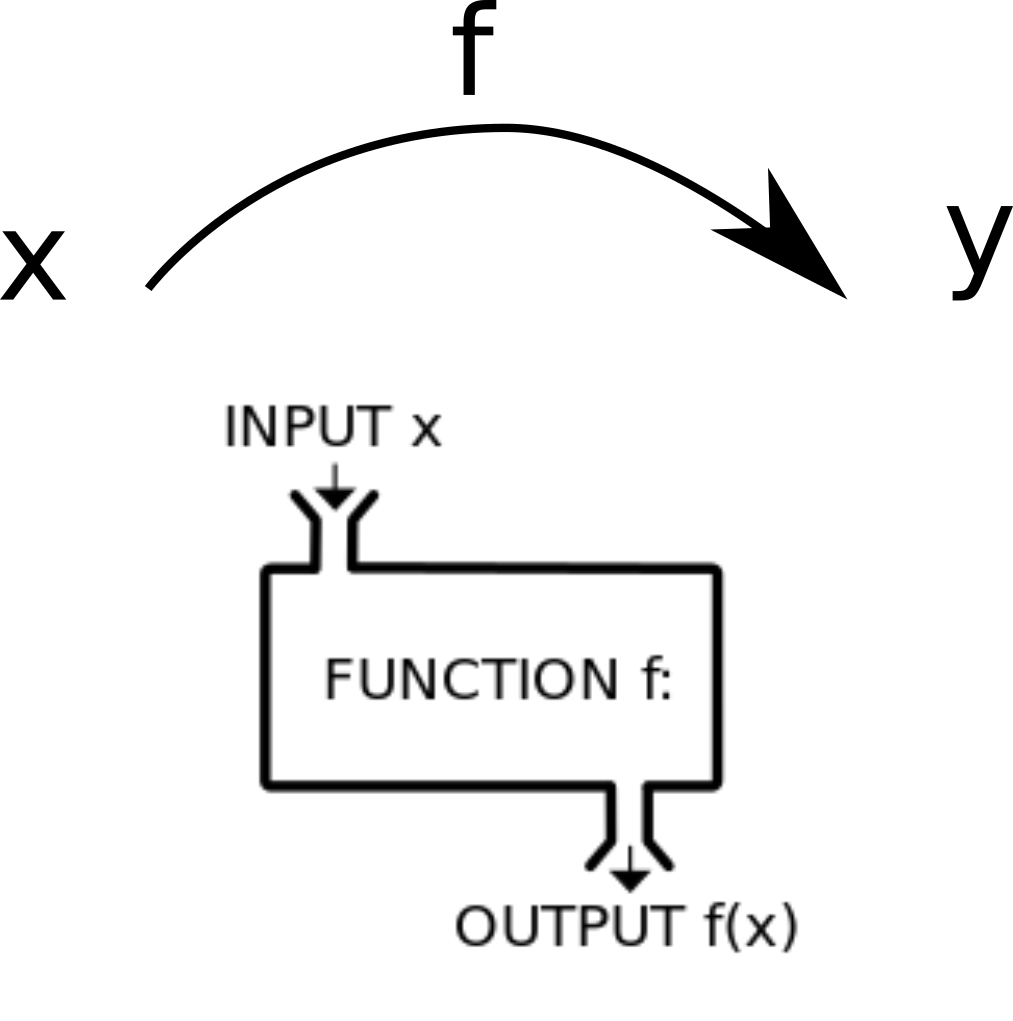
\includegraphics[width=.9\textwidth]{function.png}
			\end{center}
		\end{minipage}
		\caption{関数とは}
		\label{function}
	\end{center}
\end{figure}

関数とは、2つの変数 $x$ と $y$ があり、入力を $x$ で表したときに、その出力 $y$ を決定する規則というようなイメージと捉えることができます。
一般に、関数は、英語の function の頭文字を使って $f$ で表され、どの変数を入力として用いている関数であるかをカッコの中に変数を書くことにより示します。
\begin{align*}
	y&=f(x) \\
	\text{出力}&=\text{関数} \left(\text{入力} \right)
\end{align*}

関数の役割を考えてみると、入力を変換装置に入れた結果として出力が現れるわけですから、入力と出力との間の関係を表していると考えることもできます。

\subsubsection{関数と写像}
また、関数\index{かんすう@関数}というのは、数の集合に値を取る写像の一種と考えることもできます。

定義域と呼ばれる左の集合から、値域となる右の集合への射影を行う方法が、関数ということになります。
\begin{figure}[htb]
	\begin{center}
		\begin{minipage}{0.45\textwidth}
			\large
			\begin{itembox}[l]{集合と関数}
				\begin{itemize}
					\item 左の集合(定義域)から
					\item 右の集合(値域)へ
					\item 射影する方法が関数
				\end{itemize}
			\end{itembox}
		\end{minipage}
		\begin{minipage}{0.45\textwidth}
			\begin{center}
			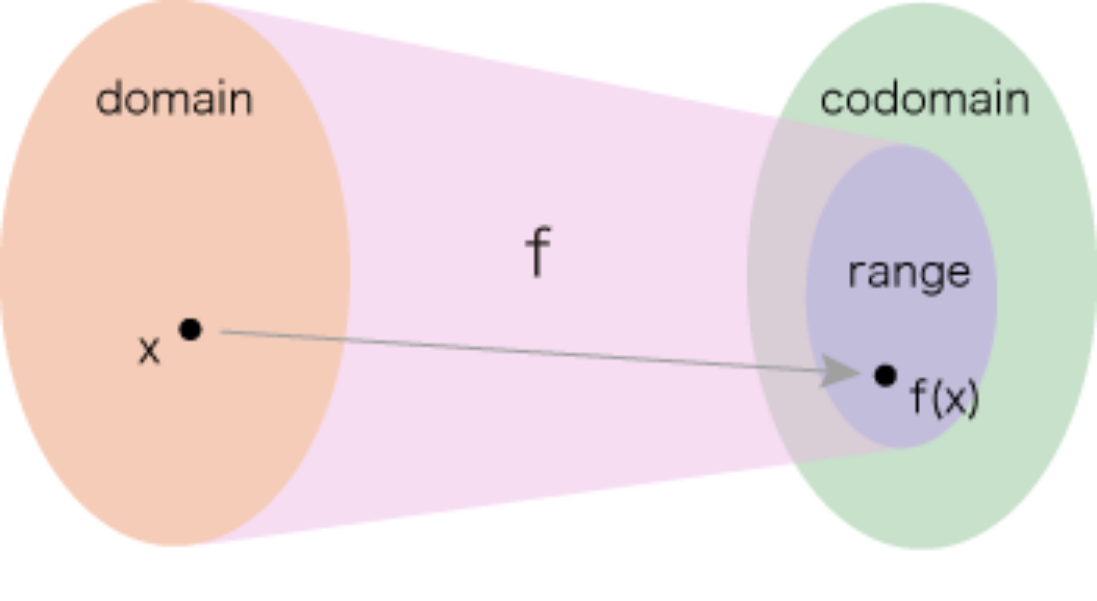
\includegraphics[width=.9\textwidth]{function_2.png}
			\end{center}
		\end{minipage}
		\caption{関数と写像}
		\label{function_2}
	\end{center}
\end{figure}

\subsubsection{グラフとは}
グラフ\index{ぐらふ@グラフ}とは、入力と出力との関係を平面図
\footnote{
	本当は、二次元とは限らずに多次元空間で表したグラフも使われていますが、直感的な理解は平面図にまさるものはありません。
}に示したものであり、視覚的にその関係を理解しやすくしたものと考えることができます。

具体的には、入力 $x$ に対応して決まる出力の点を平面上にたくさん書き込んで、それを連続的に(直線または曲線で)つないだものがグラフとなります。
\begin{figure}[htb]
	\begin{center}
		\begin{minipage}{0.45\textwidth}
			\large
			\begin{itembox}[l]{関数を表すグラフ}
				\begin{itemize}
					\item 横軸が入力
					\item 縦軸が出力
					\item 関数の値を連続的に
				\end{itemize}
			\end{itembox}
		\end{minipage}
		\begin{minipage}{0.45\textwidth}
			\begin{center}
			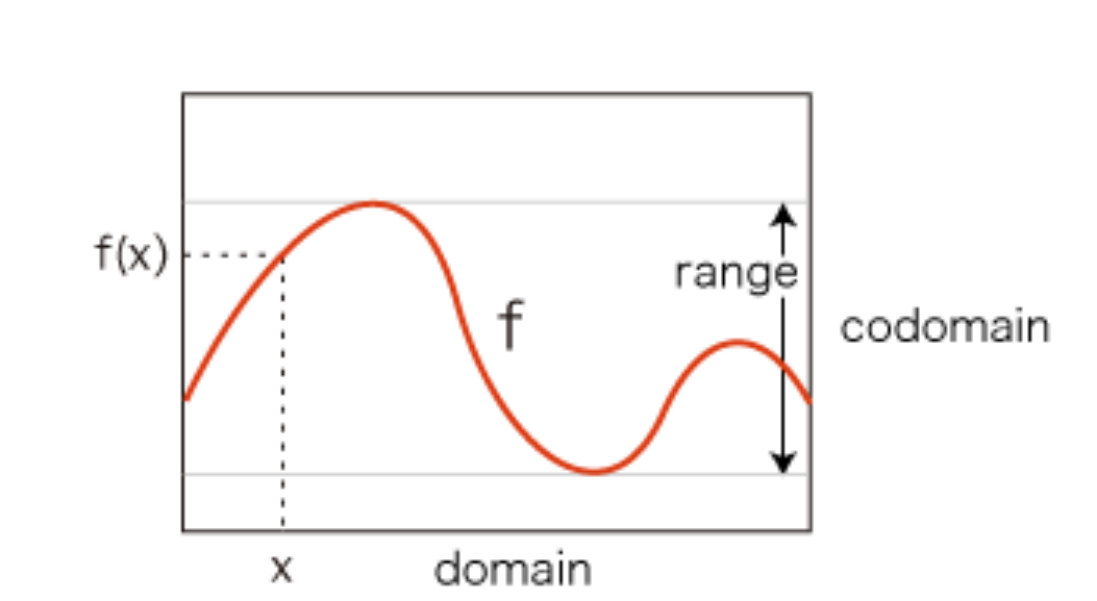
\includegraphics[width=\textwidth]{function_3.png}
			\end{center}
		\end{minipage}
		\caption{関数とグラフ}
		\label{function_3}
	\end{center}
\end{figure}


図 \ref{function_2} の右に示した集合間の写像を二次元のグラフに表すと、図 \ref{function_3} のように値を決める赤い曲線が関数を表すというイメージとなります。
このグラフに表した関数の形を見ることで、入力と出力との関係を直感的に理解することができます。

\subsection{線型\index{せんけい@線型}という意味を理解しよう}

\subsubsection{線型とは?}
線型\index{せんけい@線型}という言葉を直感的にイメージすると、グラフに表した時に原点を通る直線となるような性質と捉えることができます。

数学的にもう少しだけきちんというと、関数などの演算(写像)$f$ が以下に示した2つの性質を満たすときに、$f$ のそのような性質を線型性と呼ぶことになります。
\large
\begin{itembox}[l]{線型を表す性質}
	\begin{itemize}
		\item 加法性:任意の $x,y$ に対して、
		\begin{align*}
			f(x+y)=f(x)+f(y)
		\end{align*}
		\item 斉次性:任意の $x,a$ に対して、
		\begin{align*}
			f(ax)=af(x)
		\end{align*}
	\end{itemize}
\end{itembox}
\normalsize

線型性を示す関数はたくさんありますが、以下のように表される一次方程式が代表的なものとなります
\footnote{
	定数項が入った $y=ax+b$ は同様に直線関係を表しますが、このままでは斉次性が成り立たないことに注意してください。

	なお、$y'=y-b$ と変数変換すれば、$y'=ax$ となり線型となります。
}。
\begin{align*}
	y=ax
\end{align*}

これは、入力の大きさが二倍になれば、出力も二倍になるという比例の関係を表しています
\footnote{
	比例の関係を式に表すという授業は、今は小学校5年生で習っているようです。
}。
また、加法性を利用して、小学校の応用問題としての旅人算
\footnote{
	例えば、「A君とB君が 3km 離れた地点から向かい合って同時に出発しました。A君は毎分 30m、B君は毎分 70m で歩いたとすると、二人が出会うのは出発してから何分後ですか。」というような問題です。
}にも使われます。

\subsubsection{線型\index{せんけい@線型}性の意味}

では、線型性が成立することで何が嬉しいのでしょうか。

小学校レベルの簡単な問題を考えてみましょう。
「水道の栓を開けて、浴槽に水を溜めています。5 分間流して、100L の水が溜まりました。」
このとき、「1 分間流したときには、何 L 溜まっていたでしょう?」と聞かれたとすると、比例の関係から $1 \text{分} \times 100 L /5 \text{分}= 20 L$ と答えることができ、これは、\textbf{過去を推定}していることになります。
同様に、「10 分では、何 L 溜まるでしょう?」では、\textbf{未来のことを予測}することができます
\footnote{
	これは、暗黙のうちに斉次性を利用していることになります。
}。

また、「浴槽に二つの蛇口から水を溜めていきます。A という蛇口からは 1 分間で 20 L、B という蛇口からは 5 分間で 150 L の水を貯めることができます。両方の蛇口から同時に水を溜めたとき、10 分間では何 L の水が溜まるでしょう?」というような問題でも、加法性と斉次性を利用すれば簡単に解くことができます。

すなわち、線型性が成立する(と仮定する)ことで、\textbf{事象を重ね合わせながら過去や未来の値を決める}ことが容易にできるわけです。
\large
	\begin{itembox}[l]{線型性の意味}
		\begin{itemize}
			\item 比例の関係を利用して、
			\begin{itemize}
				\item 過去を推定。
				\item 未来を予測。
			\end{itemize}
			\item 加法性と斉次性を利用して、
			\begin{itemize}
				\item 事象を重ね合わせて、推定や予測。
			\end{itemize}
		\end{itemize}
	\end{itembox}
\normalsize

\section{物理的に考えるときに必要になること}

\subsection{物理モデル\index{ぶつりもでる@物理モデル}と線型\index{せんけい@線型}性}
続いて、物理モデルという言葉について考えてみましょう。

ここまで、モデルという言葉を特別に定義することなく使ってきましたが、本来は、型や模型という意味を持っていて、
それが転じて、手本や模範という意味でよく使われる言葉です。
また、「事象や理論の成り立ちを説明するための簡単で理解しやすい概念」と解説されることもよくあります。
例えば、「地動説」を説明するために、太陽の周りを惑星が回るという「太陽系モデル」が提案され、
経済活動においても利益を最大化するためにいろいろな「ビジネスモデル」が考案されるわけです。
また、「モデルとは、対象とする事象を簡略化して、その本質を表したもの」という表現をされることもあります。

\subsubsection{物理モデル\index{ぶつりもでる@物理モデル}とは}
そして、対象を物理現象にとったとき、「物理モデル」という表現が使われることになります。
すなわち、「物理モデル」とは、物理的な現象を記述し、その本質を見極めるために構築される、簡単で理解しやすい概念とでも考えることができます。
あくまでも、複雑な実事象を単純化して本質を探ろうとするものであり、抽象化とか、捨象というアプローチということになります。

ここでの議論においては、レオロジーに関連する理論を説明するために使える考え方やイメージ図として、
物理モデルを利用して理解を深めていくようにしています。

そして、定量的な解析を行うために、物理モデルに対して数学を応用した「数理モデル」という考え方を更に適応することで、
モデル化でイメージできた概念を更に数式表現へと落とし込むことがよく行われています。
数式によって物理現象を記述することができれば、数値計算を通して、定量的に物理現象を記述できるようになるわけです。
\large
\begin{itembox}[l]{モデルについて}
	\begin{itemize}
		\item モデルとは\\
		「事象や理論の成り立ちを説明するための簡単で理解しやすい概念」
		\item 様々なモデル
		\begin{itemize}
			\item 地動説を説明する「太陽系モデル」
			\item 経済活動にかかわる「ビジネスモデル」
			\item 物理現象を対象とする「物理モデル」
			\item 数学を応用した「数理モデル」
		\end{itemize}
	\end{itemize}	
\end{itembox}
\normalsize

\subsubsection{身の回りの事象と線型性}
我々の身の回りに起こっている実際の事柄は、非常に複雑な場合がほとんどです。
これを解析しようとしても、評価したい出力(応答)も分かりづらいし、それ以前に入力も不明確だったりすることがよくあります。
ところが、非常に都合のいいことに、入力が小さい場合には応答が線型で取り扱える場合が多いことが知られています。
線型応答が期待できると加法性や斉次性が使えますから、入力が多種類となってもそれらが分割可能
\footnote{
	ここでは、詳しくは説明しませんが、分割できるということは独立に起きている事柄ということになります。
}
であれば、系の応答がそれらの重ね合わせになっていると考えることができます。
そうすれば、取り扱いたい事象の細かい部分を無視して単純化(近似)して理解することができます
\footnote{
	この感覚は、後ほど触れる「微分」や更にその応用である「テーラー展開」等の概念にもつながってきます。
}。

この関係を簡単にまとめると、以下のようになります。
\large
\begin{itembox}[l]{身の回りの事象と線型性}
	\begin{itemize}
		\item 実際の身の回りの現象
		\begin{itemize}
			\item 非常に複雑な場合がほとんど。
			\item 評価したい応答も分かり難い。
			\item 入力すら不明確なときも。
		\end{itemize}
		\item 線型現象であれば、取り扱いが容易。
		\begin{itemize}
			\item 微小な刺激に対しては、線型応答が期待できることが多い。
			\item 線型応答の重ね合わせで、事象を近似する価値は高い。
		\end{itemize}
	\end{itemize}	
\end{itembox}
\normalsize
ここで、入力と出力の関係を見るときに大事なことを一つだけ。

入力が 1 のときの出力を意識してください。
これは、比例定数を求めることにほかなりません。
線型性が成り立っているのであれば、比例定数を調べることで物質の性質を容易に比較できることを後ほど示します。

\subsection{物理モデルを理解するために、「量」、「次元」、「単位」}

ここまでに、小中学校レベルで、数学の本当に基礎的な部分についての確認を行ってきました。

事象の関係性を式で表す関数という考え方から、入力と出力の単純な関係である線型性を再確認して、実際のややこしい身の回りの現象を線型として物理モデルへと近似していく流れを示してきました。

次に、物理的に考えるときに、とても大事になる基本的な考え方である、「量」、「次元\index{じげん@次元}」、「単位\index{たんい@単位}」という概念について少し振り返りましょう。


\subsubsection{量\index{りょう@量}とは}
「量」と言う言葉は、広辞苑では「測定の対象となる、ものの大小や多少」とされています。
これでは、少しわかりにくいので、日本工業規格 JIS を見てみると、「計測用語」についてまとめた JIS Z 8103 に、以下のように定義されています。
\large
\begin{itembox}[l]{量について}
	\begin{description}
		\item[量] 現象、物体又は物質の持つ属性で、定性的に区別でき、かつ、定量的に決定できるもの。
		\item[物理量] 物理学における一定の理論体系の下で次元が確定し、定められた単位の倍数として表すことができる量。
		\item[工学量] 複数の物理的性質に関係する量で、測定方法によって定義される工業的に有用な量。硬さ、表面粗さなど。
		\item[量の次元] ある量体系に含まれるある一つの量を、その体系の基本量を表す因数のべき乗の積として示す表現。
		\item[量体系] 一般的な意味で、定まった関係が存在する量の集合。
		\item[単位] 取決めによって定義され、採用された特定の量であって、同種の他の量の大きさを表すために比較されるもの。
	\end{description}
\end{itembox}
\normalsize

すなわち、我々が物事の評価を行うときに、「定性的に考えて区別」するために、そして、「定量的に決定できる」ものが量となるわけです。
そして、物理的に考えるときには、「(後で述べる)次元が決まって」、「定められた単位の倍数として表す」事ができなくてはいけないのです。
また、工学的に物理的性質を考えるときにも、「測定方法によって定義」されなくてはいけません。

ですから、量というものを、次元と単位、そして、測定方法を定義しながら、議論することが必要となります。

\subsubsection{量\index{りょう@量}の性質}

量の性質について、もう少し考えてみましょう。
量の演算を以下のように捉えることができます。
\large
	\begin{itembox}[l]{量の演算}
		\begin{itemize}
			\item 同じ種類の量同士は和と差の演算が定義可能
			\begin{itemize}
				\item 結果は同じ種類の量
				\item 異なる種類の量の和や差には意味がない
			\end{itemize}
			\item 同じ、あるいは、異なる種類の量同士でも積や商が定義できることがあり、
			\begin{itemize}
				\item 長さ同士の積は面積
				\item 長さの時間による商は速さ
			\end{itemize}
		\end{itemize}
	\end{itembox}
\normalsize

同じ種類の量であれば、足したり引いたりすることでその大きさが変化するし、ちがう種類の量であれば大きさの意味が違うので、
和や差を定義することができないわけです。

異なる量の積や商については、次に述べる次元という概念を使うと簡単に理解することができるようになります。

\subsubsection{量\index{りょう@量}の次元\index{じげん@次元}について}

量の次元は、先程示した定義では「ある量体系に含まれるある一つの量を、その体系の基本量\index{きほんりょう@基本量}を表す因数のべき乗の積として示す表現。」と書かれていましたが、これではちょっとなんのことかよくわかりません。

一旦、直訳っぽく言葉を足して言い換えてみると、「何らかの関係が成り立つ量の集合において、一つの量を、その関係の基本となる量の種類とそのべき乗だけで表す考え方」とでも表現することになります。
まだ、わかりにくいですね。

もっと、直感的には、
\begin{shadebox}
	\large
	複合的なイメージとしての「ある量」を、「基本量の積と商で表す」考え方のこと。
\end{shadebox}
とでもなりますか。

具体的に行きましょう。
国際量体系(ISQ: International System of Quantities)という体系に従って、表のように7つの基本量が定められています。
\begin{table}[htb]
	\begin{center}
		\caption{国際量体系での7つの基本量}
		\label{tab:kihon}
		\begin{tabular}{|c|c||c|c|} \hline
			基本量 		& 次元の記号 & SI単位\index{たんい@単位} 		& 単位の記号\\ \hline \hline
			長さ		& L			& メートル 		& m \\ \hline
			質量		& M			& キログラム 	& kg \\ \hline
			時間		& T			& 秒 			& s \\ \hline
			電流		& I			& アンペア 		& A \\ \hline
			熱力学温度	& $\Theta$	& ケルビン 		& K \\ \hline
			物質量		& N			& モル 			& mol \\ \hline
			光度		& J			& カンデラ 		& cd \\ \hline
		\end{tabular}
	\end{center}
\end{table}

\subsubsection{次元\index{じげん@次元}の関係式}
量 $\mathrm{Q}$ の次元は、角括弧で括って $[\mathrm{Q}]$ で表記することになっています。

このとき、長さという基本量に関わる量体系は、下式のようなものとなり、
\begin{align*}
	\begin{cases}
		[\text{面積}] = [\text{長さ}]^2 = [\mathrm{L}^2] \\[8pt]
		[\text{体積}] = [\text{長さ}]^3 = [\mathrm{L}^3]
	\end{cases}
\end{align*}

力学に関係する物理量を表す量体系は異種の基本量の組み合わせで、下式のようになります。
\begin{align*}
	\begin{cases}
		[\text{速さ}] = [\text{長さ}][\text{時間}]^{-1} = [\mathrm{LT}^{-1}] \\[8pt]
		[\text{加速度}] = [\text{長さ}][\text{時間}]^{-2} = [\mathrm{LT}^{-2}] \\[8pt]
		[\text{力}] = [\text{質量}][\text{長さ}][\text{時間}]^{-2} = [\mathrm{MLT}^{-2}] \\[8pt]
		[\text{仕事}] = [\text{質量}][\text{長さ}]^2[\text{時間}]^{-2} = [\mathrm{ML}^2\mathrm{T}^{-2}]
	\end{cases}
	% \label{eq:idou}
\end{align*}

ここで大事なのは、次元の関係式とは「定数係数を無視した等式として表すことで物理現象の成り立ちを表している」ということになります。

\subsubsection{単位\index{たんい@単位}について}
最後に、単位です。
これは、簡単に言えば、「取決めによって定義された同種の物理量の大きさを表すため」に使われるものです。
現在、最も広く使われている(取決めによって定義された)単位系は、国際単位系(SI)
\footnote{仏: Syst\`eme International d'Unit\'es、英: International System of Units、フランス語の略称なので SI となる。}
であり、表 \ref{tab:kihon} に示した次元の基本量\index{きほんりょう@基本量}に対応した7つの基本単位が定められています。

任意の物理量の値 $Q$ は、その大きさを表す数値 $n$ と単位 $U$ との積として表されることになります。
したがって、単位のとり方に依存して、数値は変更を受けることになります
\footnote{
	本来は、SI 単位で表現する限りにおいては、その基本料を表す単位はユニークですので単位のとり方という問題は生じないのですが、実際問題としては、異なる単位を用いる場合も多々あります。
	例えば、時間の単位として「秒」で表して定数係数が大きすぎる場合は、「時」、「年」等も用いることもありますので、臨機応変に対応しましょう。
}。

また、基本単位の組み合わせとして、固有の名称と記号で表される組立単位\index{くみたてたんい@組立単位}というものもあります。
SI 組立単位\index{えすあいくみたてたんい@SI 組立単位}としては、22 個ありますが、レオロジーに関連する主要なものを表 \ref{tab:kumitate} に列記します。
\begin{table}[htb]
	\begin{center}
		\caption{レオロジーで用いられる SI 組立単位の例}
		\label{tab:kumitate}
		\begin{tabular}{|c|c||c|c|} \hline
			組立量 		& 名称					& 記号		& SI 基本単位による表現 	\\ \hline \hline
			周波数		& ヘルツ (hertz)		& Hz		&  s$^{-1}$ 					\\ \hline
			力\index{ちから@力}			& ニュートン (newton)	& N 		& m$\cdot$kg$\cdot$s$^{-2}$ 	\\ \hline
			応力\index{おうりょく@応力}		& パスカル (pascal)		& Pa 		& (N/m$^2$) = m$^{-1}\cdot$kg$\cdot$s$^{-2}$ \\ \hline
			エネルギー	& ジュール (joule)		& J 		& (N$\cdot$m) = m$^{2}\cdot$kg$\cdot$s$^{-2}$ \\ \hline
			粘度		& パスカル秒			& Pa$\cdot$s & m$^{-1}\cdot$kg$\cdot$s$^{-1}$ \\ \hline
		\end{tabular}
	\end{center}
\end{table}

長さを、その大きさを表す数値とその単位である $m$ との積として表すように、例えば力は、組立単位である $N$ と大きさを表す数値との積で表されることになります。

\section*{この章のまとめ}

この章では、「レオロジーを始める前に」として、これからのレオロジーの説明のために必要となる最小限の数学及び物理的な事象についての確認から準備をはじめました。
\begin{boxnote}
	\large
	\begin{itemize}
		\item 数学的な事項の確認
		\begin{itemize}
			\item 数学的に書き表すときに基本となる「関数」
			\item 事象の単純化に重要な「線型性」
		\end{itemize}
		\item 物理的に考えるときに必要になること
		\begin{itemize}
			\item 物理モデルと線型性
			\item 「量」、「次元」、「単位」
		\end{itemize}
	\end{itemize} 
\end{boxnote}

\newpage

\begin{longartdeco}
	\begin{center}
	\emph{コラム:バリデーションの重要性}	
	\end{center}

	バリデーションという言葉をご存知でしょうか。
	英語の、「valid: 有効、妥当」という言葉の名詞の形で、検証とか妥当性確認というような意味となります。
	
	医薬品製造の業界では、「バリデーションとは、医薬品・医療機器を製造する工程や方法が正しいかどうかを検証するための一連の業務。」であり、
	「科学的根拠や妥当性があるかを調査する。」とされています。
	また、分析、IT関連においても、「データのバリデーション」というように、多用されている言葉です。
	
	さて、研究や開発の現場において、「手当たりしだいに実験を繰り返すのではなく、仮説を立ててその検証を行いながら前に進むというやり方」が流行っています。
	コレ自体を否定する気は、サラサラありません。
	ただ一つだけ確認したいのは、確からしい妥当性の確認を行うことが重要であるということです。
	決して、「適当な仮説を立てて、自分に都合のいいような適当な検証を行っても、本当の意味での論理の妥当性は検証されない。」ということです。
	
	したがって、科学的な根拠、すなわち、これまでの確からしい検証を十分に受けた科学的な考え方と平仄が合うような論理に基づいて、妥当性確認をしていくという、科学者としてみれば極めて当たり前の行為をキチンとやるということです。
	
	なんだか、最近、自分の知っている範囲だけで、適当な仮説を検証している場合が多いような気がしますが、年寄のお小言でしょうか。

\end{longartdeco}

\newpage

\question{演習問題 1}
内容を振り返るために、以下に示した文章例の中から適切な記述のものを複数選んでください。
\begin{qlist}
	\qitem 「関数」と「グラフ」というそれぞれの考え方を表す正しい言葉はどれでしょうか?
		\begin{qlist2}
			\qitem 関数とは、入力と出力との間の関係を表している変換装置のようなものと捉えられます。
			\qitem 関数とは、数の集合に値を取る写像の一種です。
			\qitem 関数とは、ものの関係を表す数のこと。
			\qitem グラフとは、入力と出力との関係を視覚的に理解しやすくしたもの。
			\qitem グラフを用いることで、関数の出力の値を正確に読み取ることができます。
		\end{qlist2}
    \vspace{3mm}
	\qitem 「線型性」と「物理モデル」というそれぞれの考え方を表す正しい言葉はどれでしょうか?
		\begin{qlist2}
			\qitem 線型性とは、グラフに表した時に原点を通る直線となるような性質であり、比例の関係を表します。
			\qitem 線型性とは、放物線と呼ばれる曲線で表される性質であり、反比例の関係を表します。
			\qitem 物理モデルとは、「事象や理論の成り立ちを説明するための簡単で理解しやすい概念や模型」です。
			\qitem 我々の身の回りに起こっている実際の事柄は、非常に単純で線型で記述できる場合がほとんどです。
			\qitem 入力が小さい場合には応答が線型で取り扱える場合が多いことが知られています。
    \end{qlist2}
    \vspace{3mm}
	\qitem 「量」について正しい記述を選んでください。
		\begin{qlist2}
			\qitem 量とは、定性的に区別でき、かつ、定量的に決定できるものです。
			\qitem 同じ種類の量同士は「和と差」の演算が定義できて、結果は同じ種類の量となります。
			\qitem 異なる種類の量であっても、いかなる演算でもできます。
			\qitem 同じ、あるいは、異なる種類の量同士でも積や商が定義できる場合もあります。
			\qitem 長さ同士の積は、体積を表します。
    \end{qlist2}
    \vspace{3mm}
	\qitem 「次元」について正しい記述を選んでください。
		\begin{qlist2}
			\qitem 次元とは、注目する「ある量」が、どのような現象であるかを「基本量の積と商で表す」ような考え方といえます。
			\qitem 面積という量は、長さという基本量が掛け合わされることで、広さという現象を表しています。
			\qitem 次元とは、物質の性質を表す量のことです。
			\qitem 次元の関係式とは「定数係数を無視した等式として表すことで物理現象の成り立ちを表して」います。
			\qitem ここで用いた次元という考え方は、一般に使われている三次元や四次元という言葉とは全く関係ありません。
		\end{qlist2}
    \vspace{3mm}
	\qitem 「単位」について正しい記述を選んでください。
		\begin{qlist2}
			\qitem 単位とは、「量の大きさを表すため」に特定の会社間で取り決めによって定義されたものです。
			\qitem 単位とは、「同種の物理量の大きさを表すため」に取り決めによって定義されたものです。
			\qitem 現在、最も広く使われている単位系は、国際単位系(SI)です。
			\qitem JIS と呼ばれる単位系は、日本で広く使われています。
			\qitem 任意の物理量の値 $Q$ は、その大きさを表す数値 $n$ と単位 $U$ との積として表されることになります。
		\end{qlist2}
\end{qlist}

\question{演習問題 2}
内容を振り返るために、テキストで用いた言葉を使って簡単な穴埋めを行ってください。
\begin{qlist}
  \qitem 量の次元に関して、国際量体系で表のように7つの基本量が定められています。レオロジーでよく使う四つの基本量を、
  以下の\qbox{(a)}から\qbox{(d)}までのカッコを埋めてください。
	\begin{center}
		\begin{tabular}{|c|c||c|c|} \hline
			基本量 		& 次元の記号 & SI単位 		& 単位の記号\\ \hline \hline
			\qbox{}		& L			& メートル 		& m \\ \hline
			\qbox{}		& M			& キログラム 	& kg \\ \hline
			\qbox{}		& T			& 秒 			& s \\ \hline
			電流		& I			& アンペア 		& A \\ \hline
			\qbox{}	& $\Theta$	& ケルビン 		& K \\ \hline
			物質量		& N			& モル 			& mol \\ \hline
			光度		& J			& カンデラ 		& cd \\ \hline
		\end{tabular}
	\end{center}

	\qitem 以下に示した組立単位について、以下の\qbox{(e)}から\qbox{(i)}までのカッコを埋めてください。
	\begin{center}
		\begin{tabular}{|c|c||c|c|} \hline
			組立量 		& 名称					& 記号		& SI 基本単位による表現 	\\ \hline \hline
			\qbox{}		& ヘルツ (hertz)		& Hz		&  s$^{-1}$ 					\\ \hline
			\qbox{}		& ニュートン (newton)	& N 		& m$\cdot$kg$\cdot$s$^{-2}$ 	\\ \hline
			\qbox{}		& パスカル (pascal)		& Pa 		& (N/m$^2$) = m$^{-1}\cdot$kg$\cdot$s$^{-2}$ \\ \hline
			\qbox{}	& ジュール (joule)		& J 		& (N$\cdot$m) = m$^{2}\cdot$kg$\cdot$s$^{-2}$ \\ \hline
			\qbox{}		& パスカル秒			& Pa$\cdot$s & m$^{-1}\cdot$kg$\cdot$s$^{-1}$ \\ \hline
		\end{tabular}
  \end{center}
  
  \begin{itembox}[l]{選択肢}
    \begin{center}
      \begin{tabular}{lllll}
        1. 応力&2. 質量&3. 時間&4. エネルギー&5. 粘度\\
        6. 周波数&7. 長さ&8. 熱力学温度&9. 力
      \end{tabular}
    \end{center}
  \end{itembox}
\end{qlist}

\question{演習問題 3}
数行程度の簡単な記述で構いませんので、以下の自由記述問題を考えてみてください。
\begin{qlist}
\qitem 「レオロジー」という考え方を理解して、多様な場面において使いこなすためには、
「モデル化」という考え方がとても大事だと筆者は強く感じています。\\
皆さんがモデル化ということに対して感じることを書いてみてください。
\end{qlist}


\end{document}

\chapter{レオロジーのはじめの一歩}
\documentclass[uplatex,dvipdfmx,a4paper,11pt]{jsreport}

\usepackage{docmute}


% 数式
\usepackage{amsmath,amsthm,amssymb}
\usepackage{bm}
% 画像
\usepackage{graphicx}

\usepackage{multirow}
\usepackage{wrapfig}
\usepackage{ascmac}
\usepackage{xcolor}


\usepackage{makeidx}
\makeindex

\graphicspath{{../../_Figures//}{../../_Figures/Rheology/}}

\usepackage{qrcode}
\setlength\lineskiplimit{0pt}
\setlength\normallineskiplimit{0pt}

\usepackage{qexam}

\usepackage{titlesec}
\titleformat*{\section}{\Large\bfseries}
\titleformat*{\subsection}{\large\bfseries}
\titleformat*{\subsubsection}{\normalsize\bfseries}
\titleformat*{\paragraph}{\normalsize\bfseries}

% ページ設定
% \pagestyle{empty}
% 高さの設定
\setlength{\textheight}{\paperheight}   % ひとまず紙面を本文領域に
\setlength{\topmargin}{-5.4truemm}      % 上の余白を20mm(=1inch-5.4mm)に
\addtolength{\topmargin}{-\headheight}  % 
\addtolength{\topmargin}{-\headsep}     % ヘッダの分だけ本文領域を移動させる
\addtolength{\textheight}{-40truemm}    % 下の余白も20mmに%% 幅の設定
\setlength{\textwidth}{\paperwidth}     % ひとまず紙面を本文領域に
\setlength{\oddsidemargin}{-5.4truemm}  % 左の余白を20mm(=1inch-5.4mm)に
\setlength{\evensidemargin}{-5.4truemm} % 
\addtolength{\textwidth}{-40truemm}     % 右の余白も20mmに
% 図と本文との間
%\abovecaptionskip=-5pt
%\belowcaptionskip=-5pt
%
% 全体の行間調整
% \renewcommand{\baselinestretch}{1.0} 
% 図と表
%\renewcommand{\figurename}{Fig.}
%\renewcommand{\tablename}{Tab.}
%

% \makeatletter 
% \def\section{\@startsection {section}{1}{\z@}{1.5 ex plus 2ex minus -.2ex}{0.5 ex plus .2ex}{\large\bf}}
% \def\subsection{\@startsection{subsection}{2}{\z@}{0.2\Cvs \@plus.5\Cdp \@minus.2\Cdp}{0.1\Cvs \@plus.3\Cdp}{\reset@font\normalsize\bfseries}}
% \makeatother 

\usepackage[dvipdfmx,%
 bookmarks=true,%
 bookmarksnumbered=true,%
 colorlinks=false,%
 setpagesize=false,%
 pdftitle={数式に頼らない直感的理解による材料設計のためのレオロジー⼊⾨},%
 pdfauthor={佐々木裕},%
 pdfsubject={},%
 pdfkeywords={レオロジー; 材料設計; }]{hyperref}
\usepackage{pxjahyper}

\usepackage{plext}

\usepackage{niceframe} 
\usepackage{framed}
\newenvironment{longartdeco}{%
  \def\FrameCommand{\fboxsep=\FrameSep \artdecoframe}%
  \MakeFramed {\FrameRestore}}%
 {\endMakeFramed}
 
\usepackage{siunitx}

\newcommand{\rmd}{\mathrm{d}}

\begin{document}

\setcounter{chapter}{2}
\chapter{レオロジーのはじめの一歩}

\section*{この章の内容}

この章では、「レオロジーのはじめの一歩」として、もう少し具体的な内容について議論を始めていきましょう。
固体と液体という基本的な物質のふるまいを書き表す一番単純なモデルを説明していきます。

以下に、この章で議論する内容について簡単にまとめました。
	\begin{boxnote}
		\large
		\begin{itemize}
			\item 固体の最も基本的なモデルである弾性体という状態を考えます。
			\item 刺激と応答を表すために、ひずみと応力を使うことで力学モデルが書けることを学びます。
			\item つづいて、液体の流れるということを考えます。
			\item 液体の力学モデルが、「ひずみ速度」で表されることを学びます。
		\end{itemize} 
	\end{boxnote}

\section{レオロジーのはじめの⼀歩}

\subsection{レオロジーのやり方の再確認}
レオロジーのイメージを再確認するために、以前に示した図を再掲します。
図 \ref{yarikata2} に示したように、レオロジーとは物質に刺激を与えてその応答を評価観察することで、その特性を評価できるのでした。
\begin{figure}[htb]
	\begin{center}
		\begin{minipage}{.45\textwidth}
			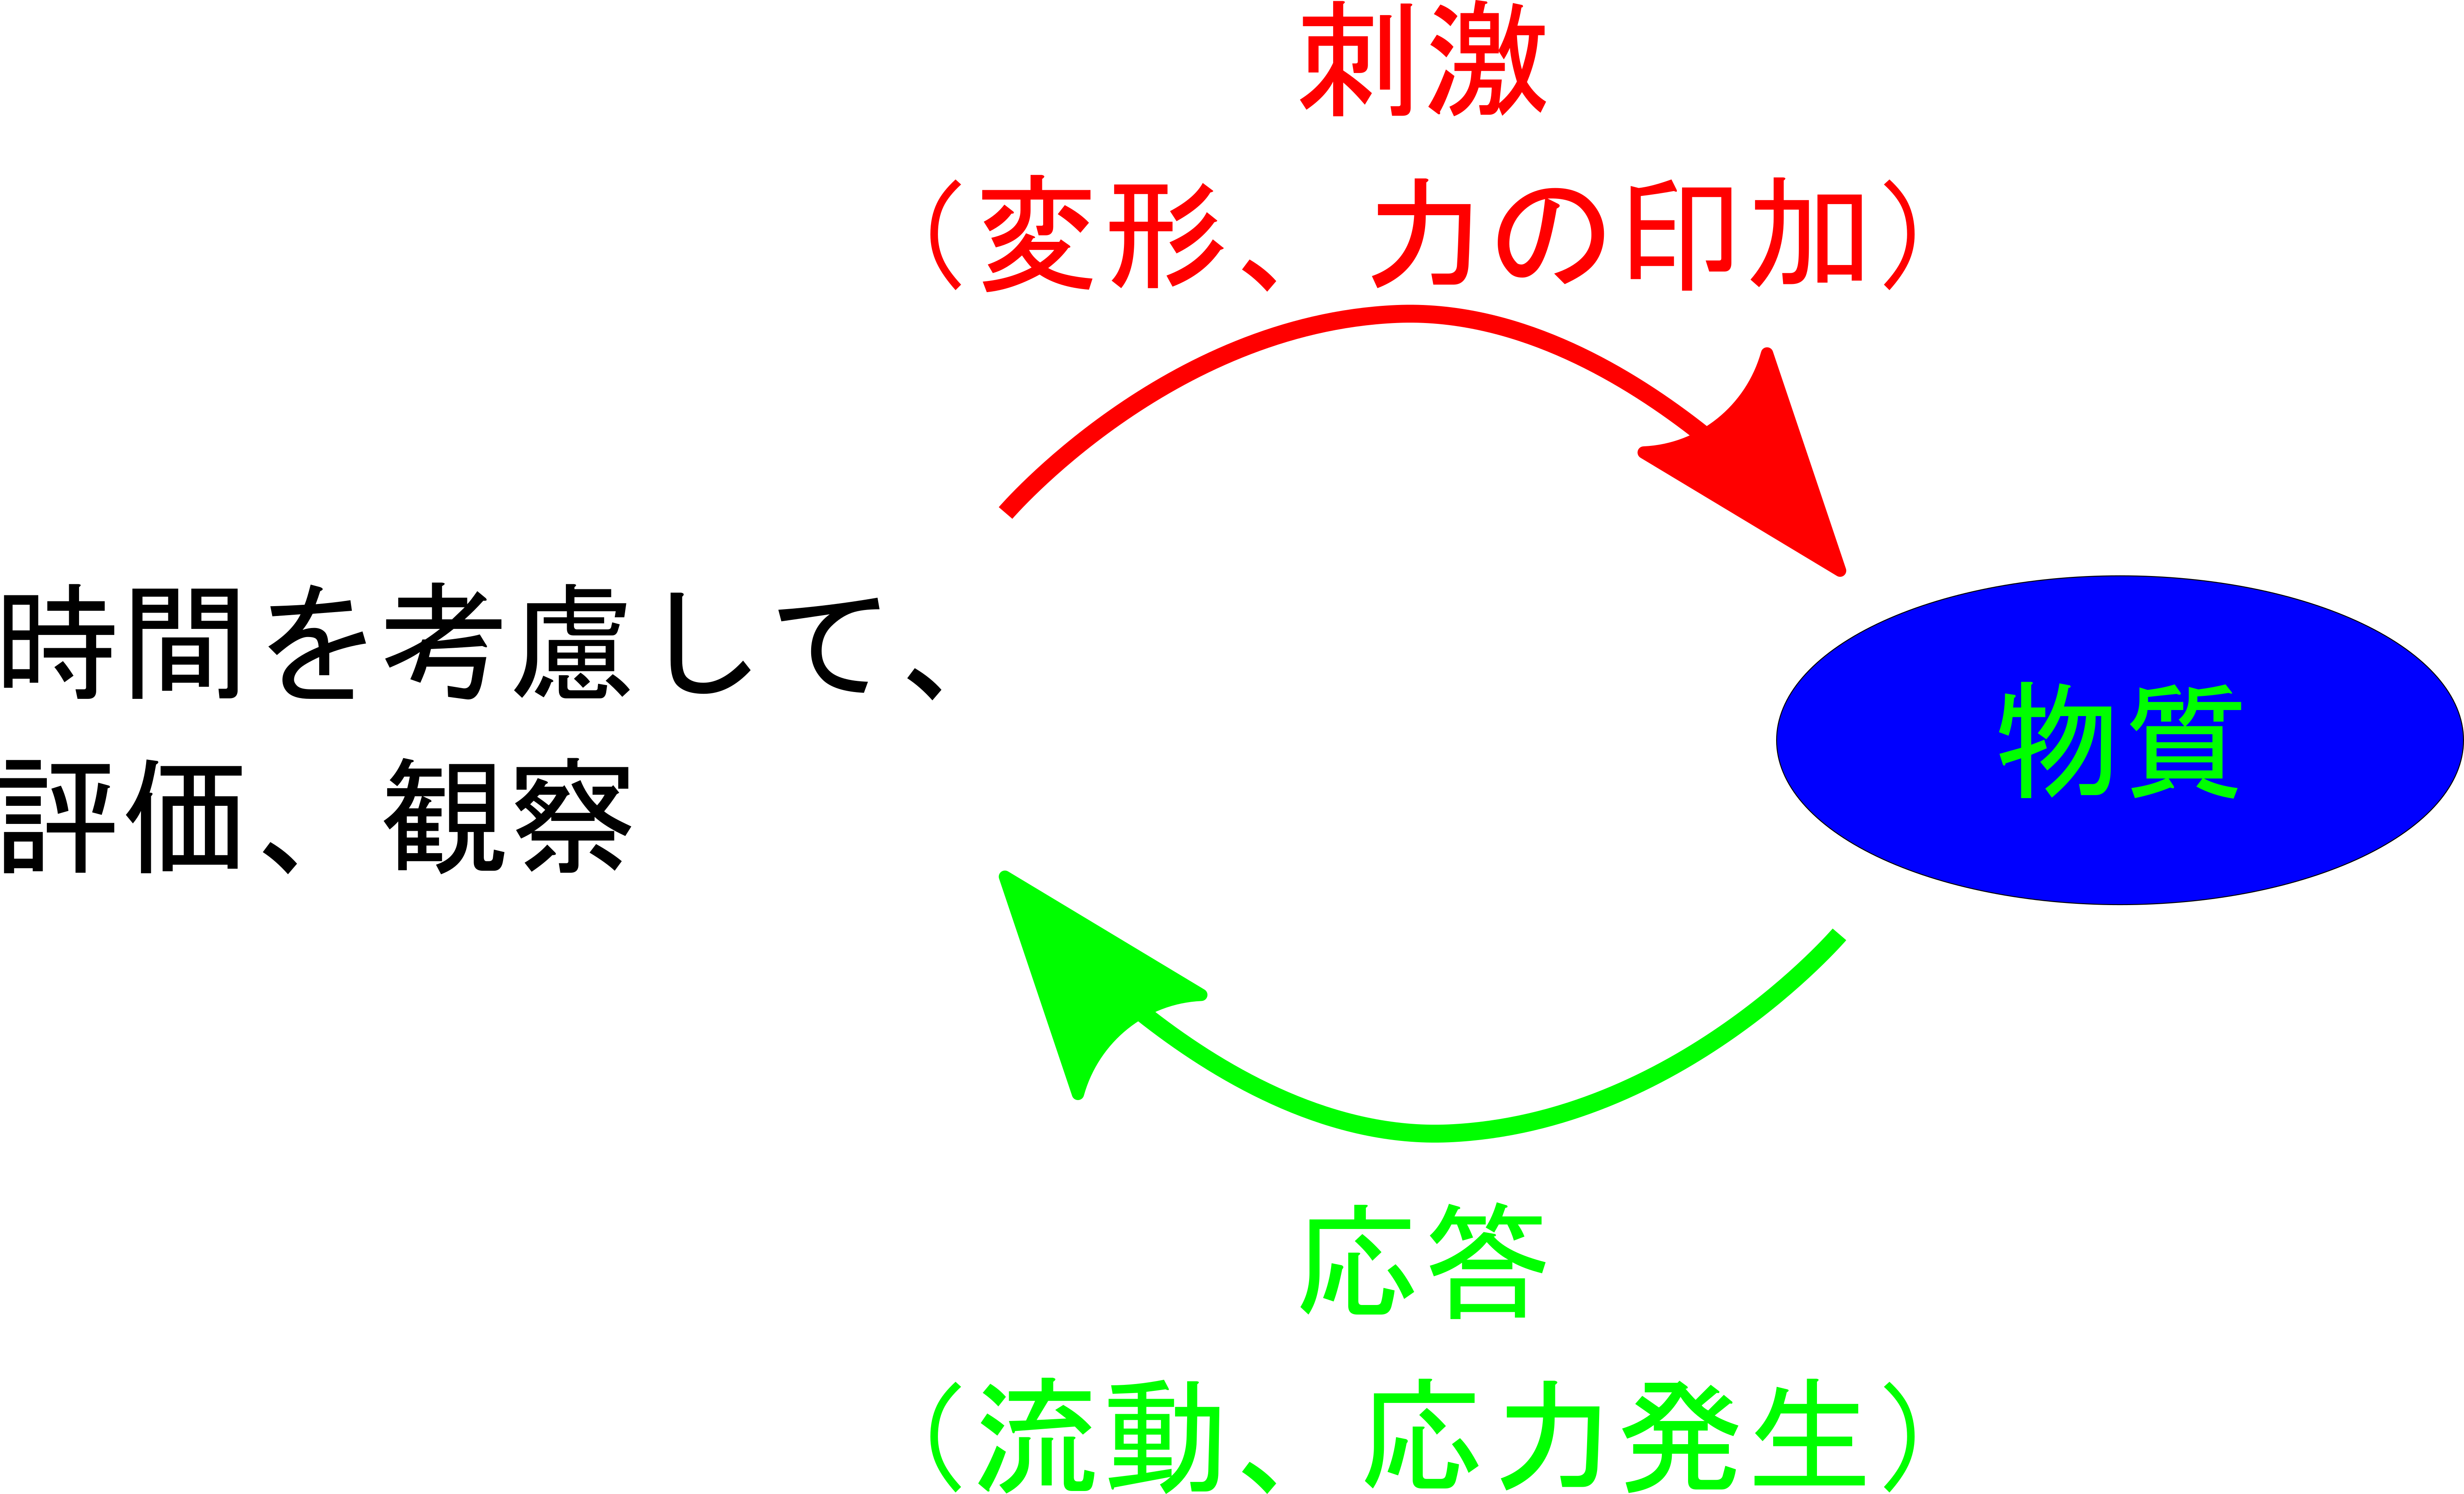
\includegraphics[width=\textwidth]{Rheo_method.png}
		\end{minipage}
		\begin{minipage}{.45\textwidth}
			\large
			\begin{itembox}[l]{レオロジーのやり方}
				\begin{itemize}
					\item 力学的な刺激
					\begin{itemize}
						\item 外力による物質変形
					\end{itemize}
					\item 変形の結果として
					\begin{itemize}
						\item 内部で応力が発生
						\item 流動が生じる場合も
					\end{itemize}
				\end{itemize}
			\end{itembox}
		\end{minipage}
	\caption{レオロジーのやりかた}
	\label{yarikata2}
    \end{center}
\end{figure}

ここでは、わかり易い例として、物質の力学的なレオロジー評価を考えてみましょう。
物質に力学的な刺激を与えるということは、「外力によって物質を変形」させるということに対応します。
このとき、変形の結果として「物質の内部で応力」という応答が生じ、また、流動が生じる場合もあります。

\subsection{力について}
まず、刺激の源となる「力\index{ちから@力}」というものについての確認から始めていきましょう。

力は以下のように定義されています。
そして、その対象となるものの状態に応じて、「静力学\index{せいりきがく@静力学}」と「動力学\index{どうりきがく@動力学}」の2つに分けて考えることができます。
\large
	\begin{itembox}[l]{力の定義}
		「物体の状態を変化させる原因となる作用で、その作用の大きさを表す物理量」
		\begin{itemize}
			\item 静力学
			\begin{itemize}
				\item 静的状態(時間によって系の位置が変化しない状態)に働く力に関して、
				\item 主として、力の釣り合い\index{ちからのつりあい@力の釣り合い}を議論。
			\end{itemize}
			\item 動力学
			\begin{itemize}
				\item 運動量の変化を伴う質点の移動について議論し、
				\item 相互作用する物体系の運動について議論。
			\end{itemize}
		\end{itemize}
	\end{itembox}
\normalsize

この章でのお話としては、まずは、力の釣り合いを取り扱う静力学としてのアプローチから始めていきます。

\subsection{物質の変形と仕事}

静的な釣り合いとして物質に力\index{ちから@力}を加えることを考えた場合、物質の外から加えた力を「外力\index{がいりょく@外力}」と呼び、そして物質の内部に外力に抵抗する力として「内力\index{ないりょく@内力}」が生じます。
このとき、外力と内力が釣り合うという、「作用・反作用の原理」が成り立ちます。
\large
	\begin{itembox}[l]{静的な釣り合いとしての力}
		\begin{itemize}
			\item 物質の外から加えた力を外力として、
			\item 物質の内部に、外力に抵抗する力として内力が生じ、
			\item 外力と内力が釣り合う。$\Leftrightarrow$ 「作用・反作用の原理」
		\end{itemize}
	\end{itembox}
\normalsize

同時に、外力に対応して、物質は変形します。
この釣り合いのもとでの物質の変形も、仕事となります。
この場合、外力が物質の内部に蓄積された(弾性)エネルギーに相当する量の仕事を行ったと考える事ができます\footnote{
	仕事という概念については、次の第 4 章で議論を進めますので、少しお待ち下さい。
}。


\section{弾性体の力学的な刺激と応答}

この節では、わかり易い例として最も単純な固体のモデルである弾性体\index{だんせいたい@弾性体}を対象として、力学的な刺激と応答ということについて、考えていきます。
なお、弾性体という考え方は、変形を受けてもその起源となる外力を除去すれば、全く元の状態に戻るような性質をあらわしています。
さらに、簡単のために時間の因子も除いて考えることにします。

\subsection{物質のひずみ\index{ひずみ@ひずみ}と応⼒}
ここでは、力学的な刺激として、「外力による物質の変形」を考え、その応答として、「内部での応力発生」を考えます。
% 実際には、変形させるために外力と呼ばれる力を物質に与えるわけですが、そのあたりの細かいことは一旦無視しましょう。

外力\index{がいりょく@外力}を与えた結果として変形が生じたとき、物質はひずみ、内部で応力\index{おうりょく@応力}が発生します。
\large
	\begin{center}
		\begin{minipage}{0.38\textwidth}
			\begin{itembox}[l]{外力による物質の変形}
				\begin{itemize}
					\item 引張変形
					\item せん断変形
				\end{itemize}
			\end{itembox}
		\end{minipage}
		\begin{minipage}{0.38\textwidth}
			\begin{itembox}[l]{変形の結果として}
				\begin{itemize}
					\item 物質はひずむ
					\item 内部で応力が発生
				\end{itemize}
			\end{itembox}
		\end{minipage}
	\end{center}
\normalsize

\subsection{二つの変形とひずみ}
変形を考えていくために、まず、物質を一つの軸に沿って引き伸ばす「引張変形\index{ひっぱりへんけい@引張変形}」とトランプのカードを横にずらしたような「せん断変形\index{せんだんへんけい@せん断変形}」の
二つに、変形を単純化します。

この「せん断変形」のイメージが湧きにくいかもしれません。
たとえば、紙をハサミで切るときにそれぞれの刃が向かい合う方向に移動して紙に力を与えているような状況を想像していただければと思います。
このように互い違いの方向に同じ大きさの力が作用することを、偶力\index{ぐうりょく@偶力}と呼びます。
「せん断変形」は、偶力が働いた結果として生じる変形であると理解してください。

\subsubsection{伸張ひずみ\index{しんちょうひずみ@伸張ひずみ}}
引張変形に対応する物質のひずみを記述する最も単純なものが、棒状のものを一方向にだけ変形させたときのコーシーひずみ(図 \ref{causy})になります。
このとき、変形量を変形前の長さで除したものがひずみ (一般に、コーシーひずみのような伸張ひずみはギリシア文字の $\varepsilon$ と表記) となります。
\begin{figure}[htb]
	\begin{center}
		\begin{minipage}{0.45\textwidth}
			\large
			\begin{itembox}[l]{コーシーひずみ:}
				\vspace{-3mm}
				\begin{align*}
					\varepsilon_c &= \dfrac{\text{\textbf{変形量}}}{\text{\textbf{変形前の長さ}}} \\
					&=\dfrac{\Delta L}{L_0} = \dfrac{L-L_0}{L_0}
				\end{align*}
			\end{itembox}
		\end{minipage}
		\begin{minipage}{0.45\textwidth}
			\begin{center}
				\includegraphics[width=0.9\textwidth]{Causy.png}
			\end{center}
		\end{minipage}
		\caption{コーシーひずみ}
		\label{causy}
	\end{center}
\end{figure}

\subsubsection{せん断ひずみ\index{せんだんひずみ@せん断ひずみ}}
また、せん断変形\index{せんだんへんけい@せん断変形}によるひずみ (せん断ひずみはギリシア文字の $\gamma$ と表記) は、図 \ref{shear} に示したように、変形方向への変形量をサンプルの厚みで除した形で表すことになります。
このとき、高さ $h$ を一定とし、変形前後での体積変化もないものと考えています。
\begin{figure}[htb]
	\begin{center}
		\begin{minipage}{0.45\textwidth}
			\large
			\begin{itembox}[l]{せん断ひずみ:}
				\vspace{-3mm}
				\begin{align*}
					\gamma &= \dfrac{\text{\textbf{変形方向への変形量}}}{\text{\textbf{サンプルの厚み}}} \\
					&=\dfrac{x}{h}
				\end{align*}
			\end{itembox}
		\end{minipage}
		\begin{minipage}{0.45\textwidth}
			\begin{center}
				\includegraphics[width=0.9\textwidth]{Shear.png}
			\end{center}
		\end{minipage}
		\caption{せん断ひずみ}
		\label{shear}
	\end{center}
\end{figure}

なお、ひずみは、長さを長さで割ったものとなりますので、次元を持たない無次元量であることに注意してください。

\subsection{応力のイメージ}
応力\index{おうりょく@応力}とは、物質の内部に生じている力の大きさを表す物理量であり、その表す意味は単位面積あたりに働く内部の力ということになります。
したがって、その次元は以下のように書けます。
\large
	\begin{itembox}[l]{応力の次元}
		\vspace{-3mm}
		\begin{align*}
			[\text{応力}] = \dfrac{[\text{力}]}{[\text{面積}]} = \dfrac{[\mathrm{N}]}{[\mathrm{m}]^2} = [\mathrm{Pa}]
		\end{align*}
	\end{itembox}
\normalsize

棒状の物質に引っ張り変形を与えた場合の、外力と応力のイメージを図 \ref{stress} に示しました。
このとき、棒の長手方向にはどの位置で切断したとしても、同一の応力が働いていることに注意してください。
\begin{figure}[htb]
	\begin{center}
		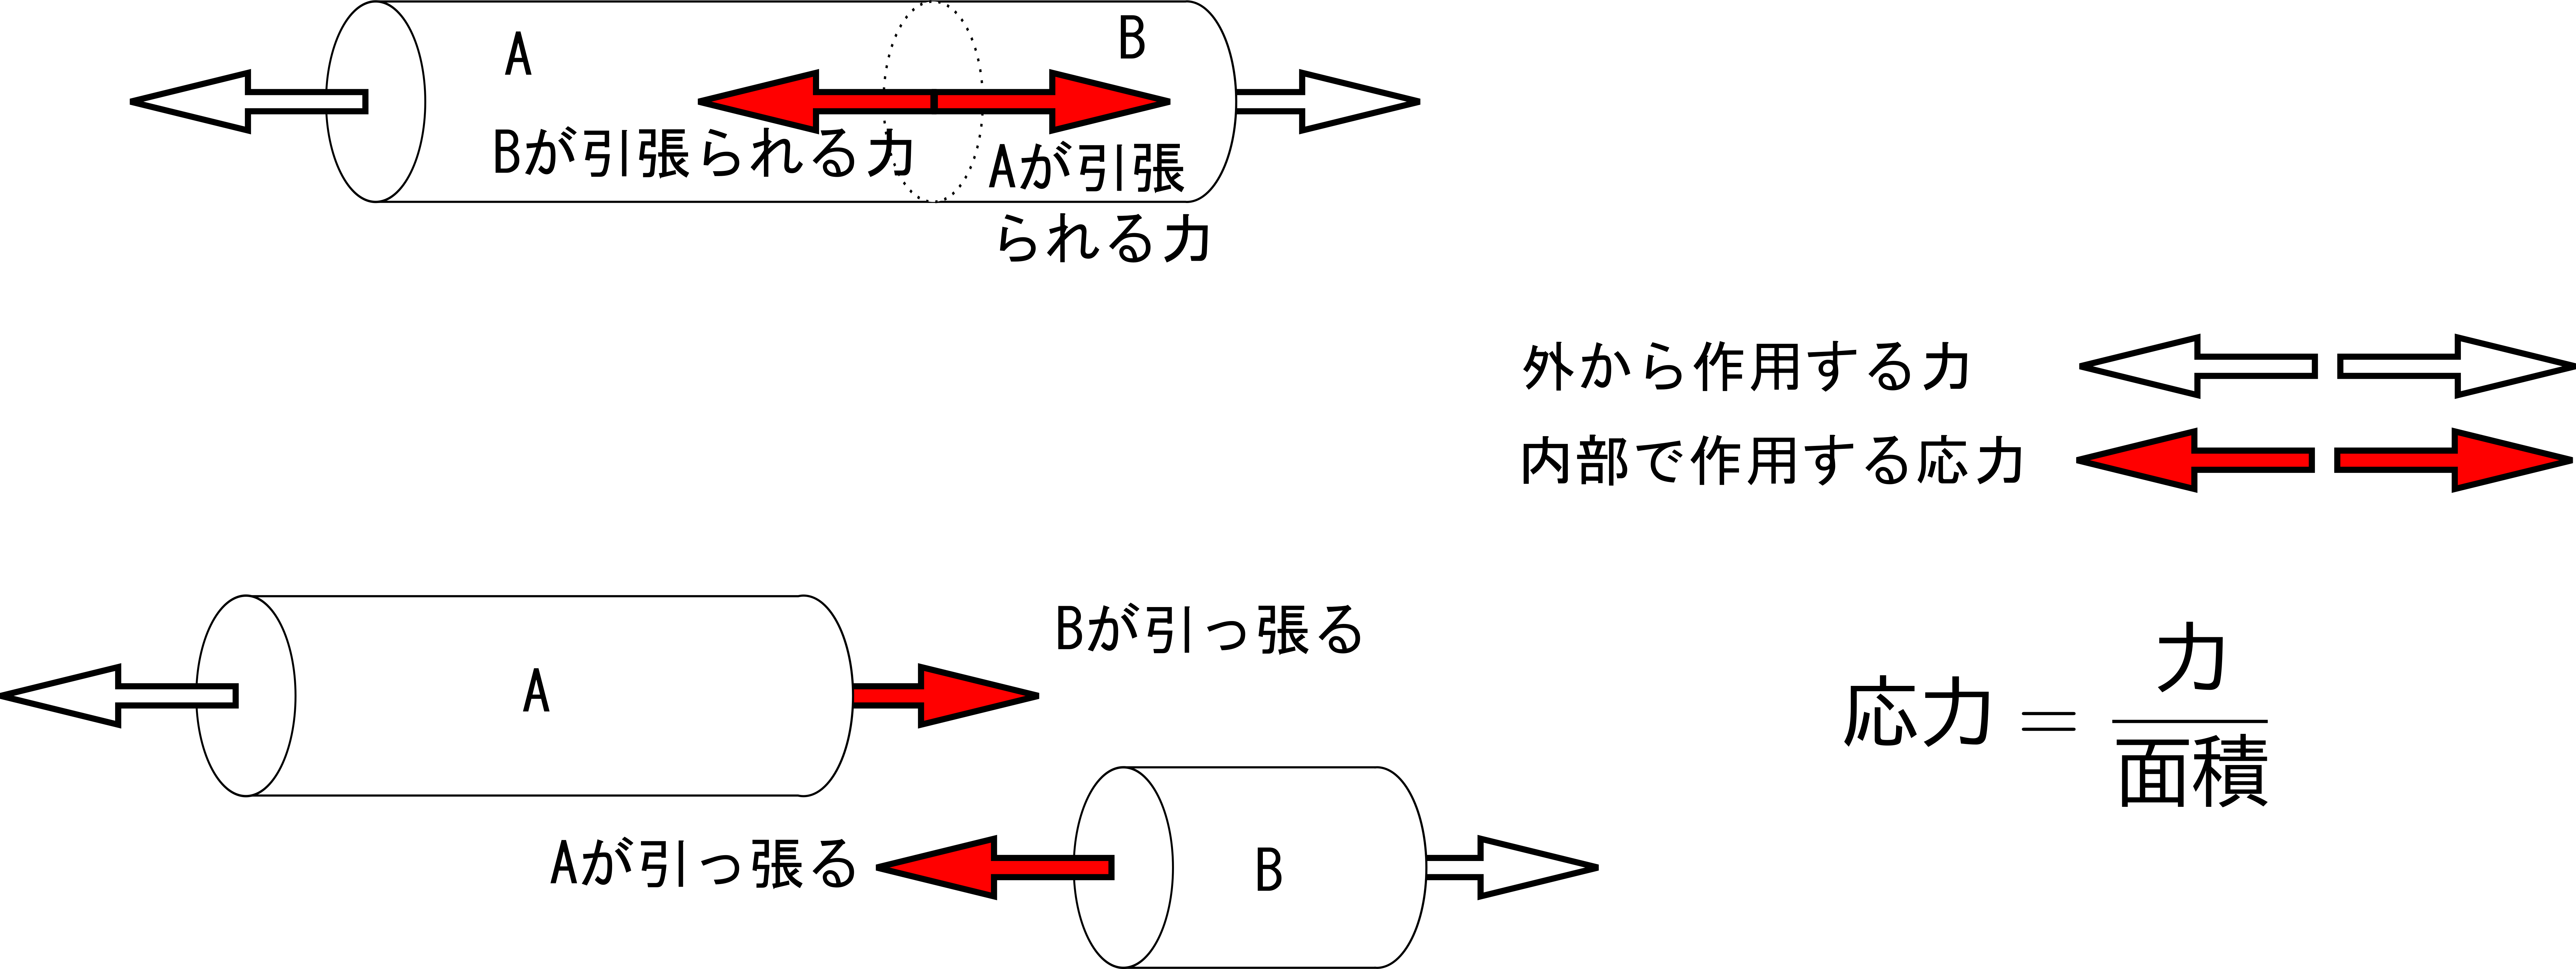
\includegraphics[width=.9\textwidth]{Stress.png}
		\caption{応力のイメージ}
		\label{stress}
	\end{center}
\end{figure}

\subsubsection{伸長応力\index{しんちょうおうりょく@伸長応力} $\sigma$}
伸長時に働く応力は、一般に、ギリシア文字の $\sigma$ と表記します。
表式とすれば、以下のように書くことができます。
\begin{align*}
	\sigma = \dfrac{F}{A}
\end{align*}
なお、$F$ は外部から加えた外力を、$A$ は内部で応力が働く断面積ということになります。

繰り返しますが、応力は単位面積あたりに働く内部の力ですから、図 \ref{elong_stress} に示したように細い棒と入れ替えて断面積が小さくなれば、それに反比例して応力は増加します。
\begin{figure}[htb]
	\begin{center}
		\begin{minipage}{0.45\textwidth}
			\large
			\begin{align*}
				\sigma &= \dfrac{\text{\textbf{与えた力}}}{\text{\textbf{断面積}}} \\
					&=\dfrac{F}{A}
			\end{align*}
			\begin{itemize}
				\item $F$ は外部から加えた外力
				\item $A$ は内部で応力が働く断面積
			\end{itemize}
			\begin{itembox}[l]{同一の外力でも}
				\begin{itemize}
					\item 断面積が小さくなれば、
					\item 反比例して応力は増加
				\end{itemize}
			\end{itembox}
		\end{minipage}
		\begin{minipage}{0.45\textwidth}
			\begin{center}
				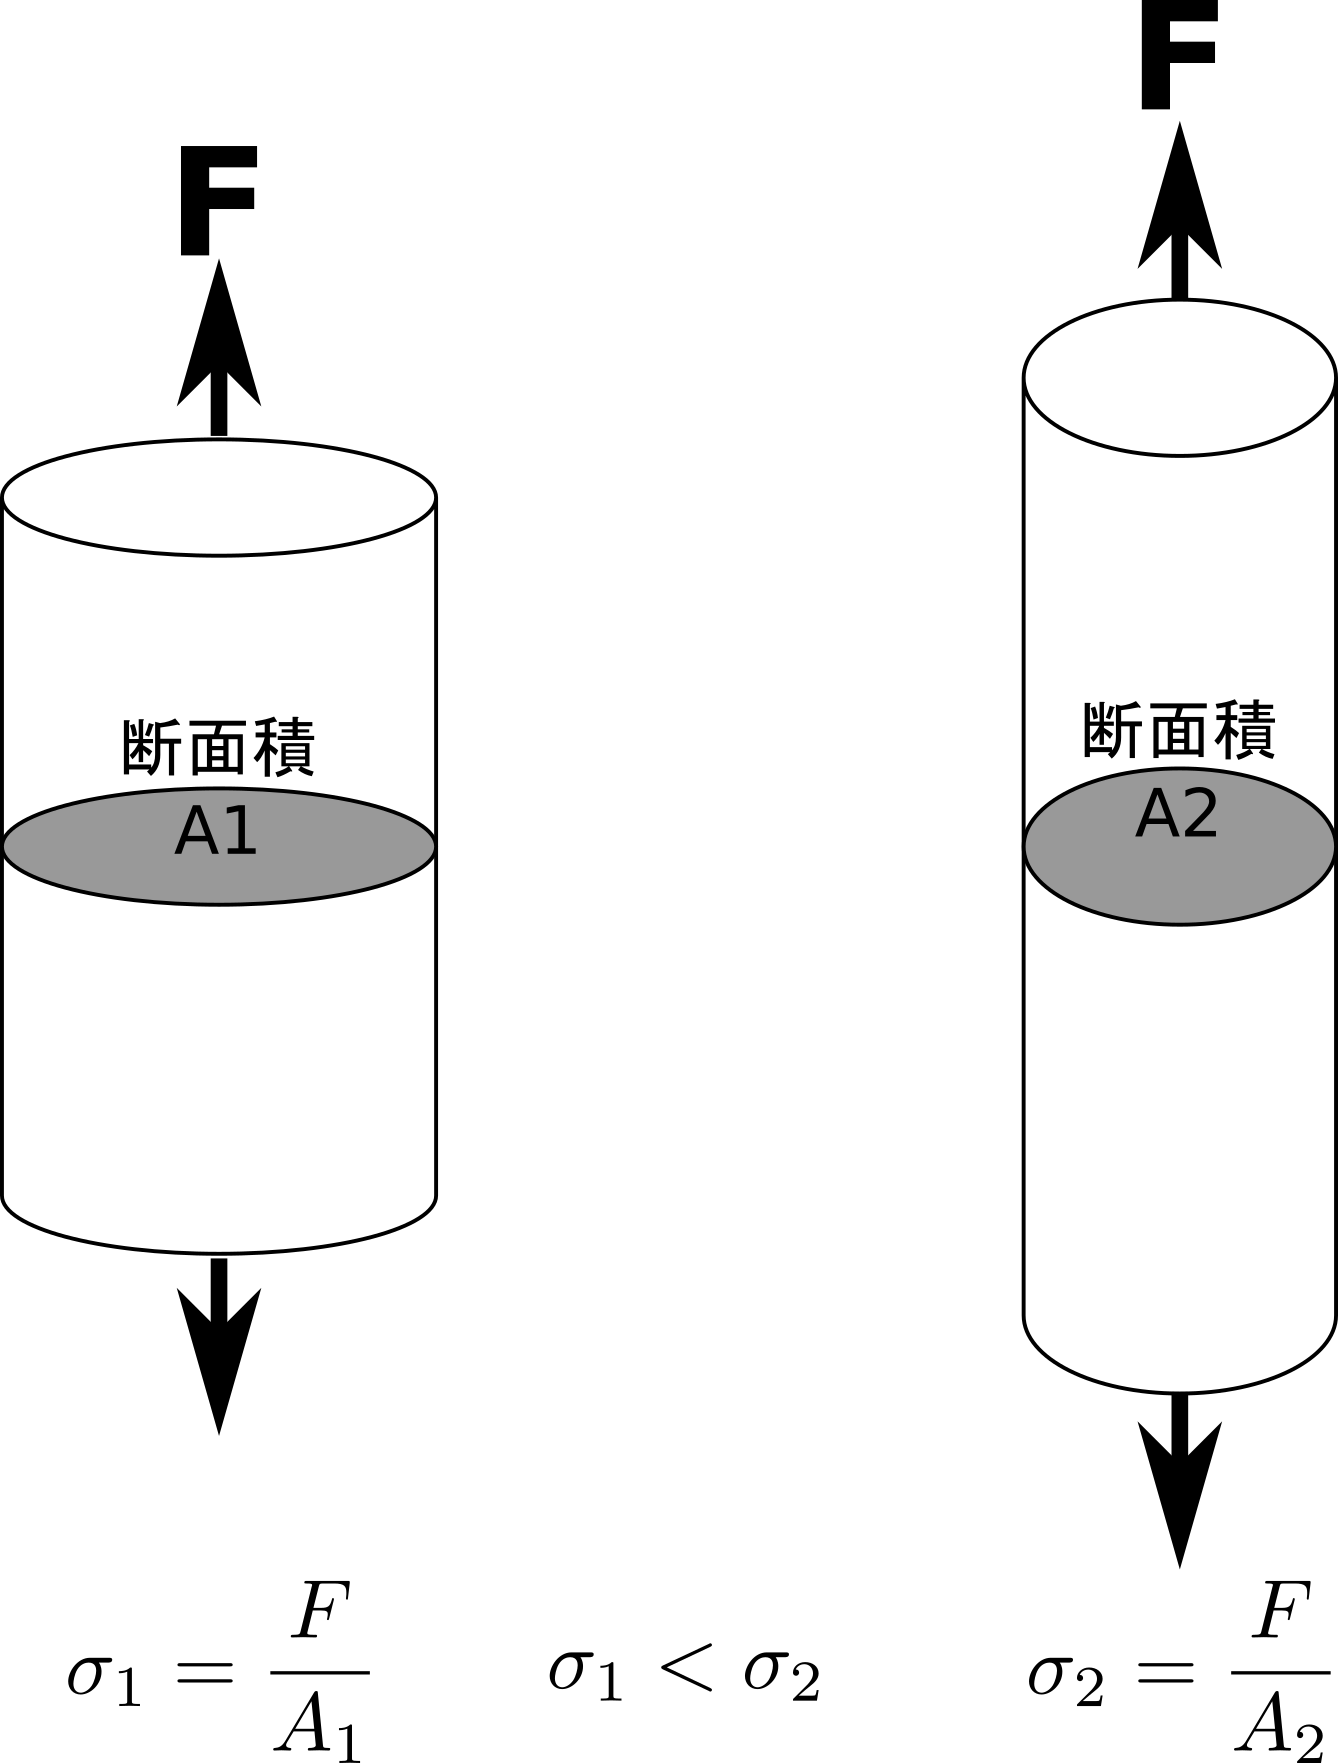
\includegraphics[width=.8\textwidth]{elong_stress.png}
			\end{center}
		\end{minipage}
		\caption{伸長応力}
		\label{elong_stress}
	\end{center}
\end{figure}

\subsubsection{せん断応力 $\tau$}
互いに向かい合う同じ大きさの力である偶力 $F$ を作用させてせん断変形\index{せんだんへんけい@せん断変形}を生じた場合のせん断応力\index{せんだんおうりょく@せん断応力}(せん断の場合は、応力を $\tau$ と表記)のイメージを、図 \ref{shear_stress} に示しました。
なお、力を働かせた上面の面積が $A$ であることに注意してください。
\begin{figure}[htb]
	\begin{center}
		\begin{minipage}{0.45\textwidth}
			\large
			\begin{itembox}[l]{せん断応力 $\tau$}
				\vspace{-3mm}
				\begin{align*}
					\tau &= \dfrac{\text{\textbf{与えた力}}}{\text{\textbf{働かせた面積}}} \\
					&= \dfrac{F}{A}
				\end{align*}
			\end{itembox}
		\end{minipage}
		\begin{minipage}{0.45\textwidth}
			\begin{center}
			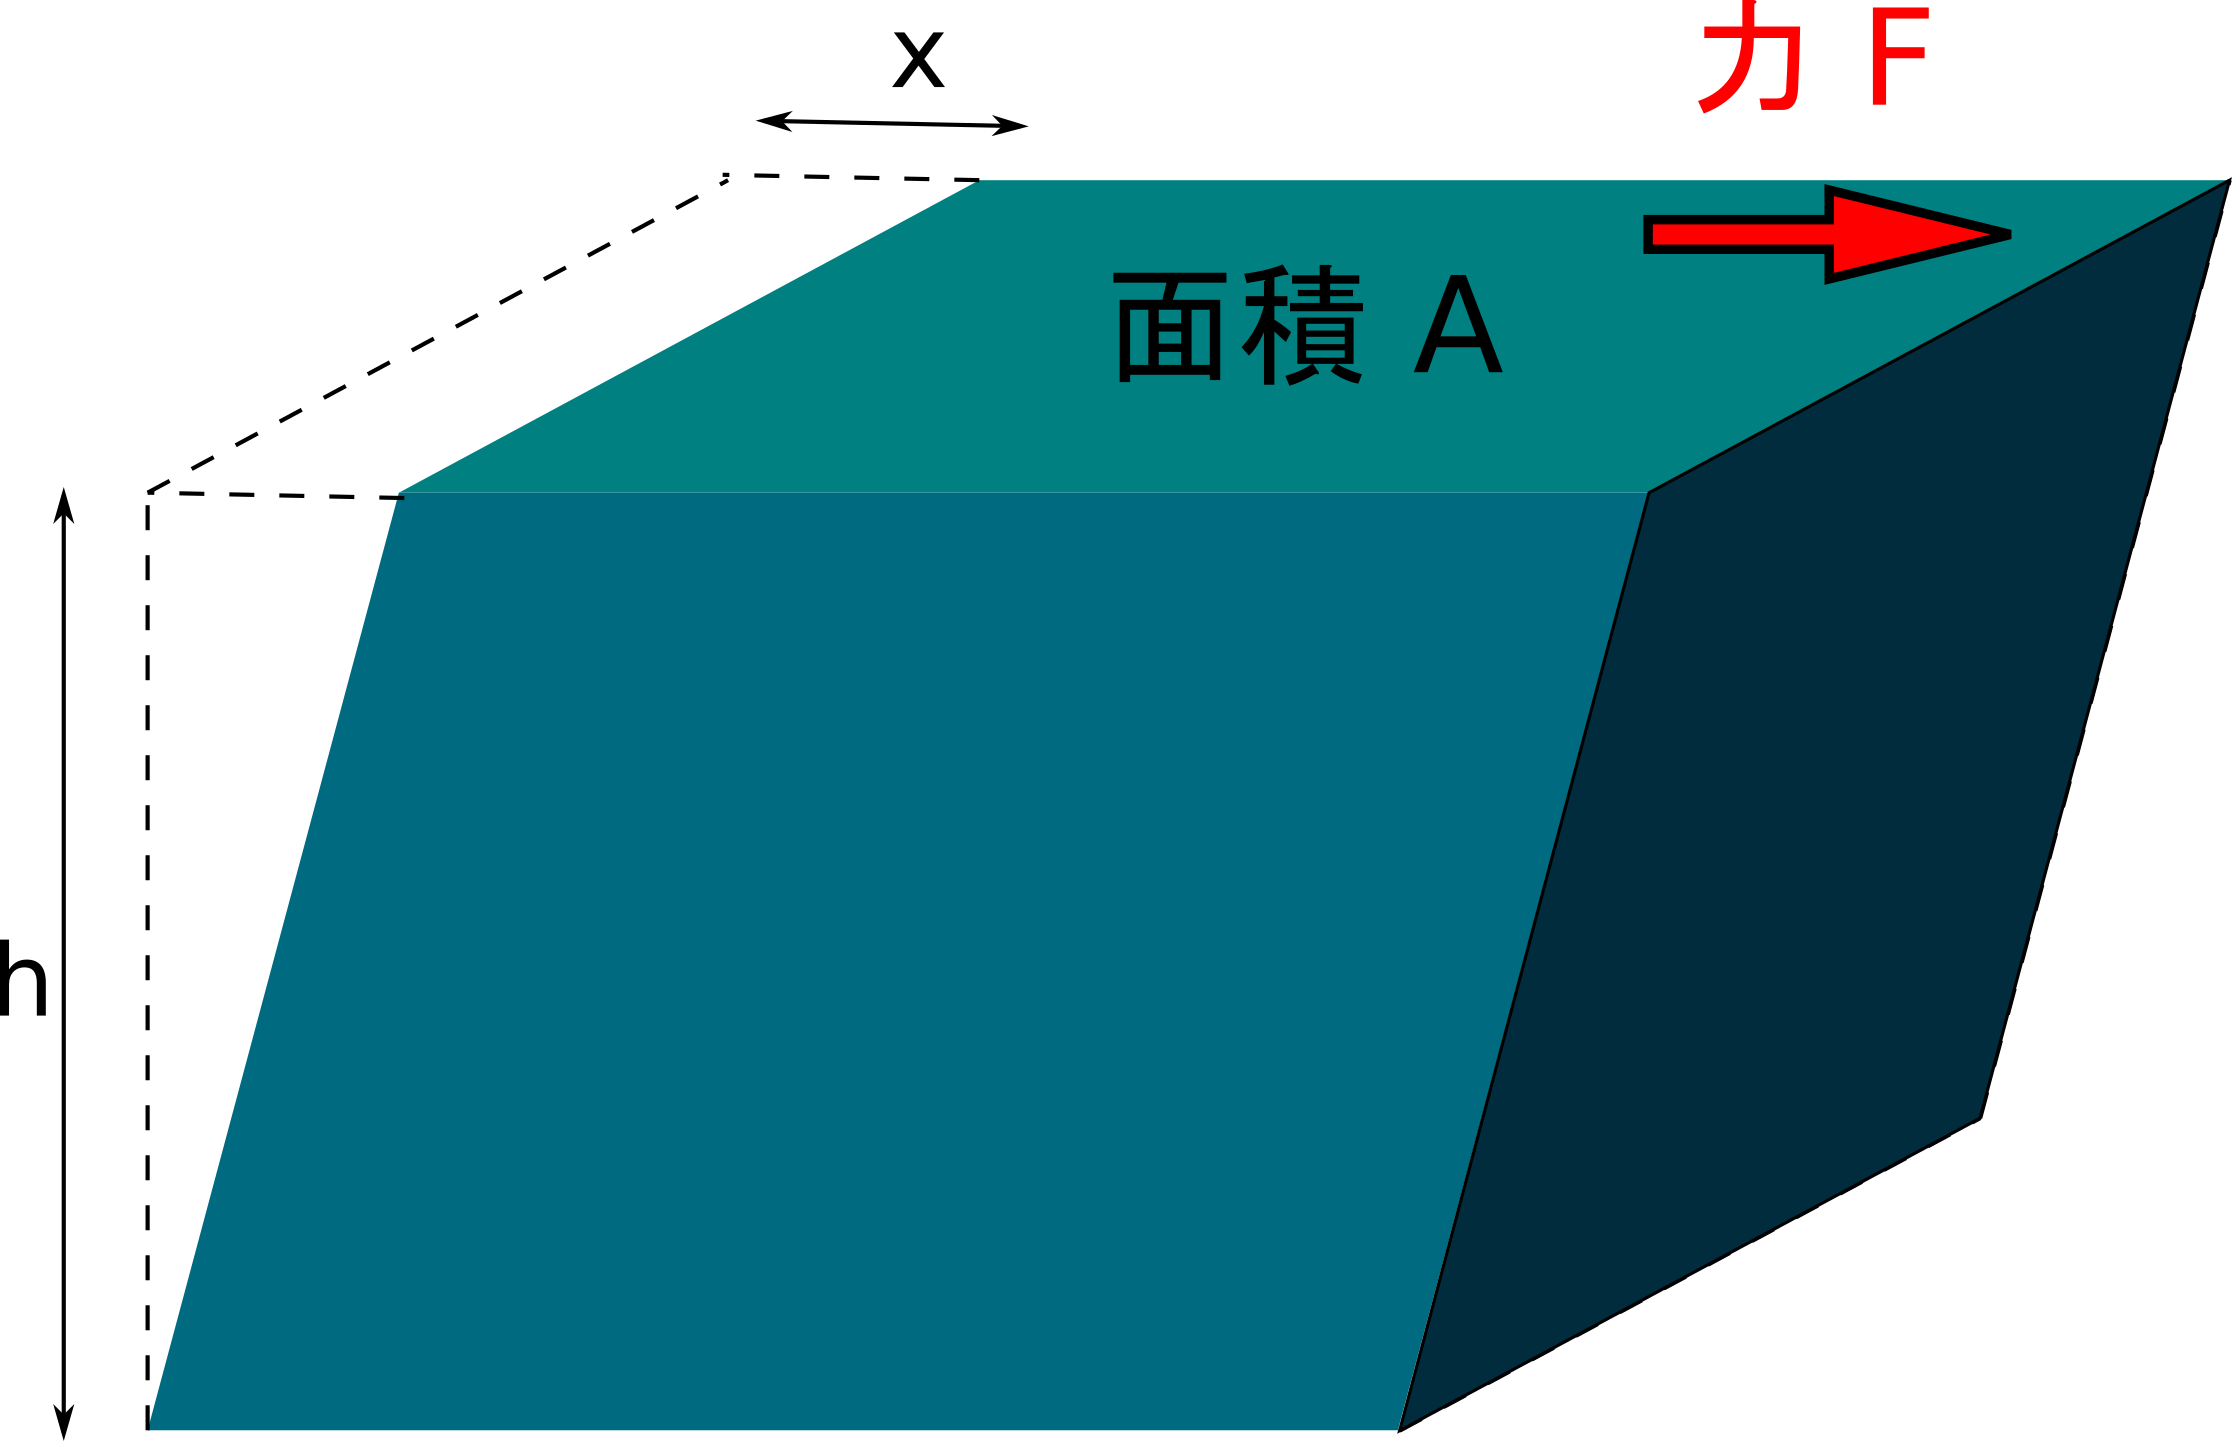
\includegraphics[width=.9\textwidth]{shear_2.png}
			\end{center}
		\end{minipage}
		\caption{せん断応力}
		\label{shear_stress}
	\end{center}
\end{figure}

このとき、サンプルの厚さ方向には、どの位置であっても同一のせん断応力\index{せんだんおうりょく@せん断応力}が作用していることになり、伸張ひずみの場合と同様に厚さ方向にはどの位置で切断したとしても同一の偶力が作用していることになります。

このせん断応力のイメージは、トランプのカードが重なったデッキを想像することで、理解しやすくなるかもしれません。
つまり、デッキの間に挟まったカードは、一枚上のカードと下のカードによって偶力を受けることになるわけです。
\begin{figure}[htbp]
	\begin{center}
		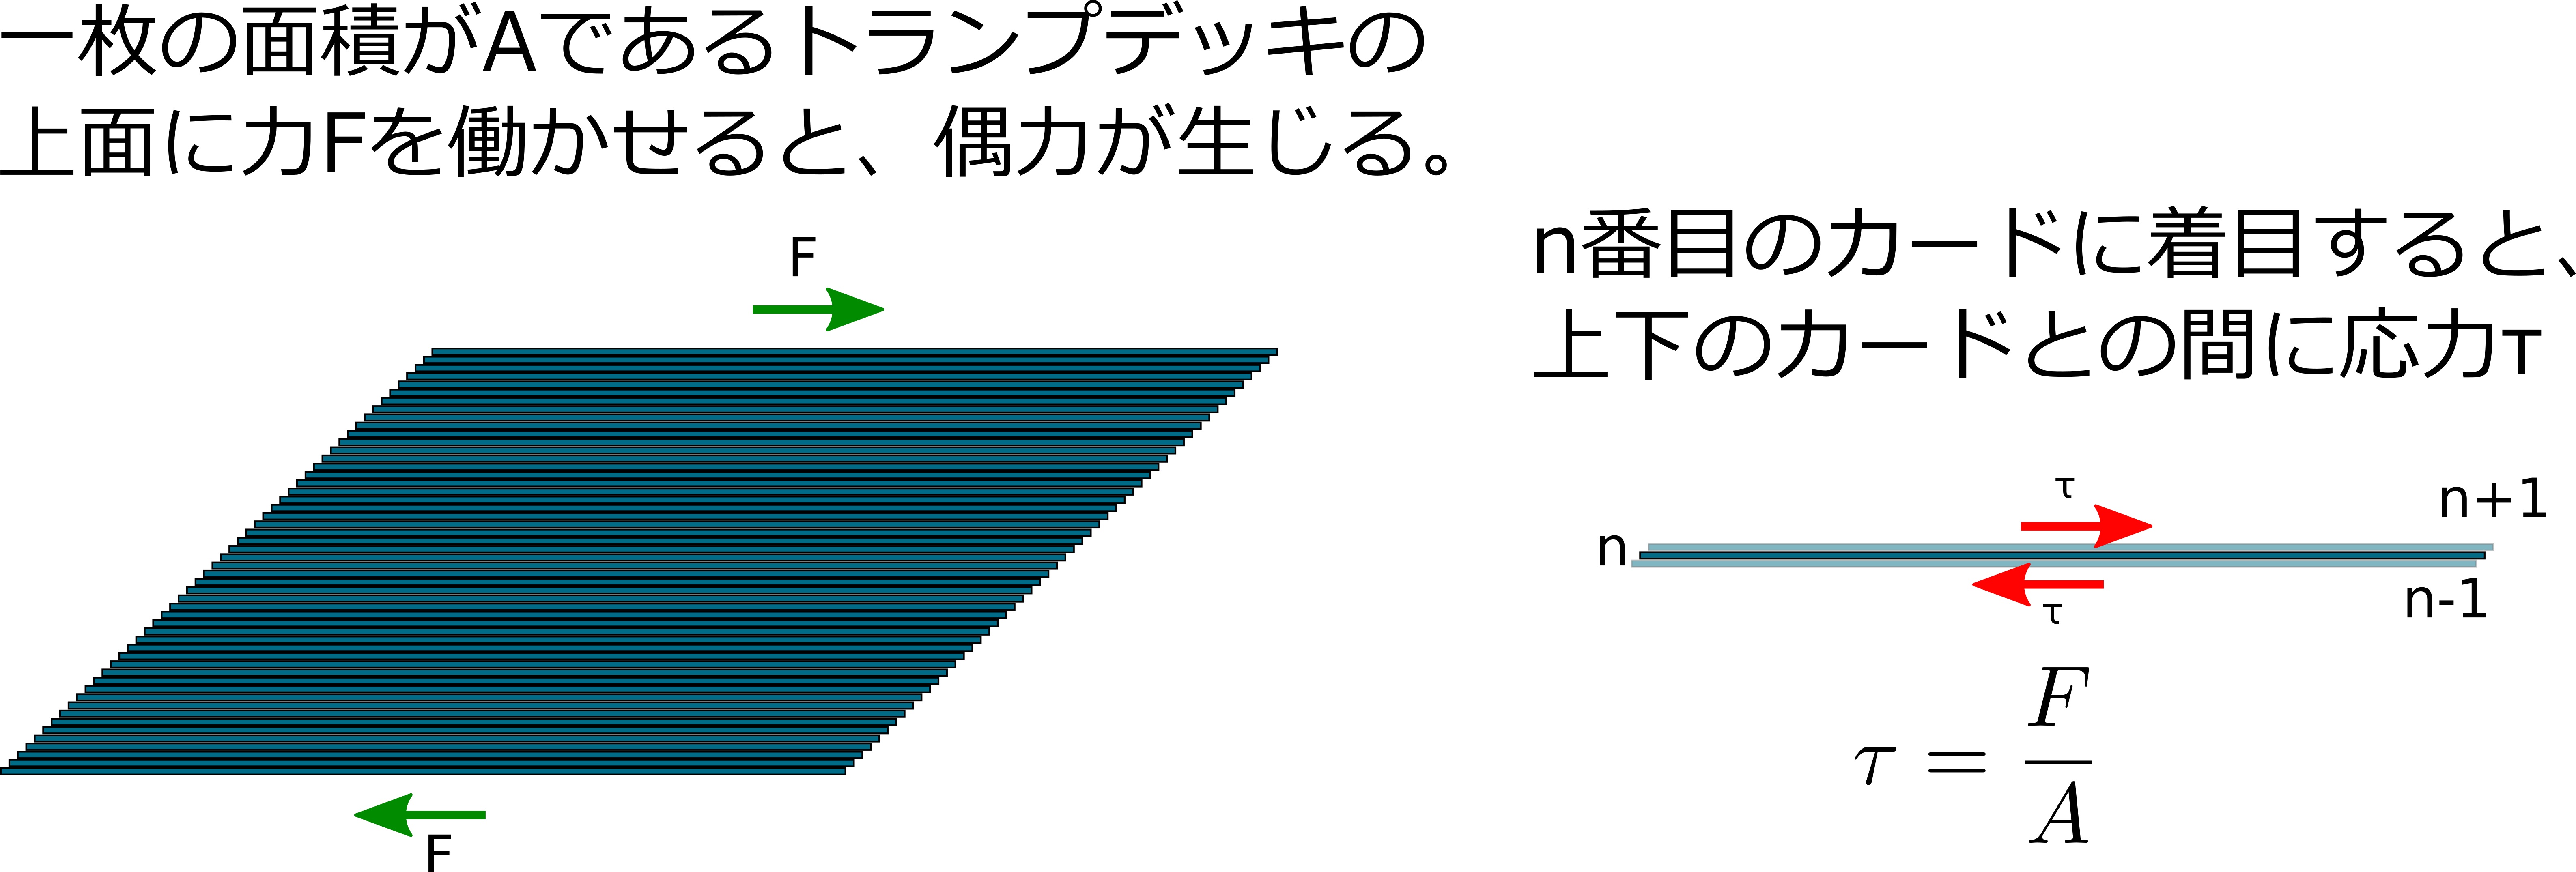
\includegraphics[width=.9\textwidth]{trump_deck.png}
		\caption{内部でのイメージ}
		\label{trump}
	\end{center}
\end{figure}

\section{力学モデルについて}
\subsection{弾性体のモデル}

ここまで刺激と応答の例として使ってきた弾性体を、物質として評価する方法について考えてみましょう。
つまり、弾性体の力学応答を書き表すことが出来るモデルを数式として表すことで、異なる物質を定量的に比較できるようになることを目指すわけです。

\subsubsection{Hooke の法則}

これまでの経験から、弾性体はあたかもバネのように取り扱うことができることが知られています。
そして、バネの力学的な振る舞いには、イギリスの物理学者 Robert Hooke が見出した「Hooke の法則」\index{ふっくのほうそく@Hooke の法則}と呼ばれる以下の関係があることがわかっています。
\begin{figure}[htb]
	\begin{center}
		\begin{minipage}{0.45\textwidth}
			\large
			\begin{itembox}[l]{Hooke の法則}
				\vspace{-3mm}
				\begin{align*}
					\text{外力} &= \text{比例定数} \times \text{変位量} \\[8pt]
					F(x) &= k x
				\end{align*}
			\end{itembox}
		\end{minipage}
		\begin{minipage}{0.45\textwidth}
			\begin{center}
			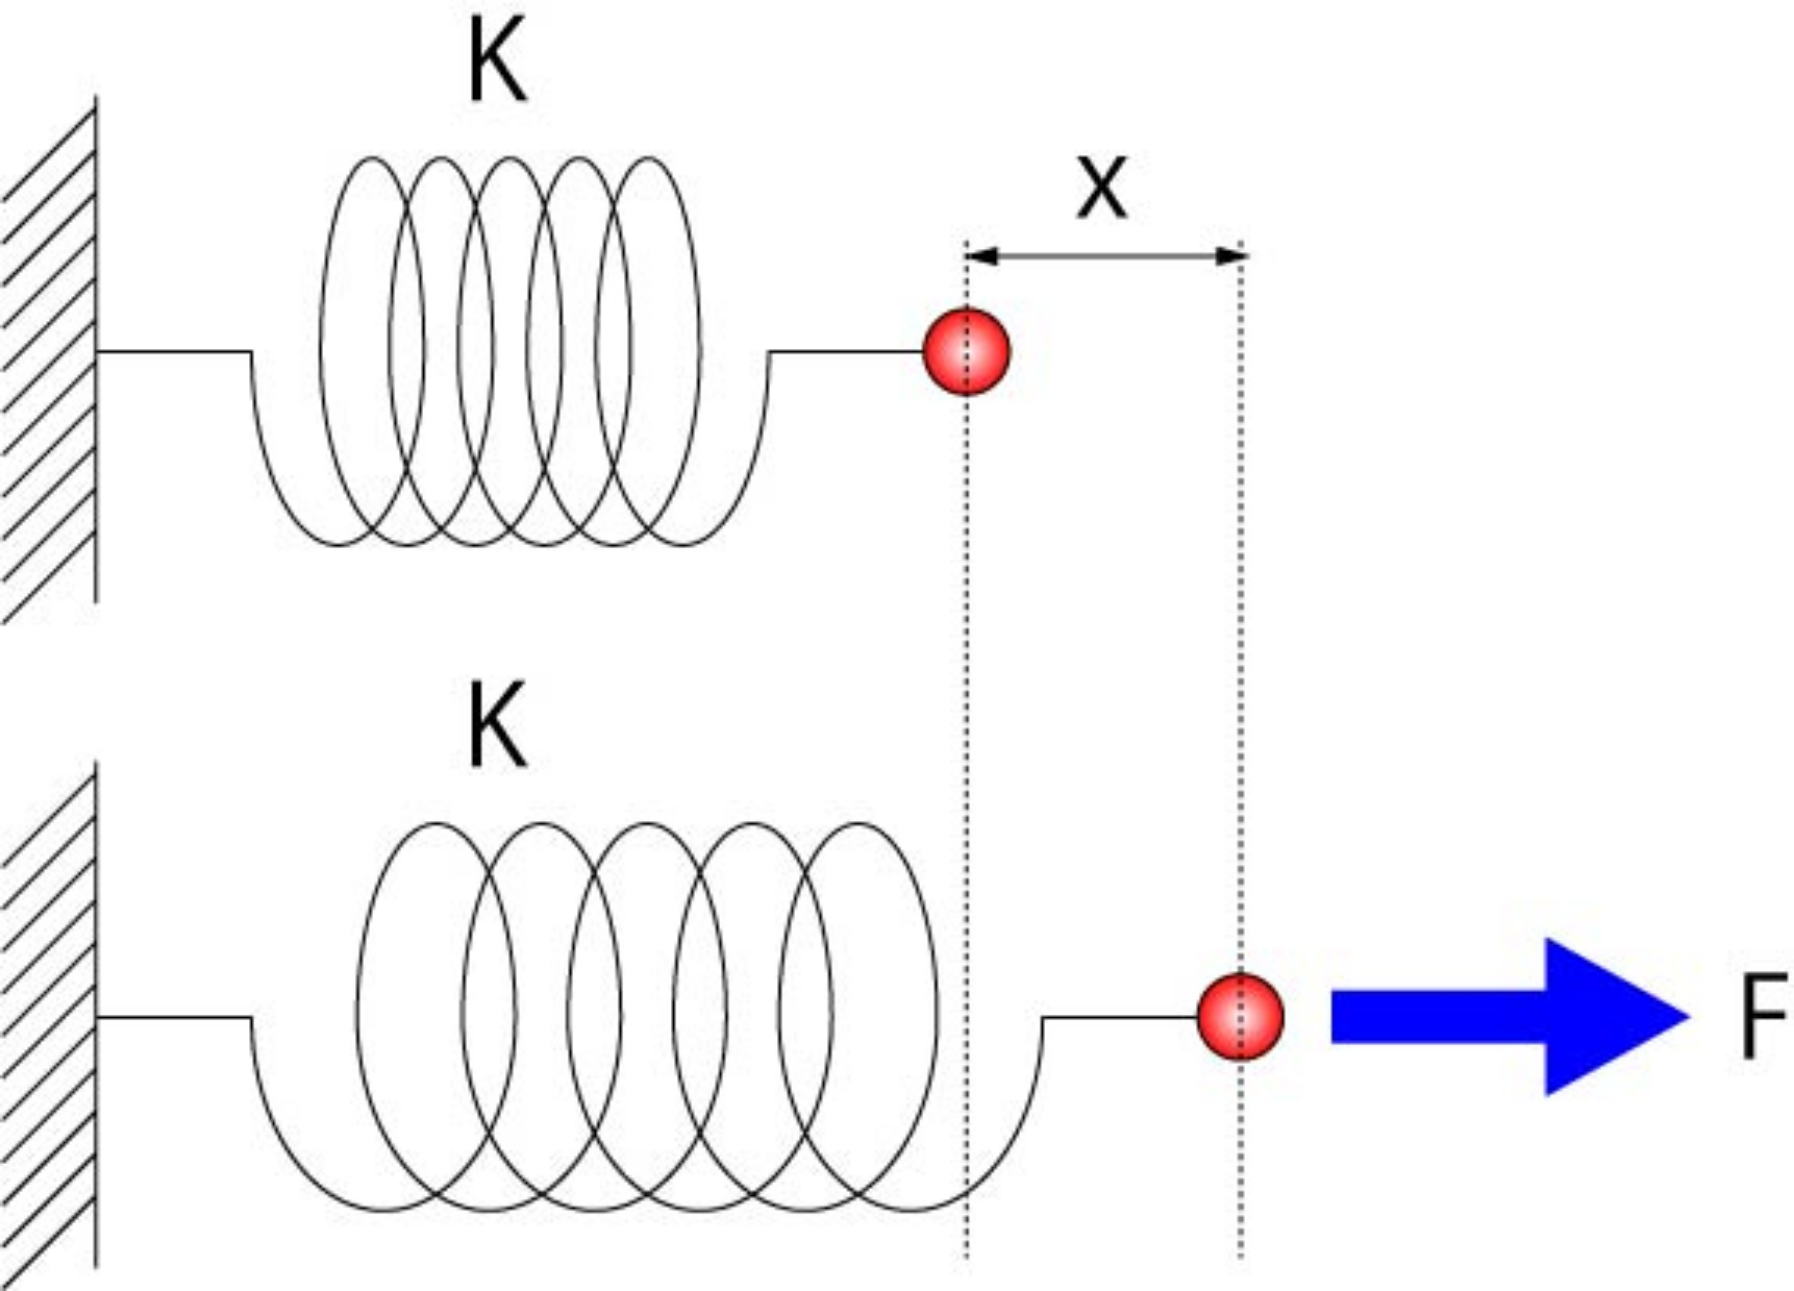
\includegraphics[width=.8\textwidth]{spring.png}
			\end{center}
		\end{minipage}
		\caption{Hooke の法則}
		\label{hook}
	\end{center}
\end{figure}

この式は、外力 $F$ と変位量 $x$ が比例(比例定数が $k$)することを表しています。

\subsubsection{弾性体の力学モデル}

弾性体の力学モデルは、上述のHooke の法則に従う形で、以下のようになります。
\begin{figure}[htb]
	\begin{center}
		\begin{minipage}{0.45\textwidth}
			\large
			\begin{itembox}[l]{弾性体の伸張変形}
				\begin{itemize}
					\item 変形ひずみ $\varepsilon$ と比例して、
					\item 応力 $\sigma$ が生じ、
					\item 比例定数が引張弾性率 $E$
				\end{itemize}
			\end{itembox}
		\end{minipage}
		\begin{minipage}{0.45\textwidth}
			\begin{center}
			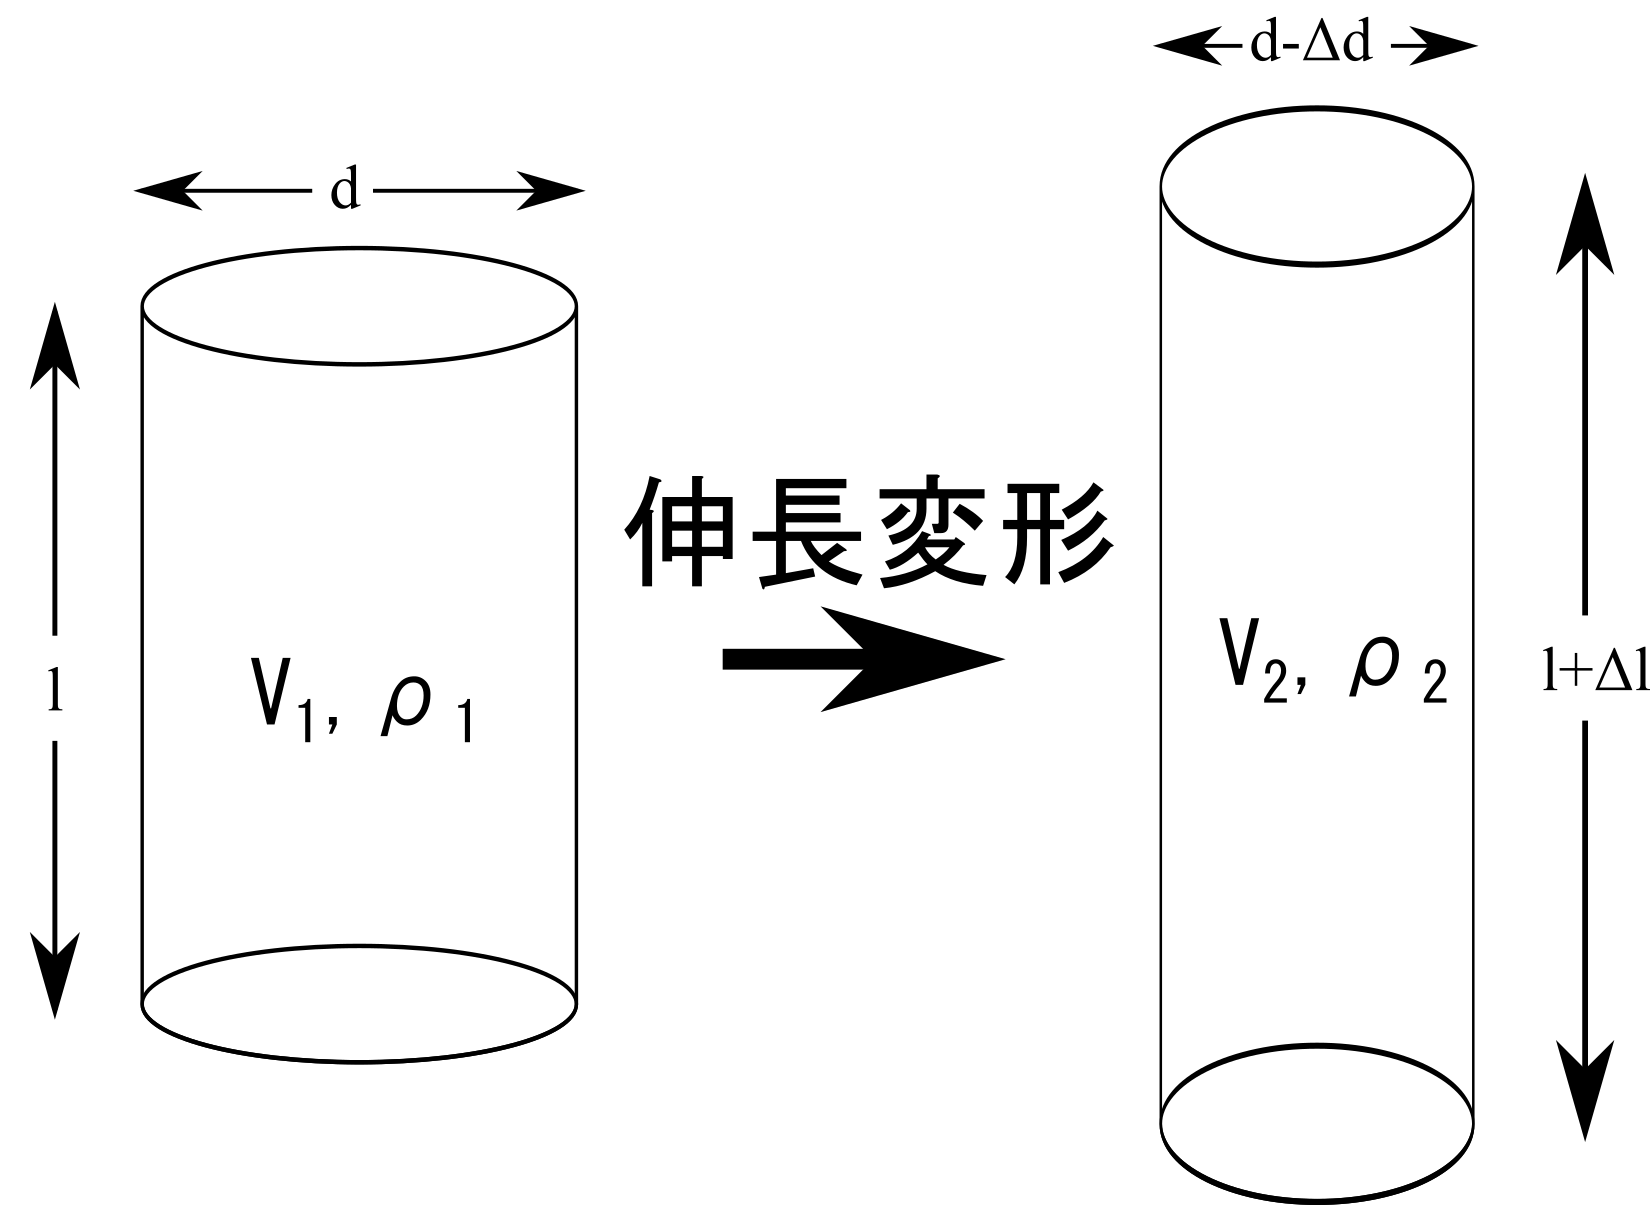
\includegraphics[width=.8\textwidth]{hook_law.png}
			\end{center}
		\end{minipage}
		\caption{弾性体の伸張変形モデル}
		\label{eq:hookian}
	\end{center}
\end{figure}

この関係を表式とすれば、下式となります。
\begin{align}
	\text{伸長応力} &= \text{引張弾性率} \times \text{ヘンキーひずみ} \notag \\
	\sigma &= E \varepsilon 
	\label{eq:hookian2}
\end{align}
なお、ひずみは無次元量でしたから、引張弾性率 $E$ は伸長応力 $\sigma$ と同じ次元である [Pa] となります。

ここで、気をつけていただきたいのは、弾性体の Hooke モデルでは全体のひずみに比例するのは応力であるということです。
何度も繰り返しましたように、応力とは、働いている力を面積で除したものです。
したがって、伸張に伴って変化した面積に対応した応力を考える必要があります。

また、この Hooke モデルは、せん断変形の場合にも使うことができます。
このときは、以下に示したように、
\begin{align}
	\text{せん断応力} &= \text{せん断弾性率} \times \text{せん断ひずみ} \notag \\
	\tau &= G \gamma
\end{align}
せん断変形の場合は、比例定数はせん断弾性率と呼ばれ、$G$ で表され、せん断応力 $\tau$ と同じ次元である [Pa] となります。

\subsection{液体の変形と応答}

ここまでの議論は、固体のモデルとして弾性体を変形の対象として行ってきました。
次に、液体のモデルを考えてみましょう。

\subsubsection{流れるという性質}
液体と固体の違いについては後ほど詳しく議論しますが、ここでは非常に単純に外力によって変形されたら元には戻れない「流れる」という性質を持った物質と考えてください。
この性質を簡単にまとめると以下のようになります。
\begin{figure}[htb]
	\begin{center}
		\begin{minipage}{0.55\textwidth}
			\large
			\begin{itembox}[l]{流れるという性質}
				\begin{itemize}
					\item コップの中ではじっとしている。
					\item 変形を与えると流れる
					\begin{itemize}
						\item 元には戻らない。
						\item 変形を止めれば、応力も消失
					\end{itemize}
					\item 応答を見るのが困難
					\begin{itemize}
						\item 変形を続けながら応力を測る
						\item 液体内部の変形と応力を見積る
					\end{itemize}
				\end{itemize}
			\end{itembox}
		\end{minipage}
		\begin{minipage}{0.35\textwidth}
			\begin{center}
			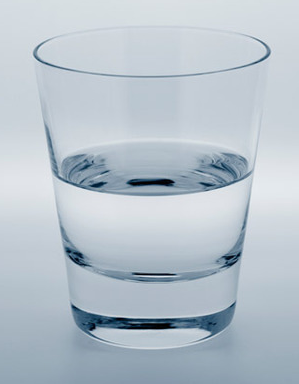
\includegraphics[width=.6\textwidth]{cup_water.png}
			\end{center}
		\end{minipage}
		\caption{流れるという性質}
		\label{fig:flow}
	\end{center}
\end{figure}

この「流れる」という性質のために、流体の応答を測ろうとする場合には、固体と考え方を変える必要があります。
したがって、液体の評価は主としてその形状を維持しやすい「せん断変形\index{せんだんへんけい@せん断変形}」により行われる場合が多くなります。
そして、測定の間、せん断変形を与え続ける必要があります。

\subsubsection{液体の性質を直感的に理解}

液体が生じる力を直感的に理解するために、プールでの水中歩行を考えてみましょう。

腰以上に水に浸かって、ゆっくりと移動しているときには、水から受ける抵抗はそれほど大きいものではありません。
ところが、速く歩こうとすると、とたんに水の抵抗は大きくなってしまいます。

\begin{figure}[htb]
	\begin{center}
		\begin{minipage}{0.55\textwidth}
			\large
			\begin{itembox}[l]{液体の性質}
				変形させる速度が変わると、\\生じる力も変わる。
				\begin{itemize}
					\item ゆっくりと歩いて移動(上の図)
					\begin{itemize}
						\item 受ける抵抗はそれほど大きくない。
					\end{itemize}
					\item 走って速く移動(下の図)
					\begin{itemize}
						\item 速く歩こうとすると、とたんに\\水の抵抗は大きくなります。
					\end{itemize}
				\end{itemize}
			\end{itembox}
		\end{minipage}
		\begin{minipage}{0.35\textwidth}
			\begin{center}
			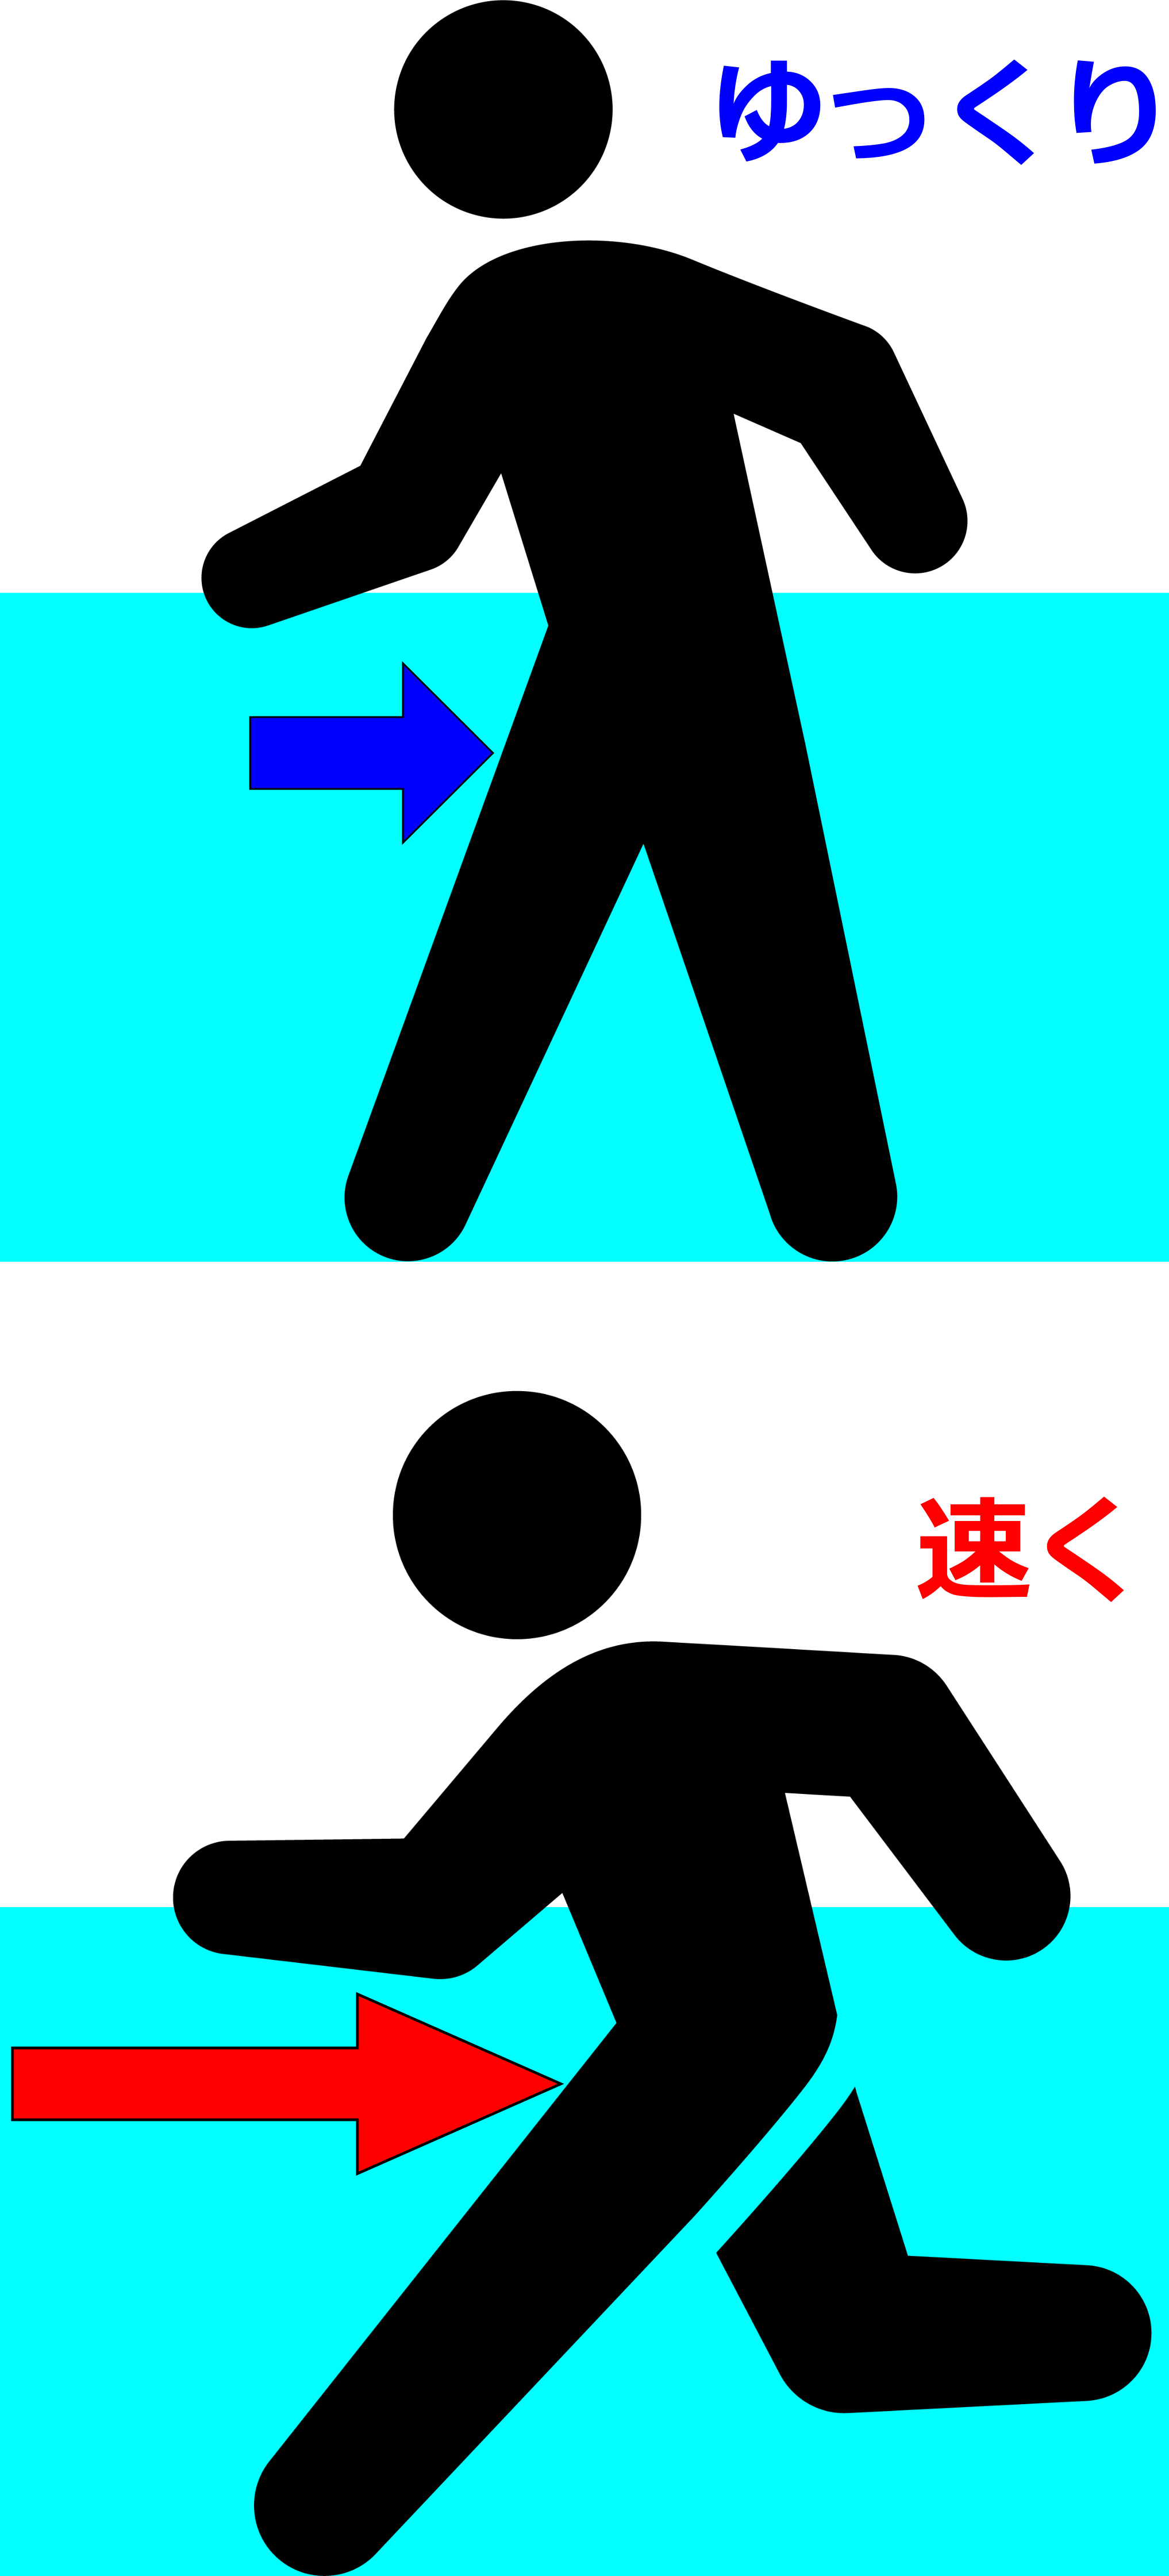
\includegraphics[width=.5\textwidth]{pool_walking.png}
			\end{center}
		\end{minipage}
		\caption{プールでの水中歩行}
		\label{pool_walk}
	\end{center}
\end{figure}

このことから、液体の性質として、変形させる速度が変わると生じる力も変わって、速い変形に対しては応力も大きくなることがわかります。


% \subsubsection{液体のモデル}
% 液体の持つこのような性質を表すモデルとして、以下の図 \ref{ekitai_model} に示したような水面に板を浮かべたモデルが良く使われます
% \footnote{
% 	流体のモデル化を行うときには、簡便のためにここで示したせん断変形モードだけを想定しますが、個体の場合と同様に伸長変形を考えることも同然できます。ここでは、その議論は割愛します。
% }。
% そして、変形を与え続けるための板の移動速度を「外的な刺激」として用います。

% \begin{figure}[htb]
% 	\begin{center}
% 		\begin{minipage}{0.5\textwidth}
% 			\Large
% 			水面に板を浮かべたモデル
% 			\begin{itemize}
% 				\item 水深方向に n+1 層に分割
% 				\item 水面の板との境目を0
% 				\item 水底との境目を n 
% 				\item 0 では板の速度vで移動
% 				\item n では地面との相対速度は0
% 			\end{itemize}
% 		\end{minipage}
% 		\begin{minipage}{0.3\textwidth}
% 			\begin{center}
% 			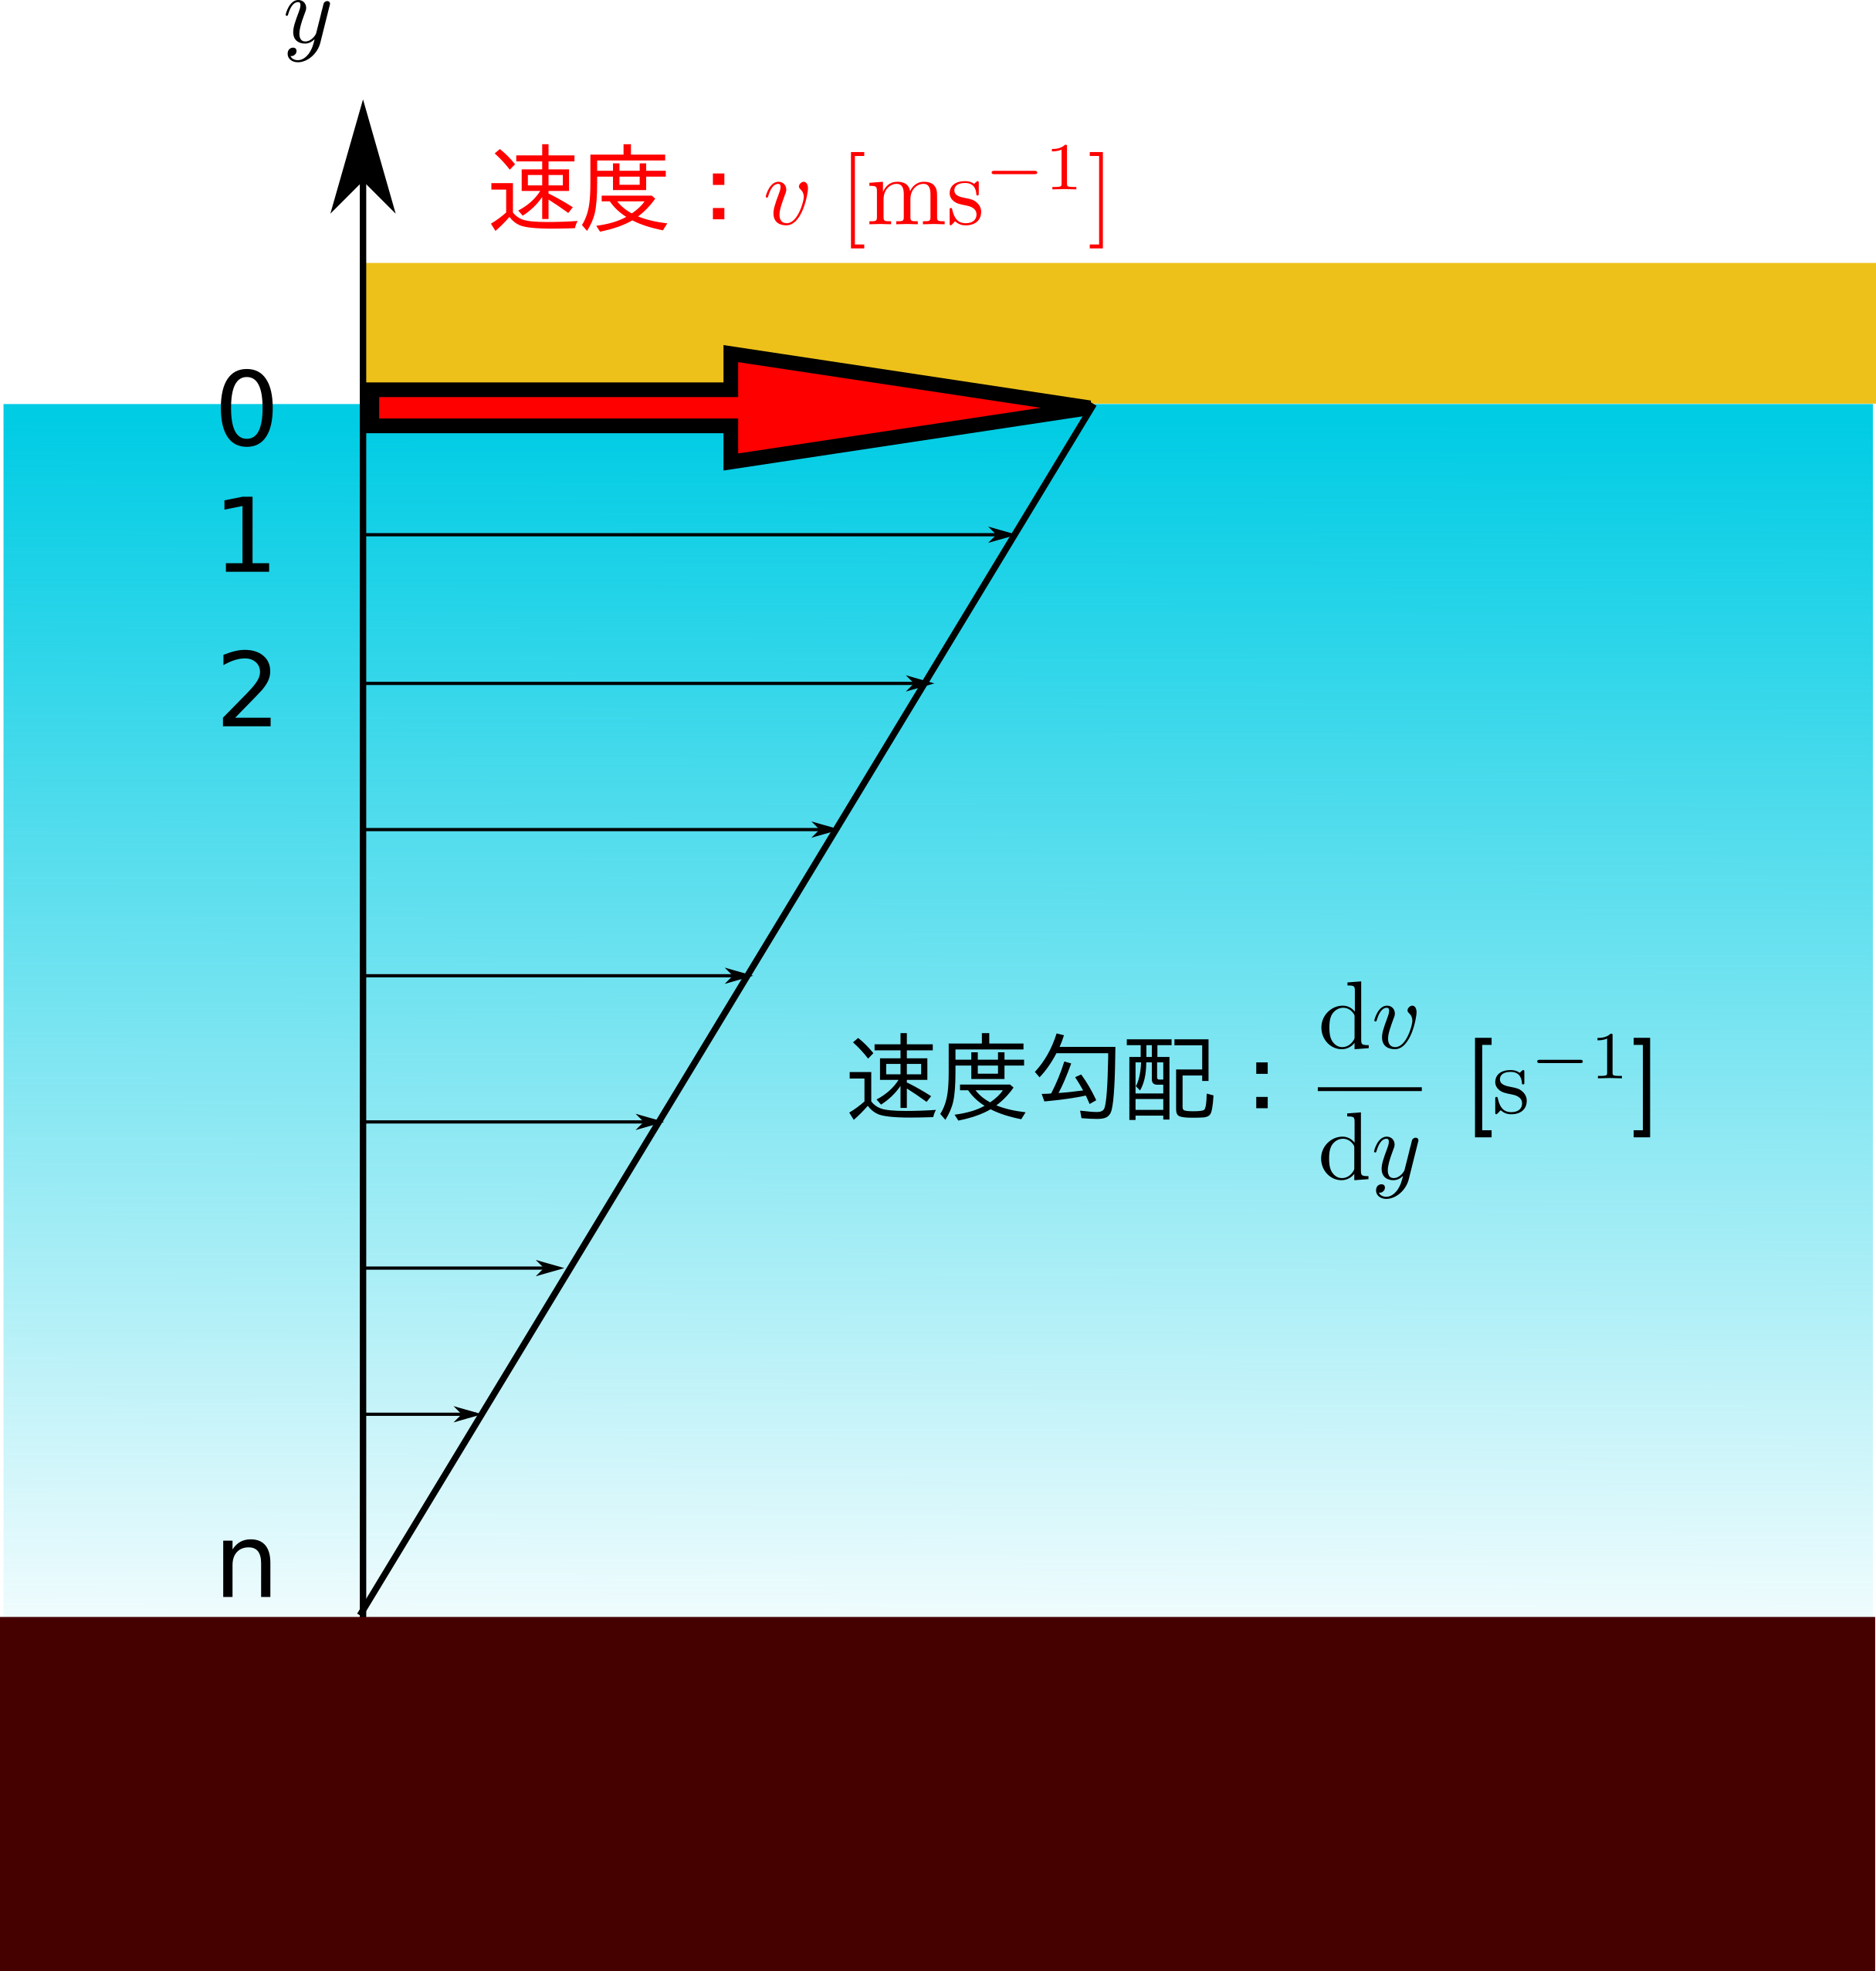
\includegraphics[width=.9\textwidth]{shear_3.png}
% 			\end{center}
% 		\end{minipage}
% 		\caption{液体の変形のモデル}
% 		\label{ekitai_model}
% 	\end{center}
% \end{figure}
% 液体を考えるときに重要な事項として、固体と接している液体はその相対的な移動速度が同じであるということがあります。
% したがって、図 \ref{ekitai_model} に示したように、移動する板と接している層は板と同じ速度 $v$ で流れますし、地面に接している層 $n$ は流れません。

% このとき、評価の対象である液体の内部では、水底と板との間の水深に応じて、流れる速度の分布が生じることが知られています。
% したがって、液体の流れる速度は、水深 $y$ の関数として $v(y)$ と表されることになり
% \footnote{
% 	この関数は、次章で説明する「微分」という考え方で整理され、$\dfrac{\mathrm{d} v}{\mathrm{d} y}$ という表式になります。
% }、速度勾配と呼ばれ、その単位は $[\mathrm{s^{-1}}]$ となります。
% このイメージ図では、速度勾配の傾きは一定となった最も単純な状態を表しています
% \footnote{
% 	この関係は、水深と速度勾配の間に線型関係が成立していることを表しています。
% 	なお、常に線型関係が成立するわけではなく、当然、非線形の関係もしばしば見受けられます。
% }
% 。

% ここで示した速度勾配は、せん断変形を記述する無次元量であるせん断ひずみ $\gamma$ の時間変化(微分)と捉えることも出来るため、以下の表式で表されることが多くなっています
% \footnote{
% 	ここで、せん断ひずみを表す $\gamma$ の上部に $\cdot$ をつけることで、ひずみの時間変化、すなわちせん断速度を表しています。
% }。
% \begin{align}
% 	\dfrac{\mathrm{d} v}{\mathrm{d} y} =\dot{\gamma} [s^{-1}]
% \end{align}

\subsection{液体の力学モデル}

\subsubsection{ ニュートンの法則}
では、液体の力学的な応答を記述するモデルはどうなるのでしょうか。
これは、古典力学の土台を築いた Sir Isaac Newton が、流れのせん断応力 $\tau$ とせん断速度 $\dot{\gamma}$ (速度勾配)との間に比例関係を見出しています。

実際の実験は、図 \ref{nijyu} に示したような二重になった円筒中に試料となる液体を入れ、内部の円筒を回転させながらそのときに生じる力を測定します。
内部に入った円筒の回転速度を変化させることでせん断速度を変化させ、そのときに生じるせん断応力との間に比例関係があることを見出しました。

この比例関係を式で表せば、
	\begin{align}
		\text{せん断応力} &= \text{比例定数} \times \text{せん断速度} \notag \\
		\tau &= \eta \dot{\gamma}
	\end{align}
式中で示した比例定数が、物質の流れ易さを表す指標である「粘度」となります。
\begin{figure}[htb]
	\begin{center}
		\begin{minipage}{0.6\textwidth}
			\large
			\begin{itembox}[l]{ニュートンの法則}
				\vspace{-3mm}
				\begin{align*}
					\text{せん断応力} &= \text{比例定数} \times \text{せん断速度} \notag \\
					\tau &= \eta \dot{\gamma}
				\end{align*}
				比例定数 $\eta$ が、物質の流れ易さを表す「粘度」
			\end{itembox}
		\end{minipage}
		\begin{minipage}{0.3\textwidth}
			\begin{center}
			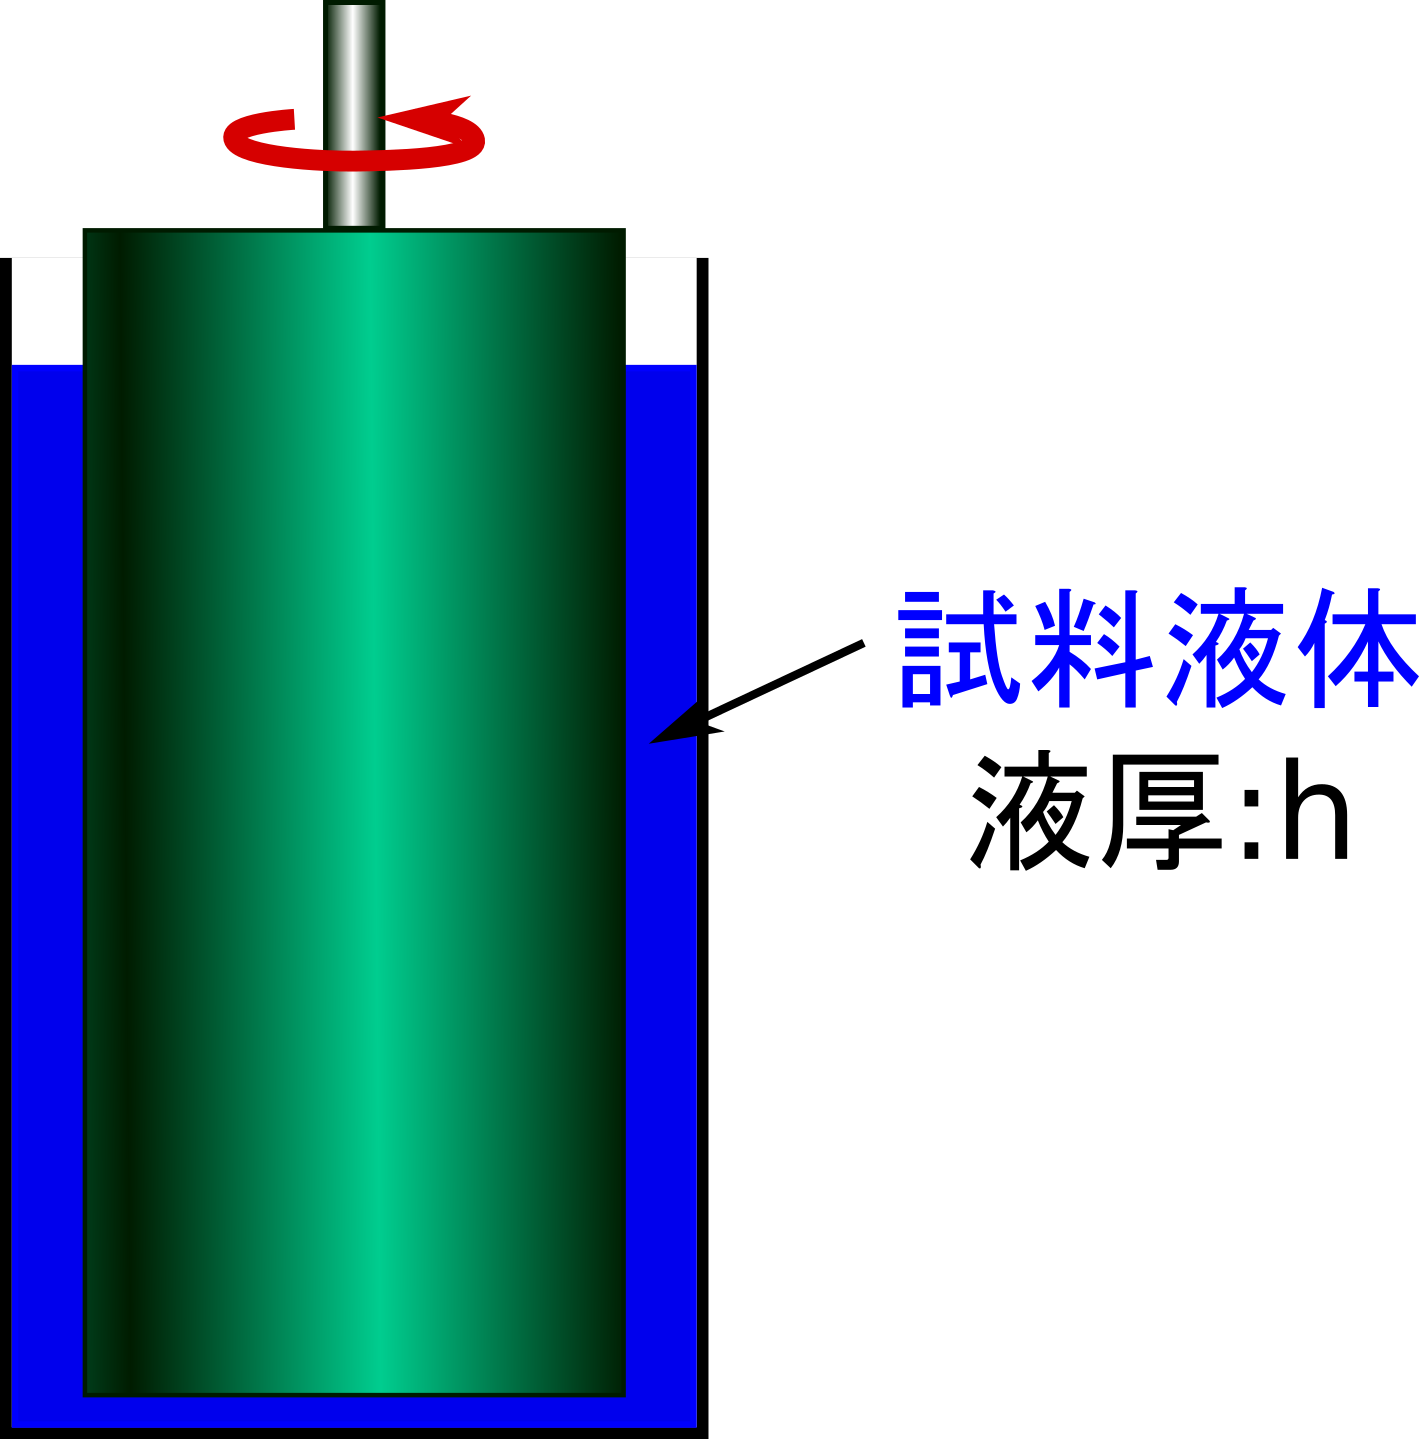
\includegraphics[width=.8\textwidth]{nijyu_entou.png}
			\end{center}
		\end{minipage}
		\caption{二重円筒による測定}
		\label{nijyu}
	\end{center}
\end{figure}

なお、粘度の単位は以下のようになります。
\begin{align}
	[\text{粘度}] &= \dfrac{[\text{せん断応力}]}{[\text{せん断速度}]} \notag \\
		&= \dfrac{[\mathrm{Pa}]}{[\mathrm{s^{-1}}]} = [\mathrm{Pa\cdot s}]
\end{align}


\subsubsection{液体の力学モデル}

ニュートンの法則が成り立つような液体の力学モデルをイメージ図とすると、図 \ref{flow_model} となります。
\begin{figure}[htbp]
	\begin{center}
		\begin{minipage}{0.55\textwidth}
			\large
			\begin{itembox}[l]{液体のモデル}
				\begin{itemize}
					\item 液体の振る舞いを表すモデル
					\item 右図のダッシュポット
					\item イメージとしては、水鉄砲
					\item 速くピストンを動かすと、\\抵抗が大。
				\end{itemize}
			\end{itembox}
			
		\end{minipage}
		\begin{minipage}{0.35\textwidth}
			\begin{center}
			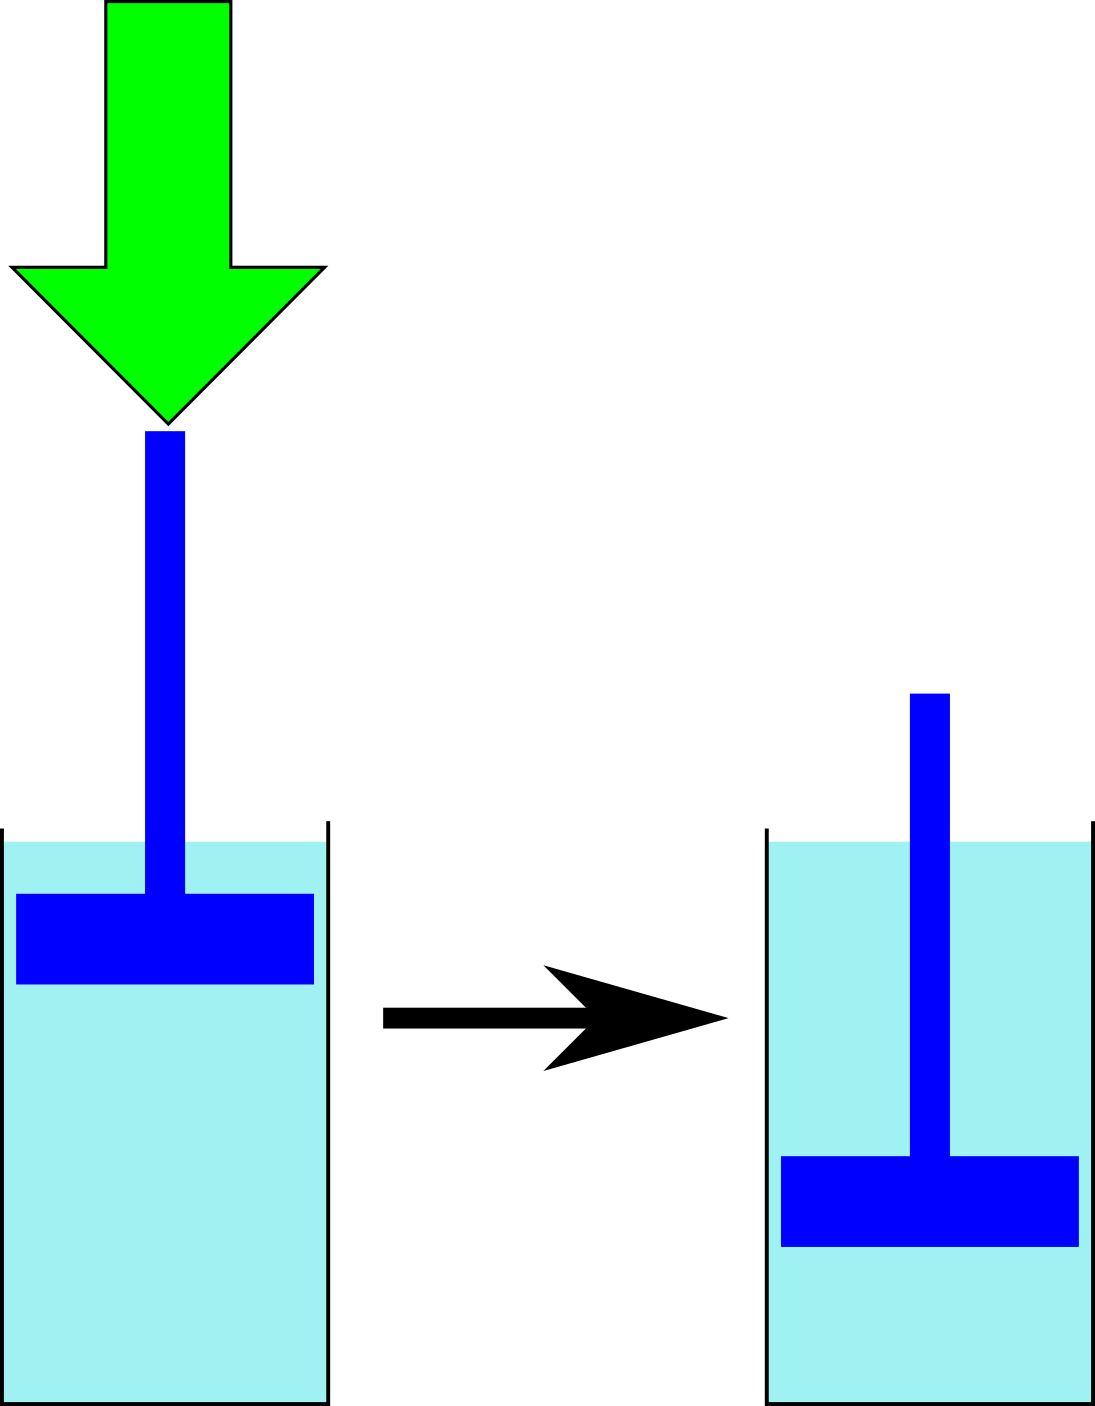
\includegraphics[width=.8\textwidth]{dashpot.png}
			\end{center}
		\end{minipage}
		\caption{液体の力学モデル}
		\label{flow_model}
	\end{center}
\end{figure}

このモデルは、液体の抵抗がその変形速度に比例するというニュートン流体の特性を表しています。

% ニュートンの法則に従った応答をする液体のことを、ニュートン流体と呼びます。
% 液体の内部では、「水深と速度勾配との間に線型関係が成立して、速度勾配の傾きが一定」になるような単純な流れ方をしていることになっています。

% このとき、深さ方向に見た場合にそれぞれの層の流れる速度は異なっていますので、層の間に生じているせん断応力もそれに比例して変化していることに注意してください。

\section*{この章のまとめ}

この章では、固体と液体という基本的な物質のふるまいを書き表す一番単純なモデルについて、説明を進めました。
	\begin{boxnote}
		\large
		\begin{itemize}
			\item 固体と液体という基本的な物質のありようについて、レオロジー的に考えていきます。
			\begin{itemize}
				\item 固体の最も基本的なモデルである弾性体という状態
				\item 刺激と応答を表すために、ひずみと応力を使うことで力学モデルが書けること
				\item 液体の応答について
				\item 液体の力学モデルが、「ひずみ速度\index{ひずみそくど@ひずみ速度}」で表されること
			\end{itemize} 
		\end{itemize}
	\end{boxnote}

	\newpage

	\begin{longartdeco}
		\begin{center}
		\emph{コラム:バリデーションの重要性}	
		\end{center}
	
		早逝されてしまった、元レオロジー学会長の上田さんという方がレオロジーの学び方のポイントとして、カエルの話をしていました。せっかくなので残して行きたいなと思い、ここに書いておくことにします。

	最初の話は、「茹でガエル」というもので、環境変化に関する寓話です。
	これは、1960年代の東西冷戦、1980年代の終末論、1990年代には温暖化に関連して取り上げられてきているようです。

	2つ目の話は、イソップ寓話に収録されている「二匹のカエル」というお話で、困難な状況でも頑張れば道は開ける(かも)というものです。
	上田さんは強引にクリームのダイラタンシーの話にしてレオロジーとつなげていました。
	結局、どっちのやり方がいいのかは、結果を見るまではわからないということなんで、自分のやり方を信じるしかないですね。

	「茹でガエル」

	カエルのような変温動物は、外部の温度環境によって自身の温度が変化します。
	したがって、本来は、気温が高くなって暑い場合は冷たい場所へ、また、気温が下がって凍えるときには暖かい場所へと移動する必要があります。
	カエルを熱い湯の中に入れてみると、居心地の良い場所へと慌てて逃げ出して行きます。
	でも、カエルを水の入ったビーカーに入れてゆっくりと水の温度を上げていくと、カエルは周りの温度が上がったことに気づかなくて、そのまま茹で上がって死んでしまいます。
	と書きましたが、これは似非科学的な作り話とのことです。

	人間も周りの環境が徐々に変化していっても気づかなくて、「アッと気づいたとき」には、逃げようのないとんでもない状況に追い込まれることがあります。
	ここから転じて、以下のような警句を表しています。
	「現状認識をしっかりと!」
	これは、周囲の変化に対して、常にきちんと対応しましょうということですね。

	「二匹のカエル」

	二匹のカエルが、ミルクのいっぱい入った壺の縁の周りを飛び跳ねていましたが、突然、二匹とも壺に落ちてしまいました。
	一匹のカエルは、「ああ、もう駄目だー!」と諦めてしまって、じっとして、結局溺れて死んでしまいました。
	もう一日のカエルは、「なんとかしよう」ともがいて、何度も何度も足を蹴って一生懸命泳ぎました。すると、足元のミルクがだんだんとチーズになって固まってきて、それを足がかりにして壺の外へと飛び出せました。
	これから得られる警句は、
	「現状分析するよりも行動を!」
	ということになります。
	まあ、変に周りが見えると、小賢しい考えにとらわれるので良くない場合もあるということです。
	
	\end{longartdeco}

    \newpage


    \question{演習問題 1}
    内容を振り返るために、以下に示した文章例の中から適切な記述のものを複数選んでください。
        \begin{qlist}
            \qitem 力と釣り合いについての、正しい言葉はどれでしょうか?
            \begin{qlist2}
                \qitem 静力学とは、相互作用する物体系の運動について議論します。
                \qitem 物質に力を加えたとき、物質の内部には外力の何倍もの大きな力が生じます。
                \qitem 力とは、物体の状態を変化させる原因となる作用で、その作用の大きさを表す物理量と考えられます。
                \qitem 力の釣り合いを議論するものが静力学です。
                \qitem 作用した力と釣り合う力が生じることを、「作用・反作用の原理」といいます。
            \end{qlist2}
        \vspace{3mm}
        \qitem 「力学的な刺激と応答」についての、正しい言葉はどれでしょうか?
            \begin{qlist2}
                \qitem 物質に刺激を与えるということは変形させるということに対応し、変形の結果として応力という応答が生じます。
                \qitem ひずみとは、変形の状態を表す尺度であり、初期状態からどれだけ変位したかを表す無次元量です。
                \qitem ひずみとは、変形度合いを表す長さの次元を持った物理量です。
                \qitem 物質に加えた外力と応力とは、力の大きさを表す全く同一の物理量です。
                \qitem 応力の表す意味は単位面積あたりに働く内部の力ということになります。
            \end{qlist2}
        \vspace{3mm}
        \qitem 弾性体のモデルについての、正しい言葉はどれでしょうか?
            \begin{qlist2}
                \qitem 弾性体であっても、いったん外力により変形すると、もう元には戻りません。
                \qitem 弾性体はあたかもバネのように取り扱うことができます。
                \qitem 弾性体を表すモデルはニュートンの法則であり、ダッシュポットでイメージできます。
                \qitem 弾性体のフックモデルでは全体のひずみに比例するのは応力です。
                \qitem フックモデルでの比例定数が弾性率であり、応力と同じ次元 [Pa] です。
            \end{qlist2}
        \vspace{3mm}
        \qitem 「液体の変形と応答」についての、正しい言葉はどれでしょうか?
        \begin{qlist2}
            \qitem 液体は、「外力によって変形されたら元には戻れない」流れるという性質を持った物質です。
            \qitem 液体に変形を与えると流れ、変形を止めれば応力も消えます。
            \qitem いったん変形を加えると、液体内部での応力はずっと維持されます。
            \qitem 液体は、変形させる速度が変わると生じる応力も変わります。
            \qitem 水中ではゆっくり歩いても水の抵抗は変化しません。
        \end{qlist2}
      \vspace{3mm}
        \qitem 液体のモデルについての、正しい言葉はどれでしょうか?
        \begin{qlist2}
            \qitem 液体の流れるという性質は、ニュートンの法則で整理できます。
            \qitem 液体はせん断速度に反比例して流れやすさが低下します。
            \qitem せん断応力は、せん断速度に比例します。
            \qitem その比例定数が、物質の流れやすさを表す指標である粘度となります。
            \qitem 液体の力学モデルは、ダッシュポットで表されます。
        \end{qlist2}
    \end{qlist}
    
    \question{演習問題 2}
    内容を振り返るために、テキストで用いた言葉を使って簡単な穴埋めを行ってください。
    
    \begin{qparts}
    \qpart 「弾性体の力学的な刺激と応答」について、以下の\qbox{(a)}から\qbox{(i)}までのカッコを埋めてください。
            \begin{qlist}
                \qitem 変形は、物質を一つの軸に沿って引き伸ばす「\qbox{}」とトランプのカードを横にずらしたような「\qbox{}」の二つに単純化できます。
                \qitem 伸張変形では、\qbox{}を\qbox{}で除したものがひずみとなります。
                \qitem 応力とは、物質の内部に生じている\qbox{}を表す物理量であり、その表す意味は単位面積あたりの\qbox{}ということになります。
                \qitem 応力と力の関係は以下のように書けます。
                \begin{align*}
                    \qbox{} = \dfrac{\qbox{}}{\qbox{}}
                \end{align*}
                % \qitem 一様な太さの棒を引っ張ったとき、棒の長手方向にはどの位置で切断したとしても、\qbox{}が働いていることに注意してください。
    
          \begin{itembox}[l]{選択肢}
            \begin{center}
              \begin{tabular}{lllll}
                1. 変形量	&2. せん断変形	&3. 力の大きさ	&4. 面積	&5. 応力\\
                6. 初期長さ	&7. 力		&8. 伸張変形				&9. 内部の力
              \end{tabular}
            \end{center}
          \end{itembox}
    
        \end{qlist}
    
    \qpart 弾性体と液体の力学応答について、以下の\qbox{(j)}から\qbox{(p)}までのカッコを埋めてください。
            \begin{qlist}
                \qitem 弾性体を表すモデルはフックの法則であり、以下のように書けます。
                    \begin{center}
                        \begin{minipage}{0.45\textwidth}
                            \begin{itemize}
                                \item \qbox{} $\varepsilon$ と比例して、
                                \item \qbox{} $\sigma$ が生じ、
                                \item 比例定数が\qbox{} $E$
                            \end{itemize}
                            \begin{align*}
                                \sigma = E \varepsilon
                            \end{align*}
                        \end{minipage}
                        \begin{minipage}{0.35\textwidth}
                            \begin{center}
                            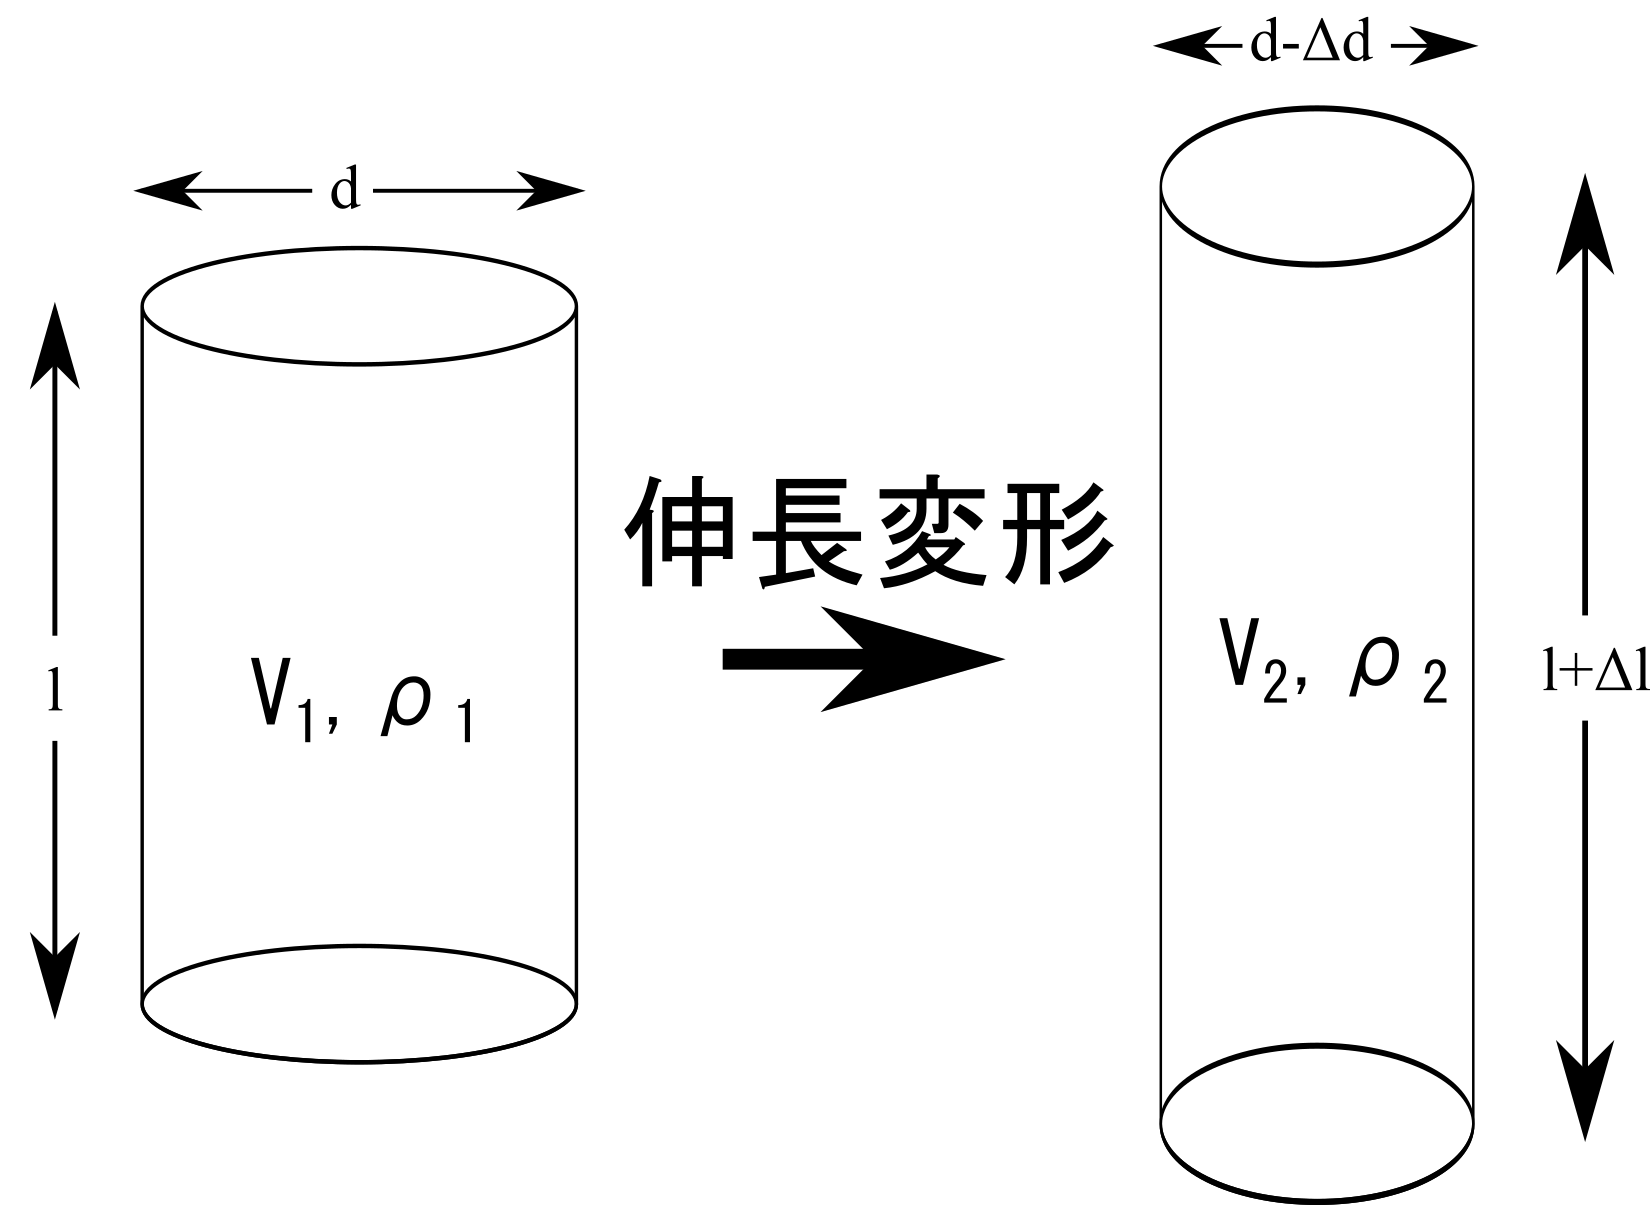
\includegraphics[width=.8\textwidth]{hook_law.png}
                            \end{center}
                        \end{minipage}
                    \end{center}
                \qitem 液体の評価は主としてそのひずみ速度を維持しやすい「\qbox{}」により行われる場合が多くなります。
                \qitem ニュートンの法則の比例関係を式で表せば以下のようになります。
                \begin{align*}
                    \text{\qbox{}} &= \text{\qbox{}} \times \text{\qbox{}} \notag \\
                    \tau &= \eta \dot{\gamma}
          \end{align*}
          
          \begin{itembox}[l]{選択肢}
            \begin{center}
              \begin{tabular}{llll}
                1. 伸張弾性率	&2. ひずみ速度	&3. 伸張ひずみ	&4. せん断応力\\
                5. 伸張応力 	&6. せん断変形	&7. 粘度		
              \end{tabular}
            \end{center}
          \end{itembox}
      \end{qlist}
    
    \end{qparts}
    
    \question{演習問題 3}
    数行程度の簡単な記述で構いませんので、以下の自由記述問題を考えてみてください。
    \begin{qlist}
    \qitem この章では、レオロジーのはじめの一歩として、その力学モデルについて簡単な説明を行ってきました。
    弾性体と液体の力学モデルの特徴についてそれぞれ簡単にまとめて、その大きな違いについて書いてみてください。
    \end{qlist}
    
\end{document}

\begin{thebibliography}{99}
	\bibitem{murakami}
	村上鎌吉 著, レオロジー基礎論
	\bibitem{masubuchi}
	増渕雄一 著, おもしろレオロジー
	\bibitem{osaki}
	尾崎邦弘 著, レオロジーの世界
	\bibitem{gakkai}
	日本レオロジー学会 編, 新講座・レオロジー
	\bibitem{yoshida}
	吉田武 著, オイラーの贈物
	\bibitem{nabata}
	名畑嘉之 著, 化粧品のレオロジー
\end{thebibliography}


\printindex

\end{document}